\documentclass[11pt, a4paper, french]{thloria}

% to be removed for final version
\ThesisDraft

\let\oldleftmark=\leftmark
\let\oldrightmark=\rightmark

\newcommand{\FaitMinitocs}{1} \newcommand{\CadresOvales}{1}
\newcommand{\FaitNomenclature}{1}

%%%%%%%%%%%%%%%%%%%%%%%%%%%%%%%%%%%%%%%%%%%%%%%%%%%%%%%%%
%%%% PACKAGES FONDAMENTAUX
%%%%%%%%%%%%%%%%%%%%%%%%%%%%%%%%%%%%%%%%%%%%%%%%%
\usepackage{ifthen}
\usepackage{ifpdf}


\usepackage[pdftex]{graphicx} % pour l'incusion de graphiques en pdf

\usepackage[intlimits]{amsmath} % amsmath, pour les maths
\usepackage{amssymb} % amssymb pour les symboles maths

%Pour pouvoir utiliser \allsectionsfont (utilis� dans le template)
\usepackage{sectsty}

% C'est quand m�me mieux, un pdf cliquable!
\usepackage[pdftex, colorlinks = true
   , pdfstartview = FitH 
   , linkcolor = blue
   , citecolor = blue
   , urlcolor = blue
   , bookmarksnumbered = true
   , bookmarksopen = true
   , pdfpagelabels
, pagebackref = true ]{tlhypref}


\usepackage{natbib} % citation of type (Dupont et al., 2013)
\renewcommand{\cite}{\citep}

\usepackage{morefloats} % accomodate large number of floats
\usepackage{placeins} 

\usepackage{fancybox} %pour encadrer les images en oval, shadow... Utilis� dans les macros

\usepackage{appendix} % pour annexes
\renewcommand\appendixname{Annexe}
\renewcommand\appendixpagename{Annexes}

%\usepackage{setspace} % pour singlespacing pour tabular



%%% Backref : permet de faire automatiquement des r�f�rences en arri�re cliquables dans la biblio, tr�s utile!
% setup the style of the backrefs from the bibliography %version ga�l compliqu�!
\RequirePackage[hyperpageref]{backref} % to be loaded after hyperref package
\newcommand{\backrefnotcitedstring}{\relax}%(Not cited.)
\newcommand{\backrefcitedsinglestring}[1]{(Page~#1.)}
\newcommand{\backrefcitedmultistring}[1]{(Pages~#1.)}
\renewcommand{\backreftwosep}{ et~} % seperate 2 pages
\renewcommand{\backreflastsep}{, et~} % seperate last of longer list
\renewcommand*{\backref}[1]{}  % Disable standard
\renewcommand*{\backrefalt}[4]{% Detailed backref
   \ifcase #1 %
   \backrefnotcitedstring%
   \or
   \backrefcitedsinglestring{#2}%
   \else
   \backrefcitedmultistring{#2}%
\fi}

% Si on veut des mini-tables des matieres :
\ifthenelse{\FaitMinitocs > 0}{
   \usepackage[french,nohints]{minitoc}%
   \mtcsetrules{minitoc}{off} % pour virer les lignes horizontales
   \mtcsettitle{minitoc}{} % pour virer le mot "<Sommaire"> au d�but des minitoc
   \setlength{\mtcindent}{0pt} % moins d'indentation � gauche des minitoc (d�faut 24pt)
   \mtcsetdepth{minitoc}{2} % pour voir sections et subsections.
}{}


%%%%%%%%%%%%%%%%%%%%%%%%%%%%%%%%%%%%%%%%%%%%%%%%%%%%%%%
% Pour pouvoir avoir des fleches depuis le texte vers des formules par exemple: TIKZ. Sert aussi pour l'index des notations, et pour les cadres
% http://www.fauskes.net/pgftikzexamples/global-nodes/
%%%%%%%%%%%%%%%%%%%%%%%%%%%%%%%%%%%%%%%%%%%%%%%%%%%%%%%
\usepackage{tikz,tkz-fct,tkz-2d}			% pour des supers graphiques trop cool, mieux que PSTricks.
\usetikzlibrary{snakes,arrows,shapes,backgrounds}
% For every picture that defines or uses external nodes, you'll have to apply the 'remember picture' style. To avoid some typing, we'll apply the style to all pictures.
\tikzstyle{every picture}+=[remember picture] 

% espace intelligent pour la fin d'une newcommand en tex (utilis� partout dans le fichier macro pour les maths)
\usepackage{xspace}

%gestion des unit�s !
\usepackage{sistyle}
%\SIstyle{German}   % Utile pour avoir une virgule avant les d�cimales et pas un point

% Les polices latex
\usepackage[latin1]{inputenc}
\usepackage[T1]{fontenc}
\usepackage{lmodern}
\usepackage[frenchb]{babel}

\usepackage[osf]{mathpazo}   % Palatino with smallcaps and oldstyle numbers
\usepackage[scaled]{helvet}  % Helvetica, scaled 95%


%Pour faire l'index des notations
\ifthenelse{\FaitNomenclature > 0}{
    \usepackage[norefpage,french,intoc]{nomencl}  %intoc rajoute une ligne dans la toc
    \renewcommand{\nomname}{\fontfamily{ppl}\selectfont Principales abbr�viations utilis�es} %Titre de la page
    \renewcommand{\pagedeclaration}[1]{~\dotfill\hyperpage{#1}}  %pour avoir des lignes de ... entre la description et le #page
    \renewcommand{\nomgroup}[1]{\bigskip}
    %\renewcommand{\nomgroup}[1]{%
    %\ifthenelse{\equal{#1}{A}}{\item[\textbf{\ChIntro}]}	  {
        %\ifthenelse{\equal{#1}{B}}{\medskip\item[\textbf{\ChMaxent}]}{
            %\ifthenelse{\equal{#1}{C}}{\medskip\item[\textbf{\ChImogene}]}{
                %\ifthenelse{\equal{#1}{D}}{\medskip\item[\textbf{\ChTrichomes}]}{
                    %\ifthenelse{\equal{#1}{E}}{\medskip\item[\textbf{\ChMuscle}]}{
                        %}}}}}
                    %}
                    %\def\ChCourantTitre{\ifcase\value{chapter} \or A\or B\or C \or D \or E\fi}
   %%%%%%%%%%%%%%%%%%%%%%%%%%%% D�finition de \ChCourantTitre ici!!!	


            \makenomenclature
         }{\newcommand{\nome}[2]{}}



% Pour ajouter des lignes comme biblio � la table des mati�res. Utilis� dans le template
         \usepackage[none]{tocbibind} 

%%%%%%%%%%%%%%%%%%%%%%%%%%%%%%%%%%%%%%%%%%%%%%%%%%%%%%%%%�
%%%% PACKAGES NON FONDAMENTAUX
%%%%%%%%%%%%%%%%%%%%%%%%%%%%%%%%%%%%%%%%%%%%%%%%%

%permet d'inclure des fichiers pdf directement dans le tex (articles en annexe), avec \includepdf[pages=-]{votre_fichier} 
         \usepackage{pdfpages}


         \usepackage{picins} %pour \parpic : images dans le texte � gauche ou � droite...

%http://www.cs.brown.edu/system/software/latex/doc/eqnarray.pdf
%Le fichier est � la racine du projet.
         \usepackage{equationarray}

% pour avoir les symboles \diameter, \frownie et \smiley
         \usepackage{wasysym}

% pour avoir les \ding{} : num�ros encercl�s
         \usepackage{pifont}

% pour des repr�sentation de vecteur sympa pour les physiciens
         \usepackage{vector}

% figures avec sous-figures et sous-captions:
         \usepackage[labelformat=empty, caption=true]{subfig}


\newcommand{\IncludePartOne}{1} 	\newcommand{\IncludePartTwo}{1}
\newcommand{\IncludePartThree}{1} \newcommand{\IncludePartFour}{1}

\newcommand{\IncludeAnnexes}{0} \newcommand{\IncludeAbstract}{1}

%\renewcommand{\baselinestretch}{1.5}




%%%%%%%%%%%%%%%%%%%%%%%%%%%%%%%%%%%%%%%%%%%%%%%%%%%%%%%%%%%%%%%%%%%%%%%%%%%%%%%%%%%%%%%%%%%%%%%%%%%%%%%%%%%%%%%%%%%%%%%%%%%%%%
%%%%%TOUT CE QUI CONCERNE TLORIA%%%%%%%%%%%%%%%%%%%%%%%%%%%%%%%%%%%%%%%%%%%%%%%%%%%%%%%%%%%%%%%%%%%%%
%%%%%%%%%%%%%%%%%%%%%%%%%%%%%%%%%%%%%%%%%%%%%%%%%%%%%%%%%%%%%%%%%%%%%%%%%%%%%%%%%%%%%%%%%%%%%%%%%%%%%%%%%%%%%%%%%%%%%%%%%%%%%%
%(cf _doc/TL-user.pdf pour plus de d�tails)
%-------------------------------------------------------------------
%                             En-tetes
%-------------------------------------------------------------------

% Les en-tetes: quelques exemples
%\UppercaseHeadings 
%\UnderlineHeadings
%\newcommand\bfheadings[1]{{\bf #1}}
%\FormatHeadingsWith{\bfheadings}
%\FormatHeadingsWith{\uppercase}
%\FormatHeadingsWith{\underline}
\newcommand\upun[1]{\uppercase{\underline{\underline{#1}}}}
\FormatHeadingsWith\upun

\newcommand\itheadings[1]{\textit{#1}}
\FormatHeadingsWith{\itheadings}

% pour avoir un trait sous l'en-tete:
\setlength{\HeadRuleWidth}{0.4pt}

%-------------------------------------------------------------------
%                         Les references
%-------------------------------------------------------------------

\NoChapterNumberInRef
\NoChapterPrefix

%-------------------------------------------------------------------
%                           Brouillons
%-------------------------------------------------------------------

% ceci ajoute une marque `brouillon' et la date
%\ThesisDraft



%%%%%%%%%%%%%%%%%%%%%%%%%%%%%%%%%%%%%%%%%%%%%%%%%%%%%%%%%%%%%%%%%%%%%%%%%%%%%%%%%%%%%%%%%%%%%%%%%%%%%%%%%%%%%%%%%%%%%%%%%%%%%%
%%%%%TOUT CE QUI NE CONCERNE PAS THLORIA%%%%%%%%%%%%%%%%%%%%%%%%%%%%%%%%%%%%%%%%%%%%%%%%%%%%%%%%%%%%%%%%%%%%%
%%%%%%%%%%%%%%%%%%%%%%%%%%%%%%%%%%%%%%%%%%%%%%%%%%%%%%%%%%%%%%%%%%%%%%%%%%%%%%%%%%%%%%%%%%%%%%%%%%%%%%%%%%%%%%%%%%%%%%%%%%%%%%

% Solution � la hache pour �viter les warning \oval et compagnie
\makeatletter
\renewcommand\@picture@warn{}
\makeatletter


% Un nouveau compteur pour les annexes
\newcounter{compteurannexes}
\renewcommand\thecompteurannexes{\Alph{compteurannexes}}


%%%% debut macro %%%% pour refaire les t�tes de chapitres
\makeatletter
\def\@makechapterhead#1{%
  %\vspace*{50\p@}% pour enlever l'espace avant le titre => minitoc rentre dans 1 page!
  \hrule
  \vspace*{10\p@}%
  {\parindent \z@ \raggedright \normalfont
    \ifnum \c@secnumdepth >\m@ne
      \if@mainmatter
        \huge{\fontfamily{ppl}\selectfont \bfseries \@chapapp\space \thechapter}
        \par\nobreak
          \vskip 10\p@
      \fi
    \fi
    \interlinepenalty\@M
    \Huge {\fontfamily{ppl}\selectfont #1}\par\nobreak
    \vspace*{10\p@}%
        \hrule
    \vskip 10\p@
}}
%%%%%Starred chapters (toc, lof, biblio)
\def\@schapter#1{\if@twocolumn
                   \@topnewpage[\@makeschapterhead{#1}]%
                 \else
                   \@makeschapterhead{#1}%
                   \@afterheading
                 \fi}
\def\@makeschapterhead#1{%
  \hrule
  \vspace*{10\p@}%
  {\parindent \z@ \raggedright \normalfont
    \interlinepenalty\@M
    \Huge{\fontfamily{ppl}\selectfont #1}
    \par\nobreak
    \vspace*{10\p@}%
        \hrule
    %\vskip 10\p@
  }}
\rmfamily
\makeatother
%%%% fin macro %%%%


% pour changer la police de toutes les sections
\allsectionsfont{\fontfamily{ppl}\selectfont}

% Num�rote les subsubsection pour pouvoir leur mettre un label et donc les voir appara�tre dans les minitocs
\setcounter{secnumdepth}{4}

% Mise en page des subsubsection avec un bullet, �crit en sffamily
\makeatletter
\renewcommand\subsubsection{\@startsection{subsubsection}{3}{10pt}%
                                     {-1.5ex \@plus -.2ex \@minus -.2ex}%
                                     {0.1ex \@plus.2ex}%
                                     {\sffamily\bf}}
\renewcommand\thesubsubsection{$\bullet$}          
\renewcommand*\l@subsubsection{\@dottedtocline{3}{7.0em}{1.5em}}                           
\makeatother              

% profondeur de la toc principale : 1 (minitoc : 2)
\setcounter{tocdepth}{1}


%%Pour avoir le titre du chapitre dans la liste des figures
%(xchapter est g�n�r� par minitoc)
\makeatletter
\let\l@xchapter\l@chapter
\makeatother

\begin{document}

%%%%%%%%%%%%%%%%%%%%%%%
%TITRE DES CHAPITRES
\newcommand{\ChIntro}{Introduction g�n�rale.}
\newcommand{\ChMaxent}{Mod�les de fixation des \TFs � l'ADN.}
\newcommand{\ChImogene}{{\em Imogene}: un algorithme d'identification de motifs et de modules de r�gulation transcriptionnelle}
\newcommand{\ChTrichomes}{�tude de la diff�renciation �pidermale chez la drosophile}
\newcommand{\ChMuscle}{�tude de la diff�renciation musculaire chez la souris}
\newcommand{\ChTest}{Chapitre d'exemples}


%%%%%%%%%%%%%%%%%%%%%%%%%%%%%%%%%%%%%%%%%%%%%%%%%%%%%%%%%%%%%%
%%%%%%%%% Le texte%%%%%%%%%%%%%%%%%%%%%%%%%%%
%%%%%%%%%%%%%%%%%%%%%%%%%%%%%%%%%%%%%%%%%%%%%%%%%%%%%%%%%%%%%%
\newcommand{\tf}{facteur de transcription\xspace}
\newcommand{\tfs}{facteurs de transcription\xspace}
\newcommand{\tfbs}{site de fixation de \tf\xspace}
\newcommand{\tfbss}{sites de fixation de \tf\xspace}
\newcommand{\tfbsss}{sites de fixation de \tfs\xspace}
\newcommand{\TF}{Facteur de Transcription\xspace}
\newcommand{\TFs}{Facteurs de Transcription\xspace}
\newcommand{\FT}{\TF}
\newcommand{\FTs}{\TFs}
\newcommand{\DI}{Information Directe\xspace}
\newcommand{\ID}{\DI}
\newcommand{\ft}{\tf}
\newcommand{\fts}{\tfs}
\newcommand{\TSS}{site de d�but de transcription}
\newcommand{\TSSs}{sites de d�but de transcription}
\newcommand{\CRM}{module de cis-r�gulation}
\newcommand{\crm}{\CRM}
\newcommand{\CRMs}{modules de cis-r�gulation}
\newcommand{\crms}{\CRMs}
\newcommand{\se}{\og shadow enhancers \fg}

\newcommand{\apriori}{\textit{a priori}\xspace}
\newcommand{\aposteriori}{\textit{a posteriori}\xspace}
\newcommand{\cad}{c'est-�-dire\xspace}
\newcommand{\etal}{\textit{et al.}\xspace}

\newcommand{\denovo}{\textit{de novo}\xspace}
\newcommand{\via}{\textit{via}\xspace}
\newcommand{\insitu}{\textit{in situ}\xspace}
\newcommand{\invitro}{\textit{in vitro}\xspace}
\newcommand{\invivo}{\textit{in vivo}\xspace}
\newcommand{\chip}{ChIP\xspace}
\newcommand{\chipchip}{ChIP-on-chip\xspace}
\newcommand{\chipseq}{ChIP-seq\xspace}
\newcommand{\dmel}{\textit{Drosophila melanogaster}\xspace}
\newcommand{\dromel}{\dmel\xspace}
\newcommand{\droso}{Drosophile\xspace}
\newcommand{\musmus}{\textit{Mus musculus}\xspace}
\newcommand{\celegans}{\textit{Caenorhabditis elegans}\xspace}
\newcommand{\ecoli}{\textit{Escherichia coli}\xspace}

\newcommand{\twi}{\textit{Twist}\xspace}
\newcommand{\myog}{\textit{Myog}\xspace}
\newcommand{\myod}{\textit{Myod1}\xspace}
\newcommand{\myf}{\textit{Myf5}\xspace}
\newcommand{\mrf}{\textit{Mrf4}\xspace}
\newcommand{\six}[1]{\textit{Six{#1}}\xspace}
\newcommand{\sixdko}[1]{\textit{Six1,4}\xspace}


%%%%%%%%%%%%%%%%%%%%%%%%%%%%%%%%%%%%%%%%%%%%%%%%%%%%%%%%%%%%%%
%%%%%%%%% Les maths%%%%%%%%%%%%%%%%%%%%%%%%%%%
%%%%%%%%%%%%%%%%%%%%%%%%%%%%%%%%%%%%%%%%%%%%%%%%%%%%%%%%%%%%%%

\newcommand{\Z}{\mathcal{Z}}

\newcommand{\pointformule}{\: .}
\newcommand{\virguleformule}{\: ,}
\newcommand{\finformule}{\vspace{-1cm}}

\newcommand{\OS}{\ensuremath{5^2 {\rm S}_{{1}/{2}}}\xspace}
\newcommand{\OPDD}{\ensuremath{5^2 {\rm P}_{{3}/{2}}}\xspace}
\newcommand{\OPDU}{\ensuremath{5^2 {\rm P}_{{1}/{2}}}\xspace}

\newcommand{\Etat}[1]{{| {#1} \rangle}}
\newcommand{\ket}[1]{\ensuremath{\left|#1\right\rangle}}
\newcommand{\bra}[1]{\left\langle #1\right|}


\newcommand{\Spin}[3]{\bra{#1} \widehat{S}_{#2} \ket{#3}}
\newcommand{\vr}{\ve{r}}
\newcommand{\rp}{\ve{r}^\prime}
\newcommand{\rpp}{\ve{r_\parallel}^{\prime\prime}}
\newcommand{\rA}{\ve{r_A}}
\newcommand{\uchap}{\widehat{u}}
\newcommand{\rrp}{(\ve{r},\rp)}
\newcommand{\rrpp}{(\ve{r},\rpp)}
\newcommand{\vu}{\ve{u}}

\newcommand{\FmF}[2]{{F=#1 , m_F=#2}\xspace}
\newcommand{\EtatFmF}[2]{\ensuremath{\Etat{ \FmF{#1}{#2} }}\xspace}
\newcommand{\EtatFprimemFprime}[2]{\ensuremath{\Etat{ F^\prime=#1 , m_F^\prime=#2 }}\xspace}
\newcommand{\EtatF}[1]{\ensuremath{\Etat{ F=#1 }}\xspace}
\newcommand{\EtatFprime}[1]{\ensuremath{\Etat{ F^\prime=#1 }}\xspace}
\newcommand{\mF}[1]{\ensuremath{\Etat{ m_F=#1 }}\xspace}
\newcommand{\mFprime}[1]{\ensuremath{\Etat{ m_{F^\prime}=#1 }}\xspace}
\newcommand{\mFv}[1]{\ensuremath{\Etat{ m_F }}\xspace}

\newcommand{\trdt}{\ensuremath{\EtatF{2} \to \EtatFprime{3}}\xspace}
\newcommand{\trud}{\ensuremath{\EtatF{1} \to \EtatFprime{2}}\xspace}


\newcommand{\keket}{\ensuremath{\left|\left|I=\frac32, m_I=\frac32; S=\frac12, m_s=\frac12 \right.\right\rangle}}
\newcommand{\kekett}{\ensuremath{\left|\left|I=\frac32, m_I=\frac32; S=\frac12, m_s=-\frac12 \right.\right\rangle}}
\newcommand{\kekettt}{\ensuremath{\left|\left|I=\frac32, m_I=\frac12; S=\frac12, m_s=\frac12 \right.\right\rangle}}
\newcommand{\kekk}{\EtatFmF{2}{2}}
\newcommand{\kek}{\EtatFmF{2}{1}}


\newcommand{\lambdaDB}{{\lambda_{\rm dB}}}

\newcommand{\mRb}{{m_{\rm Rb}}}
\newcommand{\Br}{{\ve{B\left( \ve{r} \right)}}}
\newcommand{\vectB}   {{\ve{B}}}
\newcommand{\vectBr}  {{\ve{B\left( \ve{r} \right)}}}
\newcommand{\vectBxyz}{{\ve{B\left( x,y,z \right)}}}
\newcommand{\modB}{{\Module{\vectB}}}
\newcommand{\modBr}{{\Module{\Br}}}

\newcommand{\omegaHF}{{\omega_{\rm hf}}}

\newcommand{\kb}{k_{\rm B}}
\newcommand{\muB}{\mu_{\rm B}}
\newcommand{\const}{{\mbox{const}}}

\newcommand{\Dix}[1]{\cdot 10^{#1}}

\newcommand{\Expo}[1]{\mathrm{e}^{\left(#1\right)}}

\newcommand{\ve}[1]{\overrightarrow{#1}}
\newcommand{\Module}[1]{\lvert #1 \rvert}

\newcommand{\Gradient}[1]{\ve{\nabla} \left( #1 \right) }
\newcommand{\Divergence}[1]{\ve{\nabla} \cdot #1 }

\newcommand{\rotr}{\ve{\nabla}_{\vr}}
\newcommand{\rotrp}{\ve{\nabla}_{\rp}}
\newcommand{\Erw}{\ve{E}(\vr,\om)}

\newcommand{\nonum}{\thispagestyle{empty}\addtocounter{page}{-1}}
\newcommand{\Ry}{Rydberg~}
\newcommand{\e}{\varepsilon}
\newcommand{\p}{\varphi}
\newcommand{\al}{\alpha}
\newcommand{\om}{\omega}
\newcommand{\de}{\delta}
\newcommand{\Om}{\Omega}
\newcommand{\ld}{\lambda}
\newcommand{\lV}{\lambda_V}
\newcommand{\lL}{\lambda_L}
\newcommand{\lac}{\lambda_{ac}}
\newcommand{\bsig}{{\boldsymbol\sigma}}
\newcommand{\si}{\sigma_i}
\newcommand{\sj}{\sigma_j}
\newcommand{\sh}{\sinh}
\newcommand{\ch}{\cosh}
\newcommand{\be}{\begin{equation}}
\newcommand{\ee}{\end{equation}}
\newcommand{\ds}{\displaystyle}
\newcommand{\bs}{\bigskip}


%\newcommand\numberthis{\addtocounter{equation}{1}\tag{\theequation}}
%\newcommand{\eq}[1]{\begin{equation}#1\end{equation*}}
%\newcommand{\eqn}[1]{\begin{equation}#1\end{equation}}
%\newcommand{\eqal}[1]{\begin{align*} #1 \end{align*}}
%\newcommand{\eqaln}[1]{\begin{align*} \numberthis#1 \end{align*}}
%\newcommand{\eqalacc}[1]{\[\left\{\begin{aligned}#1\end{aligned}\right.\]}
%\newcommand{\eqalaccn}[1]{\[\left\{\numberthis \begin{aligned}#1\end{aligned}\right.\]}

\newcommand{\Si}{\SI} % pr�vient les fautes de frappe!

\renewcommand{\tanh}{\mathrm{th}} % tangente hyperbolique
\renewcommand{\cosh}{\mathrm{ch}} % cosinus hyperbolique
\renewcommand{\sinh}{\mathrm{sh}} % sinus hyperbolique

\newcommand{\Bb}[3]{\ensuremath{\ve{B}_\text{biais}=(#1,#2,#3)}~G}

\newcommand{\omb}{\overline{\omega}}


\newcommand{\Vr}{\overrightarrow{r}}
\newcommand{\phir}{\phi(\Vr)}


\newcommand{\ReIm}[1]{\textup{#1}\,}
\renewcommand{\Re}{\ReIm{Re}}
\renewcommand{\Im}{\ReIm{Im}} 

\newcommand{\Gr}{\overleftrightarrow{G}}
\newcommand{\Gif}{\Gamma_{i\to f}}
\newcommand{\Gift}{\widetilde{\Gamma}_{i\to f}}
\newcommand{\Giftt}{\widetilde{\widetilde{\Gamma}}_{i\to f}}
\newcommand{\trif}{\ensuremath{\ket{i}\to\ket{f}}\xspace}

\newcommand{\pr}{^\prime}
\newcommand{\prpr}{^{\prime\prime}}



% Supprime de la version compil�e ce qu'il y a en argument : utile si on veut garder une trace de ce qui ne passe pas le barrage de la relecture!
\newcommand{\EnFaitNon}[1]{}

% Pour avoir des r�f�rences du style XX page YY
\newcommand{\FullRef}[1]{\ref{#1} page \pageref{#1}}
% Idem pour les �quations (rajoute des parenth�ses)
\newcommand{\FullEqRef}[1]{\eqref{#1} page \pageref{#1}}

% Pour rajouter un enlever localement une ligne � la page courante sans modifier tout le reste : tr�s utile pour la version finale
\newcommand{\AjouteLigne}{\enlargethispage{1\baselineskip}}
\newcommand{\RetireLigne}{\enlargethispage{-1\baselineskip}}

%%%%%%%%%%%%%%%%%%%%%%%%%%%%%%%%%%%%%%%%%%%%%%%%%%%%%%%
% TIKZ : Pour pouvoir avoir des supers jolies boites avec du texte et des formules exemple:
% http://www.fauskes.net/pgftikzexamples/boxes-with-text-and-math/
%%%%%%%%%%%%%%%%%%%%%%%%%%%%%%%%%%%%%%%%%%%%%%%%%%%%%%%
%%%%%%%%%%%%%%%%%%%%%%%%%%%%%%%%%%%%%%%%%%%%%%%%%%%%%%%
% Boite de D�finition
\tikzstyle{DefinitionBox}=[draw=black, fill=black!5, very thick, rectangle, rounded corners, inner sep=10pt, inner ysep=15pt]
\tikzstyle{DefinitionTitre}=[draw=black, rectangle, rounded corners, fill=white, text=black]
\newcommand{\Definition}[1]{%
\begin{center}\begin{tikzpicture}
\node [DefinitionBox] (box){%
	\begin{minipage}{0.92\textwidth}
		{\color{black}{#1}}
	\end{minipage}};
\node[DefinitionTitre, right=10pt] at (box.north west) {\sffamily D�finition\rmfamily};
\end{tikzpicture}\end{center}
}

%%%%%%%%%%%%%%%%%%%%%%%%%%%%%%%%%%%%%%%%%%%%%%%%%%%%%%%
% Boite de Notation
\tikzstyle{NotationBox}=[draw=black, fill=black!5, very thick, rectangle, rounded corners, inner sep=10pt, inner ysep=15pt]
\tikzstyle{NotationTitre}=[draw=black, rectangle, rounded corners, fill=white, text=black]
\newcommand{\Notation}[1]{%
\begin{center}\begin{tikzpicture}
\node [NotationBox] (box){%
	\begin{minipage}{0.92\textwidth}
		{\color{black}{#1}}
	\end{minipage}};
\node[NotationTitre, right=10pt] at (box.north west) {\sffamily Notation\rmfamily};
\end{tikzpicture}\end{center}
}

%%%%%%%%%%%%%%%%%%%%%%%%%%%%%%%%%%%%%%%%%%%%%%%%%%%%%%%
% Boite personnalisable
\tikzstyle{PersoBox}=[draw=black, fill=black!5, very thick, rectangle, rounded corners, inner sep=10pt, inner ysep=15pt]
\tikzstyle{PersoTitre}=[draw=black, rectangle, rounded corners, fill=white, text=black]
\newcommand{\Perso}[3]{%
\begin{figure}[!ht]
	\begin{center}\begin{tikzpicture}
	\node [PersoBox] (box){%
		\begin{minipage}{0.85\textwidth}
			{\color{black}{\small #3}}
		\end{minipage}};
	\refstepcounter{compteurencadres}\label{#2}
	\node[PersoTitre, right=10pt] at (box.north west) {\sffamily Encadr� \thecompteurencadres : #1\rmfamily};
	\end{tikzpicture}\end{center}
\end{figure}
}

%%%%%%%%%%%%%%%%%%%%%%%%%%%%%%%%%%%%%%%%%%%%%%%%%%%%%%%
% Boite de technique (un trait)
\tikzstyle{TechBox}=[draw=white, fill=black!1, rectangle, inner sep=5pt, inner ysep=10pt]
\tikzstyle{TechTitre}=[draw=black!1,  rectangle, fill=black!1, text=black]
\tikzstyle{TechLigne}=[color=black!30, line width=0.03cm, cap=round]
\newcommand{\Tech}[1]{%
\begin{center}\begin{tikzpicture}
\node [TechBox, below right,right=20pt] (box)
{%
    \begin{minipage}{0.85\textwidth}%
        {\color{black!85}{\footnotesize #1}}%
    \end{minipage}%
};
\node[TechTitre, right=0pt] at (box.north west) {\sffamily\small D�monstration\rmfamily};
\draw[TechLigne] (box.north west)--(box.south west);
\draw[TechLigne] (box.north west)++(0,-0.2)--++(1.9,0);
\end{tikzpicture}\end{center}}


%%%%%%%%%%%%%%%%%%%%%%%%%%%%%%%%%%%%%%%%%%%%%%%%%%%%%%%
% Boite d'Application num�rique
\tikzstyle{ApplicationNumeriqueBox}=[draw=green!80, fill=green!2, very thick, rectangle, rounded corners, inner sep=10pt, inner ysep=15pt]
\tikzstyle{ApplicationNumeriqueTitre}=[draw=green!80, rectangle, rounded corners, fill=white, text=black]
\newcommand{\AN}[1]{%
\begin{center}\begin{tikzpicture}
\node [ApplicationNumeriqueBox] (box){%
	\begin{minipage}{0.95\textwidth}
		{\color{black}{#1}}
	\end{minipage}};
\node[ApplicationNumeriqueTitre, right=10pt] at (box.north west) {\sffamily Application num�rique\rmfamily};
\end{tikzpicture}\end{center}
}

%%%%%%%%%%%%%%%%%%%%%%%%%%%%%%%%%%%%%%%%%%%%%%%%%%%%%%%
% Boite de Resultat important
\tikzstyle{ResultatBox}=[draw=red, fill=red!1, very thick, rectangle, rounded corners, inner sep=10pt, inner ysep=10pt]
\tikzstyle{ResultatTitre}=[draw=red, rectangle, rounded corners, fill=red, text=black]
\newcommand{\Resultat}[1]{%
\begin{center}\begin{tikzpicture}
\node [ResultatBox] (box){%
	\begin{minipage}{0.90\textwidth}
		{\color{black}{#1}\vskip-3mm}
	\end{minipage}};
%\node[ResultatTitre, right=10pt] at (box.north west) {R�sultat};
\end{tikzpicture}\end{center}
}

%%%%%%%%%%%%%%%%%%%%%%%%%%%%%%%%%%%%%%%%%%%%%%%%%%%%%%%
% Boite d'Interpr�tation
\tikzstyle{InterpretationBox}=[draw=blue, fill=blue!9, very thick,rectangle, rounded corners, inner sep=10pt, inner ysep=15pt]
\tikzstyle{InterpretationTitre}=[draw=blue, rectangle, rounded corners, fill=white, text=black]
\newcommand{\Interpretation}[1]{%
\begin{center}\begin{tikzpicture}\node [InterpretationBox] (box){%
	\begin{minipage}{0.95\textwidth}
		{\color{black}{#1}}
	\end{minipage}};
\node[InterpretationTitre, right=10pt] at (box.north west) {\sffamily Interpr�tation\rmfamily};
\end{tikzpicture}\end{center}}

%%%%%%%%%%%%%%%%%%%%%%%%%%%%%%%%%%%%%%%%%%%%%%%%%%%%%%%

%%%%%%%%%%%%%%%%%%%%%%%%%%%%%%%%%%%%%%%%%%%%%%%%%%%%%%%
% Boite de Remarque %%deux traits
\tikzstyle{RemarqueBox}=[fill=white, rectangle, inner sep=5pt, inner ysep=5pt]
\tikzstyle{RemarqueTitre}=[draw=white, thick, fill=white, text=black]
\tikzstyle{RemarqueLigne}=[color=black, line width=0.03cm, cap=round]
\newcommand{\Remarque}[1]{%
\begin{center}\begin{tikzpicture}
\node [RemarqueBox, below right] (box)
{%
    \begin{minipage}{0.85\textwidth}%
        {\color{black}{#1}}%
    \end{minipage}%
};
\node[RemarqueTitre, above right] at (box.north west) {\sffamily Remarque\rmfamily};
\draw[RemarqueLigne] (box.north west)++(0,0.6)--(box.south west);
\draw[RemarqueLigne] (box.north west)--++(2,0);
\draw (box.south west)++(-0.1,0)--(-0.1,0.6);
%\draw[very thick] (box.north east)--(box.south east);
\end{tikzpicture}\end{center}}

%%%%%%%%%%%%%%%%%%%%%%%%%%%%%%%%%%%%%%%%%%%%%%%%%%%%%%%
% Boite de Remarquee %%un trait, un titre, �crit petit
\tikzstyle{RemarqueeBox}=[fill=blue!2, rectangle, inner sep=5pt, inner ysep=5pt]
\tikzstyle{RemarqueeTitre}=[draw=white, thick, fill=white, text=black]
\tikzstyle{RemarqueeLigne}=[color=black, line width=0.03cm, cap=round]
\newcommand{\Remarquee}[2]{%
\begin{center}\begin{tikzpicture}
\node [RemarqueeBox, below right] (box)
{%
    \begin{minipage}{0.90\textwidth}%
        {\small \color{black}{#2}\normalsize}%
    \end{minipage}%
};
\node[RemarqueeTitre, above right] at (box.north west) {\sffamily Remarque~:~#1\rmfamily};
\draw[RemarqueeLigne] (box.north west)++(0,0.6)--(box.south west);
\draw[RemarqueeLigne] (box.north west)--++(2,0);
%\draw (box.south west)++(-0.1,0)--(-0.1,0.6);
%\draw[very thick] (box.north east)--(box.south east);
\end{tikzpicture}\end{center}}

%%%%%%%%%%%%%%%%%%%%%%%%%%%%%%%%%%%%%%%%%%%%%%%%%%%%%%%%%%%


%%%%%%%%%%%%%%%%%%%%%%%%%%%%%%%%%%%%%%%%%%%%%%%%%%%%%%%%%%%%%%
%%%%%%%%% Les figures%%%%%%%%%%%%%%%%%%%%%%%%%%%
%%%%%%%%%%%%%%%%%%%%%%%%%%%%%%%%%%%%%%%%%%%%%%%%%%%%%%%%%%%%%%
\newenvironment{fminipage}{%
\begin{Sbox}\begin{minipage}}
{%
\end{minipage}\end{Sbox}
\ifthenelse{\CadresOvales > 0}{\Ovalbox{\TheSbox}}{\TheSbox}
}

\newenvironment{cminipage}{%
\begin{Sbox}\begin{minipage}}
{%
\end{minipage}\end{Sbox}
\ifthenelse{\CadresOvales > 0}{\shadowbox{\TheSbox}}{\TheSbox}
}

\newcommand{\MinipageWidth}{15cm}
\newcommand{\CaptionWidth}{14.6cm}
\newcommand{\CaptionMargin}{0.4cm}
\newcommand{\FigWidth}{14.5cm}
\newcommand{\CaptionFig}[1]{\caption{\small{#1}}}
\newcommand{\CaptionTocCaptionFig}[2]{\caption[#1]{\small{#2}}}
\newcommand{\captionbf}[2]{\caption[#1]{\small \textbf{#1.}{#2}}}

% Les figures ombr�es *********************************************
\newenvironment{GaelFigureSh}[1][\MinipageWidth]{%
\begin{figure}[!ht]
\centering
\begin{cminipage}{#1}
\centering
\vspace{\CaptionMargin}
\pgfmathqparse{#1-\CaptionMargin-\CaptionMargin}
\begin{minipage}{\pgfmathresult pt}
\centering
}{%
\end{minipage}
\end{cminipage}
\end{figure}}
\newcommand{\bfigsh}{\begin{GaelFigureSh}}
\newcommand{\efigsh}{\end{GaelFigureSh}}

% Les figures normales *********************************************
\newenvironment{GaelFigure}[1][\MinipageWidth]{%
\begin{figure}[!ht]
\centering
\begin{fminipage}{#1}
\centering
\vspace{\CaptionMargin}
\pgfmathqparse{#1-\CaptionMargin-\CaptionMargin}
\begin{minipage}{\pgfmathresult pt}
\centering
}{%
\end{minipage}
\end{fminipage}
\end{figure}}
\newcommand{\bfig}{\begin{GaelFigure}}
\newcommand{\efig}{\end{GaelFigure}}

% Les figures : pleine page ***************************************
\newenvironment{GaelFigurep}[1][\MinipageWidth]{%
\begin{figure}[!htbp]
\centering
\begin{fminipage}{#1}
\centering
\vspace{\CaptionMargin}
\pgfmathqparse{#1-\CaptionMargin-\CaptionMargin}
\begin{minipage}{\pgfmathresult pt}
\centering
}{%
\end{minipage}
\end{fminipage}
\end{figure}}
\newcommand{\bfigp}{\begin{GaelFigurep}}
\newcommand{\efigp}{\end{GaelFigurep}}


%%%%%%%%%%%%%%%%%%%%%%%%%%%%%%%%%%%%%%%%%%%%%%%%%%%%%%%%%%%%%%
%%%%%%%%% Les tableaux%%%%%%%%%%%%%%%%%%%%%%%%%%%
%%%%%%%%%%%%%%%%%%%%%%%%%%%%%%%%%%%%%%%%%%%%%%%%%%%%%%%%%%%%%%
\newenvironment{CedTableau}[1][\MinipageWidth]{%
\begin{table}[!ht]
\centering
\begin{fminipage}{#1}
\centering
\vspace{\CaptionMargin}
\pgfmathqparse{#1-\CaptionMargin-\CaptionMargin}
\begin{minipage}{\pgfmathresult pt}
\centering
}{%
\end{minipage}
\end{fminipage}
\end{table}}
\newcommand{\btab}{\begin{CedTableau}}
\newcommand{\etab}{\end{CedTableau}}


%%%%%%%%%%%%%%%%%%%%%%%%%%%%%%%%%%%%%%%%%%%%%%%%%%%%
%% Pour faire des supers fleches d'highlight entre texte et �quation %%
%% http://www.fauskes.net/pgftikzexamples/global-nodes/
%% On d�finit un bout de fleche, et un d�part de fleche, puis on dit de faire les fleches....

\newcommand{\DepartHighlightColorNoTexte}[1]{ \tikz\node[fill=#1!20,draw, circle](From#1){};}

\newcommand{\DepartHighlightColor}[2]{ \tikz[baseline=(From#1.base)] {\node[fill=#1!20](From#1){#2};}}

\newcommand{\ArriveeHiglightColor}[2]{
\tikz[baseline=(To#1.base)] {\node[fill=#1!20](To#1){#2};}}

\newcommand{\MakeFlecheHighlightColor}[1]{ \begin{tikzpicture}
[overlay]\path[->](From#1)edge%[bend left]
(To#1);
\end{tikzpicture}}


%%%%%%%%%%%%%%%%%%%%%%%%%%%%%%%%%%%%%%%%%%%%%%%%%%%%%%%%%%%%%%
%%%%%%%%% Les listes%%%%%%%%%%%%%%%%%%%%%%%%%%%
%%%%%%%%%%%%%%%%%%%%%%%%%%%%%%%%%%%%%%%%%%%%%%%%%%%%%%%%%%%%%%
%check tick : \surd
%fl�che droite creuse : \triangleright
%rond : bullet 	
%%%REFERENCE : http://www.artofproblemsolving.com/LaTeX/AoPS_L_GuideSym.php


\newenvironment{maliste}[1]%
{ \begin{list}%
	{$\triangleright$}%
	{\setlength{\labelwidth}{10pt}%
	 \setlength{\leftmargin}{#1pt}%
	 %\setlength{\itemsep}{\parsep}
	\setlength{\itemsep}{0pt}
}}%
{ \end{list} }

\newenvironment{malistee}[1]%
{ \begin{list}%
	{$\to$}%
	{\setlength{\labelwidth}{0pt}%
	 \setlength{\leftmargin}{#1pt}%
	 %\setlength{\itemsep}{\parsep}
	\setlength{\itemsep}{0pt}
}}%
{ \end{list} }

\newenvironment{malistebullet}[1]%
{ \begin{list}%
	{$\bullet$\refstepcounter{subsubsection}}%
	{\setlength{\labelwidth}{0pt}%
	 \setlength{\leftmargin}{#1pt}%
	 %\setlength{\itemsep}{\parsep}
	%\setlength{\itemsep}{0pt}
}}%
{ \end{list} }

\newcommand{\blst}[1]{\begin{maliste}{#1}}
\newcommand{\elst}{\end{maliste}}
\newcommand{\blste}[1]{\begin{malistee}{#1}}
\newcommand{\elste}{\end{malistee}}
\newcommand{\blstbul}[1]{\begin{malistebullet}{#1}}
\newcommand{\elstbul}{\end{malistebullet}}

%%Liste personnalisable
\newenvironment{malisteperso}[2]%
{ \begin{list}%
	{$#2$}%
	{\setlength{\labelwidth}{10pt}%
	 \setlength{\leftmargin}{#1pt}%
	 %\setlength{\itemsep}{\parsep}
	\setlength{\itemsep}{0pt}
}}%
{ \end{list} }


%%%%%%%%%%%%%%%%%%%%%%%%%%%%%%%%%%%%%%%%%%%%%%%%%%%%%%%%%%%%%%
%%%%%%%%% Les annexes (c'est crad de mettre �a l� mais bon!) %
%%%%%%%%%%%%%%%%%%%%%%%%%%%%%%%%%%%%%%%%%%%%%%%%%%%%%%%%%%%%%%

\newcommand{\AnnexTitreCed}[4]
{
%\pagestyle{plain}
\renewcommand{\leftmark}{Annexe #1 - #2}
\renewcommand{\rightmark}{Annexe #1 - #2}
 %\hrule
  \vspace{15pt}%
  {\Huge \fontfamily{ppl}\selectfont \textbf{Annexe #1}}
   \par\nobreak
    \vspace{20pt}
   {\Huge \fontfamily{ppl}\selectfont #2}
    \vspace{10pt}
       \hrule
   \vskip20pt
	\refstepcounter{compteurannexes}\label{#3}
  \normalsize
  #4
  \EmptyNewPage
}


\newcommand{\Article}[1]
{
%\pagestyle{plain}
\renewcommand{\leftmark}{Article}
\renewcommand{\rightmark}{Article}
 \hrule
  \vspace{15pt}%
   {\Huge \fontfamily{ppl}\selectfont Article}
    \vspace{10pt}
       \hrule
   \vskip20pt
  \normalsize
  #1
  \EmptyNewPage
}



%%%%%%%%%%%%%%%%%%%%%%%%%%%%%%%%%%%%%%%%%%%%%%%%%%%%%%%%%%%%%%
%%%%%%%%% Pour la liste des notations %%%%%%%%%%%%%%%%%%%%%
%%%%%%%%%%%%%%%%%%%%%%%%%%%%%%%%%%%%%%%%%%%%%%%%%%%%%%%%%%%%%%


	% ************************************************************************
		% Pour fair une note dans la marge !
		% Command for inserting a todo item
		\definecolor{orange}{rgb}{1,0.5,0}
		\tikzstyle{notestyleright} = [right, draw=black, fill=blue!1]%, text width = 1cm]
		\tikzstyle{notestyleleft} = [notestyleright, left]
		\tikzstyle{connectstyle} = [draw = orange, thick]
		\newcommand{\todo}[1]{%
		% Add to todo list
		%\addcontentsline{tdo}{todo}{\protect{#1}}%
		%
		\begin{tikzpicture}[remember picture]%, baseline=7.5ex]%
		  \node [coordinate] (inText) {};
		\end{tikzpicture}%
		%
		% Make the margin par
		\marginpar[%
		{% Draw note in left margin
		 \tikz[remember picture] \path (0,0)++(1.8,0)++(-0.2,0)node[notestyleleft] (inNote) {\hyperlink{nomenclaturepage}{#1}};}%
		]{% Draw note in right margin
		  \tikz[remember picture] \path (0,0)++(0.2,0)node[notestyleright] (inNote) {\hyperlink{nomenclaturepage}{#1}};%
		}
		}

 %\ChCourantTitre est d�fini dans le fichier packages...
	\newcommand{\nome}[2]{%
      \nomenclature[\ChCourantTitre]{#1}{#2}%
      \todo{#1}%  ---------------------------------------la commande todo{truc} fout le truc dans la marge du bon cot�
  }


%%%%%%%%%%%%%%%%%%%%%%%%%%%%%%%%%%%%%%%%%%%%%%%%%%%%%%%%%%%%%%%%%%%%%%%%%%%%%%%%%%%%%%%%%%%%%%%%%%%%%%%%%%%%%%%%%%%%%%%%%%%%%%
%%%%%%%%%%%%%%%%%%%%%%%%%%%%%%%%%%%%%%%%%%%%%%%%%%%%%%%%%%%%%%%%%%%%%%%%%%%%%%%%%%%%%%%%%%%%%%%%%%%%%%%%%%%%%%%%%%%%%%%%%%%%%%
%%%%%%%%%%%%%%%%%%%%%%%%%%%%%%%%%%%%%%%%%%%%%%%%%%%%%%%%%%%%%%%%%%%%%%%%%%%%%%%%%%%%%%%%%%%%%%%%%%%%%%%%%%%%%%%%%%%%%%%%%%%%%%

      \OddHead={{\leftmark\rightmark}{\hfil\slshape\rightmark}}
      \EvenHead={{\leftmark}{{\slshape\leftmark}\hfil}}
      \OddFoot={\hfil\thepage}
      \EvenFoot={\thepage\hfil}
      \pagestyle{ThesisHeadingsII}
      
      %\ChapterPageStyle{ThesisHeadingsII}
      %\PartPageStyle{ThesisHeadingsII}

%-------------------------------------------------------------------
%                          Encadrements
%-------------------------------------------------------------------

% encadre les chapitres dans la table des matieres:
% (ces commandes doivent figurer apres \begin{document}
%\FrameChaptersInToc  
%\FramePartsInToc


%-------------------------------------------------------------------
%            Reinitialisation de la numerotation des chapitres
%-------------------------------------------------------------------
% Si la commande suivante est presente,
% elle doit figurer APRES \begin{document}
% et avant la premiere commande \part
%\ResetChaptersAtParts 

%-------------------------------------------------------------------
%               mini-tables des matieres par chapitre
%-------------------------------------------------------------------
% preparer les mini-tables des matieres par chapitre.
% (commande de minitoc.sty)
\ifthenelse{\FaitMinitocs > 0}{\dominitoc}{}


%-------------------------------------------------------------------
%                  ecriture de `Chapitre'
%                      dans la table des matieres
%-------------------------------------------------------------------
\WriteChapterLabelInToc

%%Changer les titres de toc et lof
\renewcommand{\contentsname}{Table des mati�res}
\renewcommand{\listfigurename}{Liste des figures}

%{\renewcommand{\baselinestretch}{1}
\thispagestyle{empty}

\begin{center}
{ \textbf{D{\'e}partement de Physique} \hfill \textbf{Laboratoire de Physique Statistique}\\
\textbf{\'Ecole Normale Sup{\'e}rieure} \hfill \null} %\vspace{0.5cm}
\end{center}
\vspace{-1cm}
%  Inclusion des chouettes de l'Ecole Normale
\begin{figure}[h,t]
\begin{center}

\includegraphics[width=0.3\textwidth]{figures/chouettes}
\end{center}
\end{figure}

%\vspace{2cm}

\centerline{\bfseries \sffamily \large TH\`ESE de DOCTORAT de
l'UNIVERSIT\'E PARIS 7} \vskip .5cm \centerline{\large
Sp{\'e}cialit{\'e}~: Physique Th�orique}\vskip 1.4cm

\centerline{\large pr{\'e}sent{\'e}e par}
\vskip .6cm

\centerline{\bfseries \sffamily \Large Marc SANTOLINI} \vskip .6cm

\centerline{\large pour obtenir le grade de DOCTEUR de
l'UNIVERSIT\'E PARIS 7}
 \vskip 1.5cm

\centerline{\line(1,0){450}} \vskip 0.4cm \centerline{\bfseries
\sffamily \LARGE 
%R�seaux g�n�tiques: mod�les d'interaction 
Analyse computationnelle des �l�ments cis-r�gulateurs
} \vskip
.2cm

\centerline{\bfseries \sffamily \LARGE  
   dans les g�nomes d'eucaryotes sup�rieurs
   %et applications biologiques
}

\centerline{\line(1,0){450}} \vskip 1.8cm

\centerline{\bfseries  \large Soutenue le ZZ septembre 2013}

\centerline{\large devant le jury compos{\'e} de~:} \vskip 1cm

\begin{center}
\begin{minipage}{14cm}
\large\centering
\begin{tabular}{lp{6.8cm}l}


\bf M.&\ \bf Vincent HAKIM\ \rm\dotfill&Directeur de th{\`e}se\vspace{.1cm}\\
\bf M.&\ \bf Martin Weigt \ \rm\dotfill&Rapporteur\vspace{.1cm}\\
\bf M.&\ \bf Emmanuel Barillot \ \rm\dotfill&Examinateur\vspace{.1cm}\\
\bf M.&\ \bf Alain Zider \ \rm\dotfill&Pr�sident du jury\vspace{.1cm}\\
\bf M.&\ \bf Massimo Vergassola \ \rm\dotfill&Rapporteur\vspace{.1cm}\\
& & \\
\bf M.&\ \bf Pascal Maire \ \rm\dotfill&Membre invit�\vspace{.1cm}\\

\end{tabular}
\end{minipage}
\end{center}

%}

\linespread{1.5}
%-------------------------------------------------------------------
%                          remerciements
%-------------------------------------------------------------------
\EmptyNewPage
\DontFrameThisInToc
 \hrule
  \vspace{15pt}%
  {\Huge \fontfamily{ppl}\selectfont \textbf{Remerciements}}
   \par\nobreak
    \vspace{15pt}
       \hrule
   \vskip20pt
	\normalsize
	

    Je tiens d'abord � remercier mon directeur de th�se, Vincent Hakim, qui m'a
    procur� un encadrement d'une tr�s grande qualit� au cours de ces quatre
    ann�es pass�es au Laboratoire de Physique Statistique de l'�cole Normale
    Sup�rieure. Sa disponibilit�, son discernement, sa curiosit�, son esprit
    critique, l'�tendue de sa culture scientifique dans les disciplines aux
    modes de r�flexion et aux langages si diff�rents que sont la physique
    fondamentale et la biologie, sa capacit� � extraire d'un probl�me l'essence
    qui satisfait l'intuition et � chasser le superflu, sa d�marche toujours
    rigoureuse vers le plus testable, le plus v�rifiable, le plus dicible, m�l�
    � une grande humilit� intellectuelle en font un chercheur exemplaire qui
    nourrit l'admiration, et je suis fier d'avoir pu apprendre � ses c�t�s.

    Je tiens par ailleurs � remercier Pascal Maire qui m'a accueilli
    � l'Institut Cochin et m'a permi de r�aliser une partie des exp�riences sur
    la diff�renciation musculaire expos�es dans cette th�se. Pascal a r�ussi
    � m'introduire avec beaucoup de p�dagogie � la g�n�tique et au
    d�veloppement, sujets qui m'�taient initialement tr�s �trangers. Son calme,
    sa patience, la clart� de ses raisonnements et son ouverture d'esprit ont
    grandement facilit� cette exp�rience interdisciplinaire et je lui en suis
    gr�.

    J'ai eu la chance de r�aliser plusieurs collaborations au cours de cette
    th�se, et par l� de go�ter � la satisfaction des travaux en groupe,
    l'apanage de l'interdisciplinarit�. D'abord, je remercie beaucoup Herv�
    Rouault, qui finissait sa th�se lors de mon arriv�e, et qui m'a �norm�ment
    apport� sur les plans informatique (c'est peu dire), scientifique et
    humain. Ses connaissances encyclop�diques en programmation me furent
    essentielles, et je le remercie de sa disponibilit� pour m'y avoir
    introduit. La collaboration avec Thierry Mora au LPS m'a permis de
    me plonger dans la physique des verres de spins et de garder un pied dans la
    physique pure et le langage qui lui est associ�, dans une th�se autrement
    tr�s port�e sur la biologie. Je remercie Thierry pour sa rigueur et sa
    clart�, ainsi que pour sa capacit� � savoir prendre du recul sur l'objet
    scientifique et le mettre en perspective. Sa connaissance d'un large corpus
    de philosophie des sciences en a fait un locuteur passionant.  Je remercie
    par ailleurs Serge Plaza et Fran�ois Payre du Centre de Biologie du
    D�veloppement de l'Universit� Paul Sabatier pour les nombreuses et
    fructueuses interactions que nous avons eues. J'ai beaucoup b�n�fici� de
    leur dynamisme et les remercie de leur accueil tr�s chaleureux lors de mes
    venues � Toulouse. Je remercie aussi Delphine Menoret qui finit sa th�se
    avec Serge et avec qui ce fut un plaisir de collaborer. Enfin, je remercie
    grandement Iori Sakakibara, post-doctorant � l'Institut Cochin, qui m'a
    accompagn� dans ma d�couverte des m�andres et de la complexit� de la
    biologie exp�rimentale.  Ses capacit�s de travail n'ont d'�gal que
    l'�tendue de la confiance qu'on peut lui accorder.

    J'ai pu b�n�ficier au cours de cette th�se d'un cadre particuli�rement
    agr�able, que ce soit au LPS comme � l'Institut Cochin. Je remercie le
    directeur du LPS Eric Perez pour sa proximit� et sa disponibilit�, les
    secr�taires Marie Gefflot, Annie Ribaudeau, Alinh Rin-Tybenszky et Nora
    Sadaoui ainsi que les ing�nieurs syst�me Zaire Dissi, R�my Portier et
    Fr�d�ric Ayrault pour leur efficacit�. Je suis aussi redevable � Maryse
    Derand, secr�taire de l'Institut Cochin, pour sa gentillesse et sa
    rapidit�.

    Ces ann�es ont �t� financ�es en partie par un contrat doctoral avec
    l'universit� Paris Diderot, et par l'Association Fran�aise contre les
    Myopathies (AFM), et je les remercie de leur confiance. Je remercie aussi
    l'Association DEPHY et notamment son pr�sident �douard Br�zin pour leur
    aide plus que bienvenue lors de la jonction cahoteuse des deux contrats.

    Cette longue p�riode de travail fut l'occasion de nouer des amiti�s
    pr�cieuses. Je remercie pour cela mes acolytes de la DC21, et en
    particulier Martin Retaux, Guilhem Sommeria-Klein et L�o Blondel avec qui
    j'ai pass� des moments formidables. Leur diversit� de culture et de points
    de vue m�l� � leur ouverture d'esprit en ont fait des compagnons id�aux, et
    nos discussions prolixes vont profond�ment me manquer. J'ai aussi pu
    b�n�ficier d'un entourage agr�able � l'Institut Cochin, et je remercie
    entre autres Alice, Laura, Morgane, Fabien, Philippe, Christophe, Julien,
    Romain, Josiane et Maud.

    Je remercie enfin mes parents pour les valeurs pr�cieuses qu'ils m'ont
    inculqu�es, pour m'avoir laiss� la plus grande libert� dans les choix qui
    furent les miens et m'avoir toujours soutenu quelque furent mes d�cisions.
    Je remercie aussi ma compagne Aya pour sa pr�sence et son soutien tout au
    long de cette th�se.

    Il est �vident qu'il resterait une longue prose � �crire pour remercier
    tous ceux qui ne figurent pas ici, famille, amis, professeurs ou
    chercheurs, dont l'apport affectif ou intellectuel a tacitement particip�
    � la r�alisation de ce travail. Il sauront que je les en remercie et les
    garde � l'esprit.


 


\tableofcontents

\WriteThisInToc\listoffigures 


\ifthenelse{\FaitNomenclature > 0}{ 
    \cleardoublepage% or \clearpage
    \markboth{\nomname}{\nomname}
   \printnomenclature[1.5cm]
   \hypertarget{nomenclaturepage}{} 
}{}

\input{packaging/nomenclature}


% La commande \mainmatter (nouvelle commande LaTeX2e) permet de passer a la
% numerotation arabe (ce que fait \pagenumbering{arabic}) et de faire commencer
% la nouvelle page 1 sur une page impaire. On evitera donc d'utiliser
% directement \pagenumbering{arabic}.
\mainmatter

\newpage
\newcommand{\intro}{Avant-propos}
\WriteThisInToc\addstarredchapter{\intro}\chapter*{\intro}\markboth{\slshape
\intro\hfil}{\slshape \intro\hfil}
\vskip7mm

Cette th�se se d�compose en cinq chapitres. Le premier chapitre consiste en une
introduction g�n�rale � la r�gulation transcriptionnelle chez les organismes
eucaryotes multicellulaires �tudi�s dans cette th�se (Drosophile et
mammif�res). 
%Cette introduction longue aborde � la fois les ph�nom�nes biologiques associ�s
%et leur mod�lisation math�matique. 
Les deux chapitres suivants traitent de la mod�lisation math�matique de la
r�gulation transcriptionnelle. D'abord, le chapitre $2$ utilise des donn�es
\invivo extensives de fixation de \tfs sur l'ADN et compare la capacit� de
diff�rents mod�les � les d�crire correctement.  Puis le chapitre $3$ pr�sente
Imogene, un algorithme de pr�diction de motifs et de modules de r�gulation
� partir de s�quences d'ADN poss�dant une fonction de r�gulation similaire. Cet
algorithme est une extension au cas des mammif�res d'un algorithme d�velopp�
pr�c�demment par Herv� Rouault dans le cas des Drosophiles. Nous en pr�sentons
par ailleurs une utilisation nouvelle comme classifieur de s�quences d'ADN
conduisant diff�rents motifs d'expression. Le chapitre $4$ pr�sente une
application directe de cet algorithme au cas de la diff�renciation des
trichomes chez la Drosophile.  La validation des pr�dictions a n�cessit� de
nombreuses exp�riences dont les m�rites reviennent � Delphine Menoret de
l'�quipe de Serge Plaza � l'Universit� Paul Sabatier de Toulouse.  Enfin, le
chapitre $5$ pr�sente diverses pr�dictions et validations exp�rimentales
concernant la diff�renciation musculaire chez la souris. La partie
exp�rimentale a �t� en grande partie l'{\oe}uvre de Iori Sakakibara de l'�quipe
de Pascal Maire � l'Institut Cochin, et j'ai aussi pu r�aliser certaines des
exp�riences (qPCR, tests Lucif�rase, mutagen�ses\ldots) sous sa direction ainsi
que celle de Pascal Maire.

Les chapitres $2$, $3$, $4$ et $5$ sont organis�s autour d'articles en anglais
d�crivant le travail r�alis�. Afin de faciliter leur lecture, les concepts
sous-jacents et les travaux ant�rieurs sont introduits en d�but de chapitre.

Enfin, la version pdf de ce manuscrit contient de nombreux liens hypertexte
rendant la lecture plus ais�e. Dans la table des mati�res et la liste des
figures, les titres pointent vers l'item d�crit.  Dans le corps du texte, les
travaux cit�s pointent vers la r�f�rence correspondante dans la bibliographie,
et il est possible de revenir au texte en cliquant sur le num�ro de page
c�toyant la r�f�rence.



%\part{Premi�re partie}
%%%%%%%%%%%%%%%%%%%%%%%%%%%%%%%%%%%%%%%%%%%%%%%%%%%%%%%%%%%%%%%%%%%%%%%%%%%%%%%%%%%%%%%%%%
\chapter{\ChIntro}
\adjustmtc
\minitoc
\newpage
\vskip7mm
aller rapidement sur nouvelles techniques.
statistiques du genome


\section{La diff�renciation cellulaire}

\subsection{Qu'est-ce que le ph�notype d'une cellule?}

\subsection{Les cellules se sp�cialisent au cours du d�veloppement}

\bfig
\includegraphics[width=0.5\textwidth]{figures/furusawa-epigenetic-landscape.pdf}
\captionbf{Le paysage de la diff�renciation cellulaire}{
   Figure tir�e de \cite{Furusawa2012p3898}.
   \textbf{A.} Paysage �pig�n�tique tel qu'imagin� par Waddington
   \cite{waddington1957strategy} en r�sonance avec la notion de paysage
   �nerg�tique en physique. Le d�veloppement cellulaire est repr�sent�
   par une bille d�valant un paysage compos� de diff�rentes vall�es s�par�es
   par des barri�res montagneuses, repr�sentant les diff�rents types
   cellulaires et leur robustesse face aux fluctuations.  
   \textbf{B.} Repr�sentation dynamique de l'�volution des �tats cellulaires.
   Le ph�notype est ici caract�ris� par l'expression de
   trois prot�ines A, B et C, dont l'�volution dans le temps peut �tre
   repr�sent�e par une trajectoire dans un espace tridimensionnel.
   Les �tats souche et diff�renci�s sont caract�ris�s par des bassins
   d'attraction correspondant � diff�rents types cellulaires.
} 
\label{fig-furusawa-epigenetic-landscape}
\efig

\subsection{Les cellules sont reprogrammables}
Fibroblastes, IPS : seulement un ou quelques facteurs suffisent � changer le
ph�notype d'une cellule.


\bfig
\includegraphics[width=0.8\textwidth]{figures/siggia-fate.pdf}
\captionbf{Vision g�om�trique des transitions entre types cellulaire}{
   Figure tir�e de \cite{Corson2012p3973} sch�matisant le processus de
   diff�renciation des cellules de la vulve de \celegans.
   \textbf{A.} La cellule est dans un �tat pr�curseur repr�sent� par une
   bille au fond d'une vall�e.
   \textbf{B.} La cellule est dans �tat dit \textit{comp�tent} o� elle peut basculer
   vers diff�rents destins cellulaires.
   \textbf{C.} Un signal externe repr�sent� par une fl�che rouge modifie le
   paysage de mani�re � favoriser l'un des �tats finaux possibles.
} 
\efig


\bfig
\includegraphics[width=\textwidth]{figures/graf-cells-lineages.pdf}
\captionbf{Diff�rents exemples de reprogrammation cellulaire}{
   Figure tir�e de \cite{Graf2009p2592}. Exemples d'exp�riences de
   surexpression ou d'ablation de \fts qui aboutissent � des changements de
   destins cellulaires.
} 
\efig

$\rightarrow$ comment interpr�ter ces r�sultats?

\section{Les r�seaux de r�gulation g�n�tique}

\subsection{Vision cybern�tique de la cellule}
Monod, Jacob. Promoteurs. 
\subsection{Divers modes de r�gulation}
Enhancers, �pig�n�tique, post-transcriptionnelle, etc.

$\rightarrow$ quels outils pour exhiber cette circuiterie?


\bfig
\includegraphics[width=\textwidth]{figures/graf-differentiation-landscape.pdf}
\captionbf{Les antagonismes entre \tfs sculptent le paysage des destins
cellulaires}{
   Figure tir�e de \cite{Graf2009p2592}. Vision g�om�trique de la
   diff�renciation cellulaire inspir�e de Waddington (voir
   fig.\ref{fig-furusawa-epigenetic-landscape}).
} 
\efig

\section{D�crire les interactions au seins des r�seaux.}

\begin{malistebullet}{15}
\item R�gulation transcriptionnelle. Facteurs de transcription. Diffusion, fixation. \\
\item   Mod�les math�matiques (PWM, biophysiques). \\
\item   Coop�rativit�, fonctions logiques, coefficients de Hill (Uri Alon).\\
\item   Donn�es biologiques grande �chelle : \chipseq etc\ldots Bioinformatique.\\
\item   ENCODE, Taipale, etc.\\
\item   Evolution de la r�gulation Odom, Sinha.\\
\end{malistebullet}


\bfig
\includegraphics[width=.8\textwidth]{figures/wasserman-transcriptional-regulation.pdf}
\captionbf{Les diff�rentes composantes de la r�gulation transcriptionnelle}{
   Figure tir�e de \cite{Wasserman2004p624}. Les \TFs se fixent � des sites
   sp�cifiques de longueur $\sim10$bp qui peuvent �tre proximaux (promoteur,
   premiers introns) ou distaux (plus de $100$kb) d'un \TSS. Diff�rents \TFs
   peuvent s'assembler sur des r�gions d'ADN de taille typique $\sim 1000$bp
   appel�es \CRMs afin de conduire � une r�gulation sp�cifique, par simple effet
   de communaut� par exemple lorsque la fixation de tous les \tfs est requise pour
   que la r�gulation op�re. Les interactions entres les \tfs et diff�rents
   cofacteurs stabilisent la machinerie d'initiation de transcription pour
   permettre l'expression g�n�tique. La r�gulation distale est quant � elle
   fortement d�pendante de la structure tridimensionnelle de la chromatine.
   tridimensionnelle.
} 
\efig

\subsection{Le mod�le PWM}
Le mod�le PWM est le mod�le le
plus simple d�crivant l'�nergie de fixation entre un \tf et un site de
fixation sur l'ADN. Ce mod�le est bas� sur l'hypoth�se que l'�nergie
de fixation � un site est la somme des �nergies de fixation � chaque
nucl�otide. Si la concentration du \tf est faible, ce mod�le se r�duit � un
mod�le biophysique.

\bfig
\includegraphics[width=.7\textwidth]{figures/wasserman-PWM.pdf}
\captionbf{Construction et utilisation du mod�le PWM}{
   Figure tir�e de \cite{Wasserman2004p624}. (a) Supposons connus un certain nombre
   de sites de fixation d'un \tf (dans ce cas MEF2).(b) S�quence consensus
   correspondante utilisant les symboles IUPAC. (c) Une matrice de fr�quence
   est construite, indiquant pour chaque nucl�otide sa multiplicit� � une
   position donn�e dans le site. (d) La PWM est simplement construite en
   prenant le logarithme relatif des fr�quences PWMs par rapport aux fr�quences
   \textit{background} des nucl�otides. (e) Le score (ou �nergie) d'une s�quence d'ADN
   donn�e est calcul� en additionnant les poids PWMs correspondant. (f) La PWM
   peut �tre repr�sent�e sous forme de logo \cite{Giocomo2011p3442}. Dans cette
   repr�sentation, la hauteur d'une colonne repr�sente le contenu en
   information ou information relative moyenne d'une position, et la taille des
   bases refl�te leur fr�quence observ�e.
   
} 
\efig


\bfig
\includegraphics[width=.6\textwidth]{figures/hardison-enhancer-states.pdf}
\captionbf{Les �tats �pig�n�tiques des CRMs}{
   Figure tir�e de \cite{Hartwell1999p560}.
} 
\efig

\bfig
\includegraphics[width=\textwidth]{figures/hardison-CRM-prediction.pdf}
\captionbf{Approches pour la pr�diction des CRMs}{
   Figure tir�e de \cite{Hartwell1999p560}.
} 
\efig

\bfig
\includegraphics[width=\textwidth]{figures/hardison-CRM-test.pdf}
\captionbf{M�thodes de validation des CRMs}{
   Figure tir�e de \cite{Hartwell1999p560}.
} 
\efig


\bfig
\includegraphics[width=.4\textwidth]{figures/furey-chipseq.pdf}
\captionbf{�tapes d'une exp�rience de \chipseq}{
   Figure tir�e de \cite{Furey2012p3920}.
} 
\efig

\bfig
\includegraphics[width=.8\textwidth]{figures/furlong-eve-enhancers-to-stripes.pdf}
\captionbf{Diff�rents CRMs conduisent � diff�rents patterns d'expression}{
   Figure tir�e de \cite{Liu2009p556}.
} 
\efig

\bfig
\includegraphics[width=\textwidth]{figures/furlong-network-evolution.pdf}
\captionbf{}{
   Figure tir�e de \cite{Liu2009p556}.
} 
\efig


Visualisation sur UCSC.



\newpage 

%%%%%%%%%%%%%%%%%%%%%%%%%%%%%%%%%%%%%%%%%%%%%%%%%%%%%%%%%%%%%%%%%%%%%%%%%%%%%%%%%%%%%%%%%%
\chapter{\ChMaxent} 
\label{ch:maxent}
%\adjustmtc
\minitoc
\newpage
\section*{Introduction du chapitre \thechapter}

Dans cette partie, nous nous int�ressons � la description de l'interaction
entre les \fts et leurs sites de reconnaissance sur l'ADN.  Pendant longtemps,
la qualit� de cette description a �t� limit�e par la quantit� de donn�es
disponibles. Ainsi, les exp�riences de type SELEX (voir
\ref{sub:approches_invitro}), o� des exp�riences de \chip au cas par cas
permettaient de r�cup�rer de l'ordre de quelques dizaines de sites de fixation
pour un TF d'int�r�t. Or, le mod�le PWM, qui est le mod�le le plus simple (en
terme de nombre de param�tres) que l'on puisse b�tir pour d�crire l'interaction
poss�de d�j� plusieurs dizaines de param�tres -- les fr�quences des nucl�otides
� chaque position --. 

Ces donn�es ne permettaient donc pas d'explorer plus en avant des mod�les plus
complexes de fixation incluant par exemple des termes d'interaction entre
nucl�otides au sein des sites de fixation. Cependant, les avanc�es r�centes en
s�quen�age � haut d�bit ont permis l'obtention de donn�es tr�s grande �chelle,
que ce soit \invivo par \chipseq ou \invitro par HT-SELEX (voir
\ref{sec:mesures_exp}). Le nombre de sites de fixation obtenus est de l'ordre
de quelques milliers, ce qui permet de contraindre des mod�les de fixation plus
complexe que le mod�le PWM.

En utilisant des donn�es \chipseq pour un grand nombre de \fts de la Drosophile
et des vert�br�s, nous avons contraint diff�rents mod�les de fixation incluant
implicitement ou explicitement des interactions entre nucl�otides. Nous les
avons compar�s sur leur capacit� � d�crire les statistiques de fixation TF-ADN
observ�es \invivo. Nous pr�sentons pr�alablement un survol des observations et
mod�les existant au sujet des corr�lations dans les sites de fixations de \fts.

\section{Observations de corr�lations au sein des TFBS}
\label{sec:corr_lations_au_sein_des_sites_de_fixation_de_tfs}

Diff�rents travaux ont mis en exergue l'existence de corr�lations entre
nucl�otides au sein des sites de fixation de TFs. Parce que limit�es par la
quantit� de donn�es alors possible � obtenir, les premi�res �tudes de ce genre
ont centr� leur attention sur quelques corr�lations importantes pour des cas
particuliers. Ainsi, \citet{Man2001fk} ont observ� que la prot�ine Mnt induit
des corr�lations entre les positions $16$ et $17$ de ses sites de
reconnaissance \invitro. Ils ont mesur� exp�rimentalement la sp�cificit� aux
sites de liaisons contenant tous les variants possibles � ces deux positions.
Ils ont ainsi observ� que la mutation de la base consensus C en position 17
induisait un changement de pr�f�rence en position 16 de la base A vers la base
C. Par ailleurs, \citet{Bulyk2002uq} ont montr� que la prot�ine EGR$1$ induisait
des corr�lations au sein d'un triplet de nucl�otides central de leur site de
reconnaissance. La prise en compte de ces corr�lations dans l'�nergie de
fixation permettait alors d'am�liorer la description des donn�es par rapport au
mod�le additif PWM.

� une plus grande �chelle, \citet{Badis2009p3911} ont utilis� des puces � ADN
(technique PBM, cf \ref{sub:approches_invitro}) pour �tudier la fixation
\invitro de $104$ TFs de la souris sur toutes les s�quences d'ADN de $10$ bp
possibles. Pour chaque facteur, plusieurs centaines de s�quences de fixation
ont ainsi �t� obtenues. L'�tude a r�v�l� l'existence d'une multiplicit� de
motifs (PWMs) pour la plupart des TFs (seulement $15$ �tant mieux d�crit par un
motif unique). Certains motifs reconnaissent notamment des s�quences
� espacement variable pour lesquelles deux r�gions sp�cifiques du site sont
s�par�es par un nombre variable de nucl�otides. Enfin, les auteurs ont not� la
pr�sence de corr�lations fortes dans $19$ cas, celles-ci n'�tant pas forc�ment
limit�es � des dinucl�otides mais pouvant impliquer des trinucl�otides. Plus
r�cemment, \citet{Jolma2013p3971} ont analys� par HT-SELEX plusieurs centaines
de domaines de fixations � l'ADN de TFs humains et de la souris, r�v�lant aussi
l'importance d'espacements variables et surtout des corr�lations
dinucl�otidiques entre plus proches voisins.


\section{Mod�les existants permettant de d�crire la statistique des TFBS}
\label{sec:mod_les_pour_d_crire_les_corr_lations}

Diff�rents mod�les ont �t� propos�s pour d�crire ces corr�lations
(fig.~\ref{fig:modeles-correlations}). La m�thode la plus directe consiste
� partir du mod�le PWM (fig.~\ref{fig:modeles-correlations}a) et � ajouter des
corr�lations mutuellement exclusives aux positions les plus corr�l�es
(fig.~\ref{fig:modeles-correlations}b). D'autres m�thodes utilisent des
structures probabilistes de d�pendances sous forme de cha�nes de Markov
(fig.~\ref{fig:modeles-correlations}c) ou plus g�n�ralement de r�seau bay�sien
(fig.~\ref{fig:modeles-correlations}d-e). Enfin, une derni�re m�thode consiste
� r�aliser des m�langes de mod�les afin de capturer des ensembles distincts de
corr�lations (fig.~\ref{fig:modeles-correlations}f-g).

\bfig
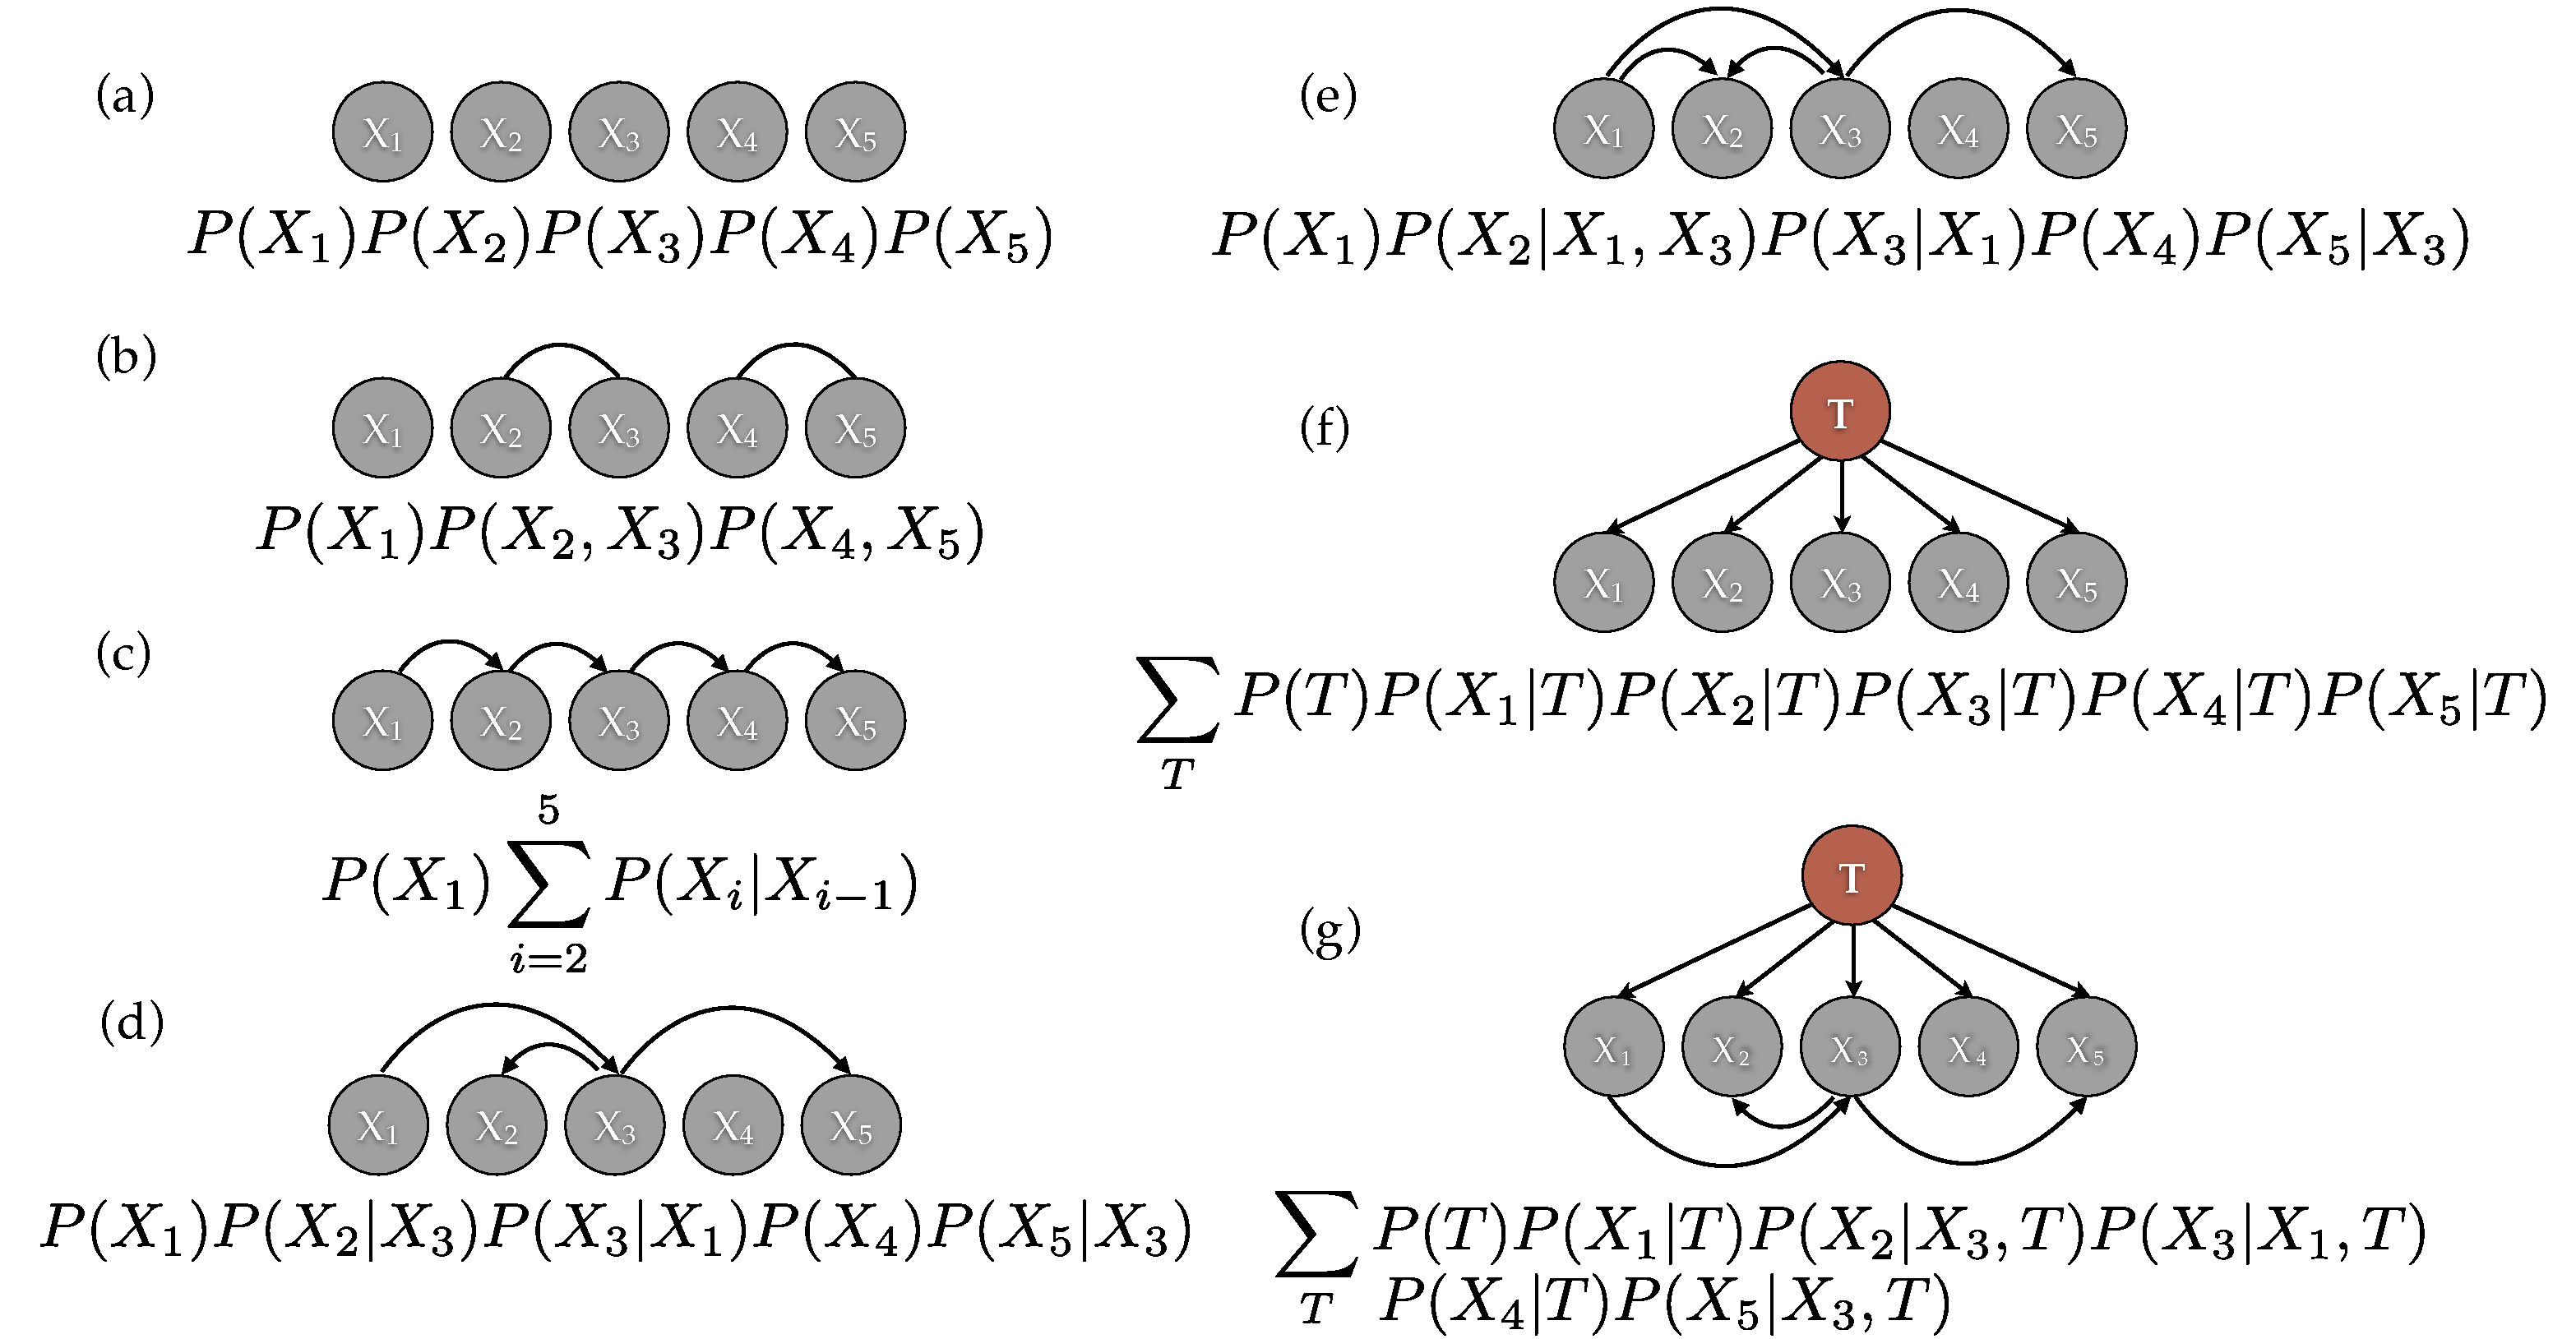
\includegraphics[width=1\textwidth]{figures/modeles-correlations.pdf}
\captionbf{Diff�rents mod�les pour d�crire les corr�lations entre nucl�otides dans les sites de fixation de \fts}{

    Figure adapt�e de \citet{Barash2003MDP} illustrant diff�rents mod�les de
    fixation sur un site de longueur $5$. Pour chaque mod�le, la structure du
    r�seau de d�pendances sous-jacent est repr�sent�e, ainsi que la
    distribution de probabilit� $P(X_1,X_2,X_3,X_4,X_5)$ correspondante, o�
    $X_i$ est une variable al�atoire prenant la valeur (A, C, G ou T) du
    nucl�otide � la position $i$.  Les mod�les repr�sent�s sont les suivants
    : (a) PWM (pas de corr�lations), (b) GWM (corr�lations mutuellement
    exclusives), (c) cha�ne de Markov d'ordre $1$ (corr�lations entre plus
    proches voisins), (d) r�seau bay�sien en arbre (au plus un parent par
    n{\oe}ud) ou (e) pas en arbre (le n{\oe}ud $2$ a deux parents), (f) m�lange
    de PWMs et (e) m�lange d'arbres � d�pendances fix�es.

}
\label{fig:modeles-correlations}
\efig

\subsection{Mod�le de r�f�rence sans corr�lations : la PWM}
\label{sub:mod_le_de_r_f_rence_sans_corr_lations_la_pwm}

Nous l'avons vu, le mod�le le plus simple (en termes de nombre de param�tres)
d�crivant l'interaction entre un TF et son site de reconnaissance sur l'ADN
consiste � faire l'hypoth�se que les nucl�otides contribuent ind�pendamment
� l'�nergie de fixation. Cette hypoth�se conduit au mod�le PWM (section
\ref{sub:modele_pwm} et fig.\ref{fig:modeles-correlations}a), qui s'�crit
\footnote{ 
    Comme nous l'avons signal� en \ref{sub:modele_pwm}, le terme PWM
    (\textit{Position Weight Matrix}) r�f�re en fait � la matrice des poids
    $\log(P(X_i)/\pi_{X_i})$ o� $\pi_{X_i}$ est une distribution neutre
    ind�pendante de la position (dite distribution \textit{background}), par exemple calcul�e
    sur des r�gions interg�niques.  
} :

\begin{equation}
    P(X_1,\cdots,X_k) = \prod_{i=1}^{K} P(X_i)
\end{equation}

o� $P(X_i)$ est la probabilit� marginale d'observer le nucl�otide $X \in
\{A,C,G,T\}$ � la position $i$. Un tel mod�le poss�de $3K$ param�tres -- $3$
param�tres $P(X_i)$ par position, la normalisation des probabilit�s permettant
de fixer le param�tre restant --. Pour une longueur de site typique $K=10$, le mod�le
PWM contient $30$ param�tres � contraindre, sachant qu'un \og mod�le \fg
complet param�trant la distribution jointe sans faire d'hypoth�se comporterait
$4^{10}-1 \sim 10^6$ param�tres.

% subsection mod_le_de_r_f_rence_sans_corr_lations_la_pwm (end)

\subsection{Une PWM g�n�ralis�e : le mod�le GWM}
\label{sub:mod_lisation_de_corr_lations_mutuellement_exclusives_le_mod_le_gwm}

 Une premi�re m�thode permettant de complexifier le mod�le PWM consiste
 � int�grer explicitement des groupes mutuellement exclusif 
 \footnote{
 Les corr�lations entre des couples de positions (i,j) et (j,k) ne peuvent �tre
 admises au sein du m�me mod�le.
 }
 de nucl�otides corr�l�s au sein du mod�le
 (fig.~\ref{fig:modeles-correlations}b). Une telle m�thode fut d'abord employ�e
 par \citet{Benos2002p3912} pour prendre en compte des corr�lations
 pr�alablement d�finies entre nucl�otides plus proches voisins. De mani�re plus
 g�n�rale, \citet{zhou2004modeling} ont d�velopp� un mod�le de matrice de poids
 g�n�ralis�e (GWM pour \textit{Generalized Weight Matrix}) qui prend en compte
 de mani�re syst�matique les corr�lations permettant d'am�liorer le mod�le
 ind�pendant. Pour ce faire, les auteurs utilisent une m�thode de Monte-Carlo
 par cha�ne de Markov (MCMC) : des corr�lations sont ajout�es ou enlev�es au
 hasard au mod�le et accept�es selon la r�gle de
 Metropolis-Hastings~\cite{krauth2006statistical}. Cette acceptation est
 proportionnelle au facteur de Bayes, une quantit� qui permet de comparer des
 mod�les poss�dant des nombres de param�tres diff�rent 
 \footnote{ 
     Sous certaines approximation, ce facteur peut se rapporter � une
     diff�rence de valeurs du BIC, introduit dans l'article en
     \ref{sec:article_maxent}. 
 } 
 .  
 Ce facteur est d�fini par le rapport entre la probabilit� de g�n�rer les
 donn�es $D$ (les s�quences de fixation) avec un mod�le $M_1$ de param�tres
 $\theta_1$ plut�t qu'avec un autre mod�le $M_2$ de param�tres $\theta_2$ :

\begin{equation}
    BF = \frac{P(D|M_1)}{P(D|M_2)} = \frac{\int P(D | \theta_1, M_1) P(\theta_1|M_1) d\theta_1}{\int P(D | \theta_2, M_2) P(\theta_2|M_2) d\theta_2}
\end{equation}

Le mod�le final consiste en un ensemble de param�tres d�crivant des positions
ind�pendantes et des positions corr�l�es mutuellement exclusives .  En analysant les donn�es TRANSFAC, les auteurs ont not� que
dans $25\%$ des cas ($22/95$) le mod�le GWM �tait significativement meilleur
que le mod�le PWM (facteur de Bayes sup�rieur � $6$). 


Cette m�thode a par la suite �t� utilis�e sur des donn�es \chipseq pour $4$ TFs
mammif�res -- NRSF, STAT$1$, CTCF et ER --~\cite{hu2010detection}. En utilisant
les $10\%$ des pics les plus importants comme ensemble d'apprentissage et en se
restreignant aux r�gions de $200$bp centr�es autour du sommet du pic \chip, les
auteurs ont r�alis� un �chantillonnage de Gibbs~\cite{casella1992explaining}
pour obtenir les sites de fixation suivant les hypoth�ses que (1) chaque pic
contient au plus un seul site de fixation (mod�le ZOOPS pour \textit{Zero or
One Occurrences Per Sequence}), (2) la probabilit� \apriori d'avoir un site
� une certaine position sur la s�quence est plus forte autour du sommet du pic,
et (3) les sites sont d�crits par un mod�le GWM.  L'�tude a r�v�l� l'existence
de corr�lations fortes limit�es aux nucl�otides plus proches voisins dans les
quatre cas �tudi�s. Les nucl�otides participant aux corr�lations se situaient
� des positions ayant un faible contenu en information dans le mod�le PWM.
Enfin, les auteurs ont not� la pr�sence de plusieurs triplets de nucl�otides
voisins corr�l�s.

% subsection mod_lisation_de_corr_lations_mutuellement_exclusives_le_mod_le_gwm (end)


\subsection{R�seaux bay�siens}
\label{sub:r_seaux_bay_siens}

Une g�n�ralisation du mod�le GWM consiste � supprimer la condition d'exclusion
mutuelle des paires de nucl�otides corr�l�s en d�crivant de mani�re plus
g�n�rale le r�seau de d�pendance entre positions. Une telle description est
possible en utilisant le langage des r�seaux bay�siens. Les d�pendances y sont
repr�sent�es par un graphe orient� acyclique \footnote{ Un graphe orient�
    acyclique est un r�seau dont les liens sont orient�s et au sein duquel il
    n'est pas possible de revenir � son point de d�part en suivant les fl�ches
} $G$, dont les n{\oe}uds sont les variables $X_i$ et les liens repr�sentent
les conditionnements d'une variable avec des variables parentes
(fig.~\ref{fig:modeles-correlations}e). La probabilit� jointe s'�crit :

\begin{equation}
    P(X_1,\cdots,X_k) = \prod_{i=1}^{K} P(X_i | P_i^G)
\end{equation}

o� $P_i^G$ est l'ensemble (pouvant �tre vide) des parents de $X_i$ dans $G$. Le
nombre de param�tres peut rapidement devenir grand : si l'on note $N_i$ le
nombre de parents de $X_i$, alors le nombre de param�tres du mod�le est $3
\sum_{i=1}^K 4^{N_i}$.

Lorsque les diff�rents n{\oe}uds poss�dent au plus un parent, on parle d'arbre
bay�sien (fig.~\ref{fig:modeles-correlations}d). Ce type de r�seau bay�sien
g�n�ralise notamment le cas des cha�nes de Markov d'ordre $1$, o� chaque
n{\oe}ud d�pend du n{\oe}ud pr�c�dent (fig.~\ref{fig:modeles-correlations}c).
Le nombre de param�tres est alors restreint, puisqu'il est au plus de
$3\cdot4K$.  \\

L'avantage des arbres bay�siens est qu'il existe des algorithmes efficaces
permettant de trouver la meilleure structure
d'arbre~\cite{friedman1997bayesian}. De tels mod�les d'arbres ont �t� utilis�s
pour d�crire les donn�es de $95$ TFs de Transfac~\cite{Barash2003MDP}. Dans
$\sim25\%$ des cas ($22/95$), le mod�le d'arbre bay�sien s'av�re
significativement meilleur qu'un mod�le PWM, ce qui est du m�me ordre de
grandeur que pour le mod�le GWM vu
en~\ref{sub:mod_lisation_de_corr_lations_mutuellement_exclusives_le_mod_le_gwm}.


% subsection r_seaux_bay_siens (end)

\subsection{Mod�les de m�lange}
\label{sub:mod_les_de_m_lange}

Dans les cas pr�c�dents, nous avons pr�sent� des mod�les capturant des
d�pendances \og locales \fg entre paires de nucl�otides. N�anmoins, il peut
exister des d�pendances plus largement r�parties entre les positions, comme
cela a d�j� �t� observ� empiriquement~\cite{Badis2009p3911,Jolma2013p3971}. De
telles corr�lations � plus grande �chelle peuvent �tre mod�lis�es en supposant
que le \tf poss�de plusieurs \og modes \fg de fixation. Ceux-ci peuvent par
exemple correspondre � diff�rentes conformations de la prot�ine sur son site de
fixation, chaque configuration poss�dant ses propres pr�f�rences de fixation.
Ces modes sont d�crits par une variable al�atoire $T$ (le \textit{type} de
fixation) de probabilit� $P(T)$. Il est ensuite possible de d�crire la fixation
au sein de chaque mode par l'un des mod�les pr�c�dents.

\subsubsection{M�lange de PWMs}
\label{ssub:m_lange_de_pwms}

Le cas le plus naturel consiste � utiliser comme mod�le de fixation le mod�le
PWM, \cad que dans chaque mode il y a ind�pendance entre les positions. La
probabilit� d'observer un site est alors donn�e par la somme sur les diff�rents
modes de fixation de la probabilit� de fixer un site, conditionn�e par la
probabilit� d'�tre dans ce mode :

\begin{equation}
    P(X_1,\cdots,X_K) = \sum_{T=1}^N P(T) \prod_{i=1}^K P(X_i|T)
\end{equation}

o� $N$ est le nombre de modes de fixation. Ce mod�le a plusieurs avantages.
D'abord, le nombre de param�tres reste lin�aire en $K$ : pour d�crire $P(T)$ et
les $N$ PWMs il faut $N - 1 + 3KN$ param�tres. Ce nombre reste dont
raisonnablement faible devant le nombre de param�tres requis pour compl�tement
d�crire les interactions � deux nucl�otides, qui cro�t comme $K^2$. Ensuite, le
mod�le a une interpr�tation claire qui peut permettre de mettre en exergue un
m�canisme biologique sous-jacent.  \\

Ce type de mod�le permet de d�passer le mod�le PWM dans un nombre substantiel
de cas. Ainsi, \citet{Barash2003MDP} ont montr� que $\sim40\%$ des TFs de
Transfac ($36/95$) sont significativement mieux repr�sent�s par un m�lange de
$2$ PWMs que par une seule PWM. En utilisant des donn�es \invitro plus pr�cises
pour $104$ TFs de la souris, \citet{Badis2009p3911} ont montr� que $\sim 85\%$
($89/104$) �taient mieux repr�sent� par une combinaison de PWMs que par une PWM
seule, plaidant pour un port�e g�n�rale de l'existence de \og motifs
secondaires \fg.


% subsubsection m_lange_de_pwms (end)


\subsubsection{M�lange d'arbres}
\label{ssub:m_lange_d_abres}

De la m�me mani�re que les PWMs, il est possible d'�tendre les mod�les d'arbres
en r�alisant un m�lange d'arbres. Intuitivement, ceci permet de capturer des
d�pendances additionnelles en gardant un nombre de param�tres lin�aire en
fonction de la taille du motif. Un tel mod�le semble poss�der des performances
comparables au m�lange de PWM, et am�liore la description des TFs de Transfac
dans $\sim40\%$ des cas ($35/95$)~\cite{Barash2003MDP}.


% subsubsection m_lange_d_abres (end)


% subsection mod_les_de_m_lange (end)

\section{Mod�les de maximum d'entropie}
\label{sec:modeles-maxent}

\bfig
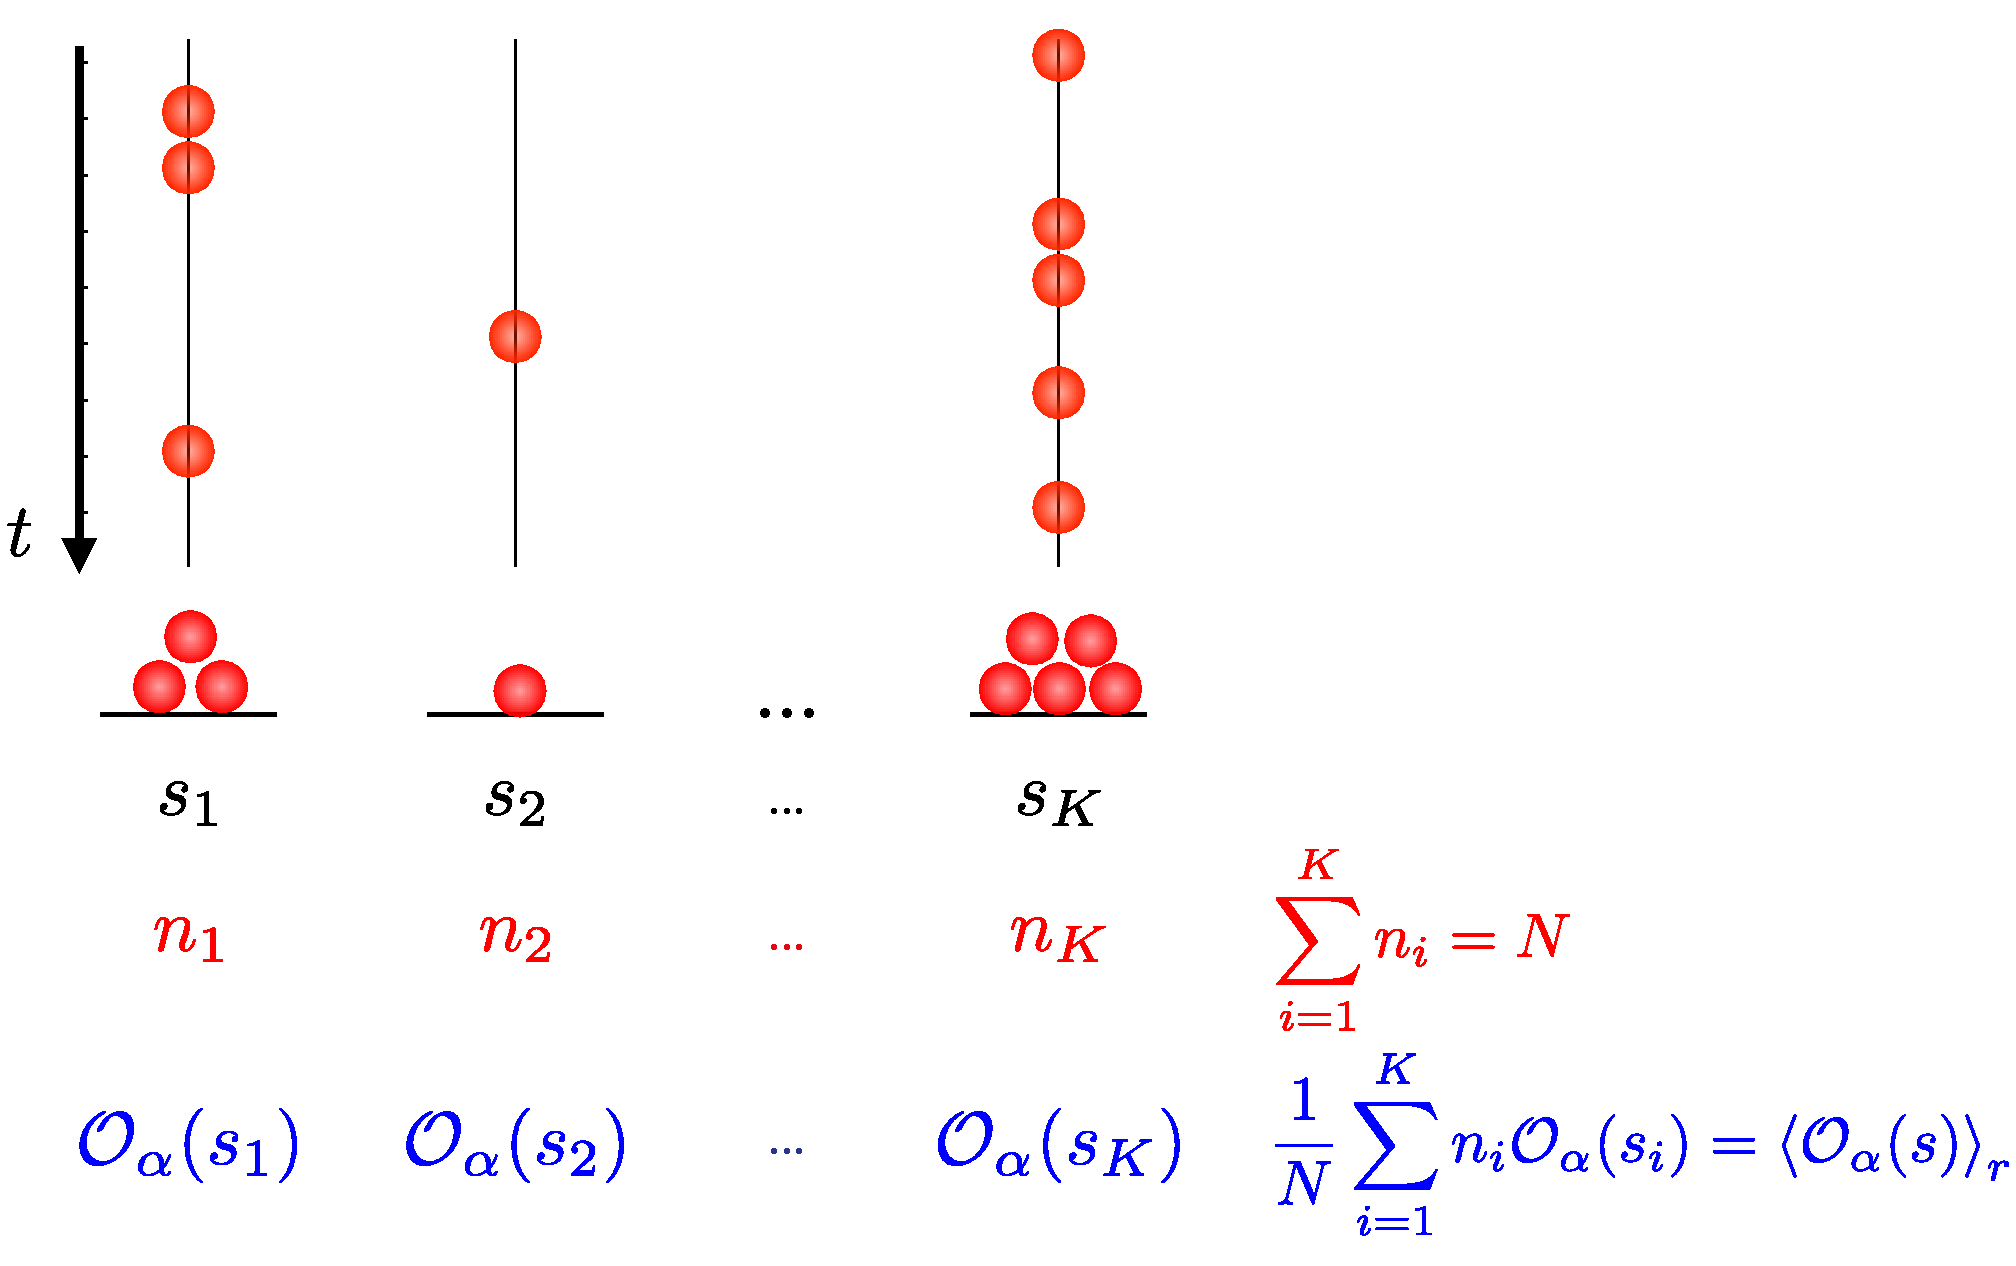
\includegraphics[width=1.0\textwidth]{figures/entropie.pdf}
\captionbf{Illustration d'un syst�me dont on veut maximiser l'entropie}{

    Le syst�me explore $K$ �tats $\{s_1,\cdots,s_K\}$ au cours du temps. Au
    bout de $N$ observations, un �tat $s_i$ a �t� observ� $n_i$ fois. � chaque
    �tat correspond un certain nombre de quantit�s $\mathcal{O}_\alpha(s_i)$
    dont seule la valeur moyenne empirique $\left\langle
    \mathcal{O}_\alpha(s)\right\rangle_r$ est connue de l'observateur (on parle
    d'\og observable \fg).

}
\label{fig:entropie}
\efig


\subsection{Pourquoi maximiser l'entropie?}
\label{sub:pourquoi_maximiser_l_entropie_}

Le concept d'entropie remonte aux pr�misses de la physique
statistique~\cite{Jaynes1978p795}. Dans l'essence, il peut �tre compris de la
mani�re suivante. Supposons qu'un syst�me comporte $K$ �tats distincts
$\{s_1,\cdots,s_K\}$. Au cours du temps, le syst�me explore les diff�rents
�tats (fig.~\ref{fig:entropie}). Au bout de $N$ observations, chaque �tat a �t�
observ� un nombre $n_i$ de fois. La question sous-jacente au calcul de
l'entropie est la suivante : sans connaissance \apriori sur le syst�me, que
puis-je dire de ces $n_i$? Prenons l'exemple de la figure \ref{fig:entropie}.
On a certaines valeurs pour les $n_i$ ($n_1=3$, $n_2=1$, etc.), et on aimerait
savoir de combien de mani�res il est possible de r�aliser un tel ensemble de
valeurs. Notons ce nombre $\mathcal{N}(n_1,\cdots,n_K)$. Il est donn� par la
formule suivante :

\begin{align}
    \begin{split}
    \mathcal{N}(n_1,\cdots,n_K) & = \binom{N}{n_1}\binom{N-n_1}{n_2}\cdots\binom{N-\sum_{i=1}^{K-1} n_i}{n_K} \\
    & = \frac{N!}{(N-n_1)!n_1!} \times \frac{(N-n_1)!}{(N-n_1-n_2)!n_2!} \times \cdots \times \frac{(N-\sum_{i=1}^{K-1}n_i)!}{0!n_K!}
    \end{split}
\end{align}

soit

\begin{equation}
   \mathcal{N}(n_1,\cdots,n_K) = \frac{N!}{n_1!n_2!\cdots n_K!} 
\end{equation}    

Il convient alors de s'int�resser au logarithme de cette quantit�. En effet, dans le cas o� les nombres d'observation sont grands $n_i \gg 1$, ceux-ci s'expriment simplement gr�ce � la formule de Stirling :

\begin{equation}
    \log(n!) \xrightarrow[n\to\infty]{} n\log(n)-n
\end{equation}

On peut alors �crire

\begin{align}
    \begin{split}
   \log\mathcal{N}(n_1,\cdots,n_K) & = N\log(N) - N - \sum_{i=1}^K \left(n_i\log(n_i) -n_i\right) \\ 
   & = \sum_{i=1}^K n_i\log(\frac{N}{n_i}) \\ 
   & = -N \sum_{i=1}^K \frac{n_i}{N}\log(\frac{n_i}{N})
   \end{split}
\end{align}

On note l'apparition des probabilit�s empiriques $f(s_i)=n_i/N$ d'observer
l'�tat $s_i$, qui tendent asymptotiquement (dans la limite \og thermodynamique \fg
$N \to \infty$) vers les \og vraies \fg probabilit�s $P(s_i)$. L'entropie est d�finie dans cette limite comme �tant �gale � $1/N\log\mathcal{N}(n_1,\cdots,n_K)$, soit

\begin{equation}
   \label{eq-entropy}
   \boxed{
   S[P] = - \sum_{\left\{ s \right\}}P(s) \log P(s)
   }
\end{equation}

o� $\{s\} = \{s_1,\cdots,s_K\}$ d�note l'ensemble des �tats accessibles. L'id�e
est alors la suivante : nous souhaitons savoir quels �tats le syst�me a le plus
probablement visit� au cours des $N$ transitions. Sans connaissance \apriori
sur le syst�me, il est plus probable que les nombres $(n_1,\cdots,n_K)$ obtenus
soient ceux qui sont r�alis�s le plus souvent, \cad ceux qui maximisent la
quantit� $\mathcal{N}(n_1,\cdots,n_K)$ et donc au final l'entropie. Par
ailleurs, les fluctuations relatives des quantit�s $n_i$ sont de l'ordre de
$1/\sqrt{n_i}$~\cite{sethna2006statistical}.  Ainsi, la solution de maximum
d'entropie domine largement les autres solutions possibles dans la limite
thermodynamique.

% subsection pourquoi_maximiser_l_entropie_ (end)

\subsection{Maximisation de l'entropie sous contraintes}
\label{sub:maximisation_de_l_entropie_sous_contraintes}

Notons $\mathcal{O}_\al(s)$ une quantit� attach�e � $s$
(fig.~\ref{fig:entropie}). En thermodynamique, une telle quantit� correspond
par exemple � l'�nergie d'un �tat. L'observateur n'a lui acc�s qu'aux valeurs
moyennes de telles quantit�s sous-jacentes. � l'�tat d'�quilibre
thermodynamique, l'�chantillonnage des �tats est r�alis� au sein de la
distribution de probabilit� de maximum d'entropie $P(s)$, et les valeurs
moyennes calcul�es avec les fr�quences empiriques $f(s)$ doivent donc �tre
compatibles avec les valeurs moyennes calcul�es avec la distribution de
probabilit� $P(s)$ :

\begin{equation}
   \label{eq:constraints}
   \sum_{\{s\}} P(s) \mathcal{O}_\al(s) = \sum_{\{s\}}f(s) \mathcal{O}_\al(s)
\end{equation}

Nous souhaiterions maintenant conna�tre la distribution $P(s)$ la moins biais�e
(i.e de maximum d'entropie) qui satisfait les contraintes de l'�q.
\ref{eq:constraints} impos�es par l'observation des donn�es (l'information que
poss�de l'observateur). Ce probl�me revient � maximiser le Lagrangien suivant :

\begin{equation}
   \mathcal{L}  =  - \sum_{\{ s \}} P(s) \log P(s) + \lambda \left(\sum_{\{ s \}}
   P(s) -1\right)  +  \sum_\al \beta_\al \sum_{\{s\}} \left( P(s) - f(s) \right) \mathcal{O}_\al(s) 
\end{equation}

o� les param�tres $\lambda$ et $\beta_\al$ sont les multiplicateurs de Lagrange
correspondant respectivement � la contrainte de normalisation de la
distribution de probabilit� et aux informations qu'a l'observateur sur
certaines valeurs moyennes du syst�me (�q. \ref{eq:constraints}).  La
maximisation de ce Lagrangien est obtenue en annulant la d�riv�e fonctionnelle
par rapport � la distribution de probabilit� $P(s)$ :

\begin{equation}
   \frac{\delta \mathcal{L}}{\delta  P(s)}   =  0  
   = - \ln P(s) - 1  + \lambda  
   +  \sum_{\al} \beta_\al \mathcal{O}_\al(s)
\end{equation}

En utilisant la normalisation des probabilit�s, il est possible de trouver
$\lambda$, et la solution se met finalement sous la forme 

\begin{equation}
    \label{eq:boltzmann}
    \boxed{
        P(s) = \frac{1}{\mathcal{Z}} e^{-\mathcal{H}(s)}
    }
\end{equation}

o� $\mathcal{H}$ est l'Hamiltonien du syst�me :

\begin{equation}
   \mathcal{H} = \sum_\al \beta_\al\mathcal{O}_\al(s)
\end{equation}

et $\mathcal{Z}$ est la fonction de partition permettant la normalisation de la
distribution $P(s)$ :

\begin{equation}
   \mathcal{Z}=\sum_{\{s\}} \exp[- \mathcal{H}(s)].
\end{equation}


\Remarque{

    \footnotesize{ Il est possible de montrer que la maximisation de
        l'entropie, partant des contraintes de l'�q. \ref{eq:constraints} sur
        les valeurs moyennes pour en arriver � une forme exponentielle de la
        distribution de probabilit�, est le contrepoint d'une maximisation de
        la vraisemblance partant d'une forme exponentielle pour en arriver aux
        m�mes contraintes sur les valeurs
        moyennes~\cite{grendar2001minimax,jaynes1982rationale}.  }

}

% subsection maximisation_de_l_entropie_sous_contraintes (end)

\subsection{Application aux sites de fixation}
\label{sub:application_aux_sites_de_fixation}

\subsubsection{Corr�lations � un point : le mod�le PWM}
\label{ssub:corr_lation_un_point_le_mod_le_pwm}

Dans le cas qui nous int�resse, un �tat $s$ correspond � une s�quence d'ADN
appartenant � l'ensemble $\left\{ s \right\}$ des sites de fixation d'un \tf.
Consid�rons maintenant l'observable quantifiant la pr�sence du nucl�otide $a$
� la position $i$ d'un site :

\begin{equation}
    \mathcal{O}_{i,a}(s) = \delta(s_i,a)
\end{equation}


o� $\delta$ est la fonction de Kronecker qui vaut $1$ lorsque le nucl�otide
� la position $i$ du site $s_i$ vaut $a$ et $0$ sinon. De cette d�finition il suit que la valeur moyenne sur les fr�quences empiriques


\begin{equation}
    \label{eq:onepoint}
    \sum_{\{s\}} f(s) \mathcal{O}_{i,a}(s) = f_{i,a}
\end{equation}

se r�duit � la fr�quence du nucl�otide $a$ � la position $i$. Notons $h_i(a)$
le multiplicateur de Lagrange correspondant et $\mathcal{A} = \{A,C,G,T\}$. On trouve alors

\begin{align}
    \begin{split}
    \mathcal{H}(s) & = \sum_{i=1}^L \sum_{a \in \mathcal{A}} h_i(a) \delta(s_i,a)\\
     & = \sum_{i=1}^L h_{i}(s_i)
    \end{split}
\end{align}

Les diff�rentes positions �tant ind�pendantes, la fonction de partition
$\mathcal{Z}$ peut par ailleurs se scinder en diff�rentes fonctions de partition par
position : $\mathcal{Z}=\prod_{i=1}^L\mathcal{Z}_i$. On obtient au final

\begin{equation}
    P(s) = \frac{1}{\mathcal{Z}} e^{-\sum\limits_{i=1}^L h_i(s_i)} = \prod_{i=1}^L \frac{e^{-h_i(s_i)}}{\mathcal{Z}_i}
\end{equation}

On retrouve le mod�le PWM introduit dans l'�q.~\ref{eq:boltzmann}.



% subsubsection corr_lation_un_point_le_mod_le_pwm (end)

\subsubsection{Corr�lations � deux points : le mod�le de Potts}
\label{ssub:corr_lations_deux_points_le_mod_le_de_potts}


Il est maintenant relativement direct de complexifier le mod�le en ajoutant
l'observation des couples d'interaction au sein des sites de fixation :

\begin{equation}
    \mathcal{O}_{i,a,j,b}(s) = \delta(s_i,a)\delta(s_j,b)
\end{equation}

La corr�lation � deux points entre le nucl�otide $a$ en position $i$ et $b$ en
position $j$ s'�crit donc 

\begin{equation}
    \label{eq:twopoints}
    \sum_{\{s\}} f(s) \mathcal{O}_{i,a,j,b}(s) = f_{i,a,j,b}
\end{equation}

o� $f_{i,a,j,b}$ est la fr�quence empirique d'observation de la paire de
nucl�otide $(a,b)$ aux positions $(i,j)$. Notons $J_{i,j}(a,b)$ le
multiplicateur de Lagrange correspondant. L'Hamiltonien sous les contraintes
impos�es par les �quations \ref{eq:onepoint} et \ref{eq:twopoints} s'�crit :


\begin{align}
    \begin{split}
    \mathcal{H}(s) & = \sum_{i=1}^L \sum_{a \in \mathcal{A}} h_i(a) \delta(s_i,a) + \sum_{i=1}^{L-1} \sum_{j>i} \sum_{a \in \mathcal{A}} \sum_{b \in \mathcal{A}} J_{i,j}(a,b) \delta(s_i,a)\delta(s_j,b)\\
    & = \sum_{i=1}^L h_{i}(s_i) + \sum_{i=1}^{L-1}\sum_{j>i} J_{i,j}(s_i,s_j)
\end{split}
\end{align}

Le mod�le de maximum d'entropie est finalement

\begin{equation}
    \label{eq:potts}
    \boxed{
    P(s) = \frac{1}{\mathcal{Z}} e^{-\sum\limits_{i=1}^L h_i(s_i)-\sum\limits_{i=1}^{L-1} \sum\limits_{j>i} J_{i,j}(s_i,s_j)} 
}
\end{equation}

On reconna�t le mod�le de Potts inhomog�ne de champs magn�tiques locaux $h_i$
et de termes d'interaction $J_{i,j}$ couramment utilis� dans la description des
verres de spins~\cite{baxter2007exactly}.


% subsubsection corr_lations_deux_points_le_mod_le_de_potts (end)

% subsection application_aux_sites_de_fixation (end)


\section{Article} 
\label{sec:article_maxent}

L'article qui suit d�crit l'analyse de donn�es de fixation \invivo � grande �chelle
pour plusieurs TFs drosophiles et mammif�res. Diff�rents mod�les sont compar�s,
incluant ou non des d�pendances : un mod�le PWM, un mod�le de m�lange de PWMs,
et un mod�le de Potts.


%\includepdf[pages=-]{articles/maxent-arxiv}

% section article (end)


\section{Analyse thermodynamique des mod�les} 
\label{sec:analyse_thermodynamique_des_mod_les_ind_pendant_et_avec_couplages}
\subsection{Chaleur sp�cifique}
\label{sub:chaleur_sp_cifique}


En plus des r�sultats pr�sent�s dans l'article, nous nous sommes int�ress�s
� une quantit� classique de la thermodynamique : la chaleur sp�cifique ou
capacit� calorifique. Consid�rons un mod�le d�crit par la statistique de
Boltzmann � la temp�rature inverse $\beta=1/T$ (on omet la constante de
Boltzmann $k$ en l'int�grant � l'�nergie):

\begin{equation}
    \label{eq:boltzmann_with_beta}
    P(s) = \frac{1}{\mathcal{Z}} e^{-\beta E(s)}
\end{equation}

Le cas de l'�quation \ref{eq:potts} correspond au cas particulier $\beta=1$.
Nous voulons voir comment l'amplification ou la diminution globale de l'�cart
entre les �nergies affecte la possibilit� du syst�me d'explorer les diff�rents
�tats possibles. � temp�rature nulle ($T\to0 $ ou $\beta \to \infty$), le
syst�me reste dans le niveau fondamental de minimum d'�nergie et de probabilit�
$1$, alors qu'� des temp�ratures non nulles le syst�me � l'�nergie $E_0$
transite vers un �tat d'�nergie sup�rieure $E_1$ avec une probabilit� $\propto
\exp\left(-\beta (E_1-E_0)\right)$. Lorsqu'un paysage �nerg�tique est compos�
de plusieurs puits d'�nergie s�par�s par des barri�res �nerg�tiques
importantes, on s'attend � avoir une (ou plusieurs) temp�ratures critiques
� partir desquelles de fortes diff�rences d'�nergie deviennent franchissables.
L'�nergie moyenne peut alors �tre significativement affect�e, sautant
soudainement � une nouvelle valeur du fait du poids des nouveaux �tats
explor�s. 

La chaleur sp�cifique permet de caract�riser ces sauts soudains d'�nergie
moyenne lors de la variation de la temp�rature, caract�ristiques des
transitions de phase. Elle mesure simplement la variation de l'�nergie moyenne
lors d'une variation de temp�rature :

\begin{equation}
    C(T) = \frac{d\langle E \rangle}{dT}
\end{equation}

o� 

\begin{equation}
    \langle E \rangle = \sum_{\{s\}} E(s) \frac{e^{-\beta E(s)}}{\mathcal{Z}}
\end{equation}

Cette chaleur sp�cifique peut par ailleurs s'�crire sous une forme plus utile : 

\begin{align}
    \label{eq:fluctuation-dissipation}
    \begin{split}
        \frac{d\langle E \rangle}{dT} & = - \beta^2 \frac{d\langle E \rangle}{d\beta} \\
        & = - \beta^2 \left[\sum_{\{s\}} E(s) \left( -E(s) e^{-\beta E(s)} \right)\frac{1}{\mathcal{Z}} + \sum_{\{s\}} E(s) e^{-\beta(E(s))} \left(-\frac{d\mathcal{Z}}{d\beta} \frac{1}{\mathcal{Z}^2}\right)\right] \\
    & = \beta^2 \left[ \langle {E}^2 \rangle - {\langle E \rangle}^2 \right]
    \end{split}
\end{align}

Ainsi, la chaleur sp�cifique $C(T)$ est directement accessible en regardant les
corr�lations de l'�nergie sur l'ensemble des �tats du syst�me, ce qui peut se
calculer simplement � partir des mod�les de fixation.  Nous avons calcul� la
variation de $C(T)$ en fonction de la temp�rature pour les mod�les ind�pendant
et avec d�pendances obtenus en \ref{sec:article_maxent} pour les diff�rents TFs
�tudi�s. Une temp�rature fictive est introduite dans les mod�les en multipliant
les �nergies par $\beta$, afin de se placer dans le cadre de l'�quation
\ref{eq:boltzmann_with_beta}. Les r�sultats sont montr�s en
figure~\ref{fig:maxent/specific_heat} (mod�le ind�pendant en bleu, mod�le de
Potts en rouge). On observe pour la plupart des facteurs l'existence de deux
pics de chaleur sp�cifique pour des temp�ratures de l'ordre de $T\sim10^{-1}$
et $T\sim 5$ (par exemple, $T=0.4$ et $T=2.8$ dans le cas du mod�le ind�pendant
de Twist). Il y a de l�g�res variations entre les deux mod�les : notamment, le
premier pic semble renforc� par le mod�le de Potts dans plusieurs cas (par
exemple, E$2$f$4$, NRSF, TCF$3$ ou Twist). N�anmoins, le nombre de pics (ou de
transitions de phases) reste le m�me.

\bfig
\includegraphics[width=0.8\textwidth]{figures/maxent/specific_heat.pdf}
\captionbf{Chaleur sp�cifique pour diff�rents TFs}{

    La chaleur sp�cifique (l'�quivalent de la capacit� calorifique en
    thermodynamique) $C(T)=d\langle E\rangle/dT$ est trac�e en fonction de la
    temp�rature $kT$ (�chelle logarithmique) pour les diff�rents TFs
    consid�r�s. Le mod�le ind�pendant (bleu) et le mod�le de Potts avec
    interactions (rouge) sont comparables dans la plupart des cas.

}
\label{fig:maxent/specific_heat}
\efig

% subsection chaleur_sp_cifique (end)

\subsection{Lien avec les valeurs des champs et des couplages}
\label{sub:lien_avec_les_valeurs_des_champs_et_des_couplages}

Afin de comprendre l'existence des pics de chaleur sp�cifique et les �nergies
(temp�ratures) associ�es, il faut revenir aux mod�les d'�nergie. Lorsque l'on
regarde l'histogramme des valeurs absolues de $h_i$ obtenues dans les mod�les
ind�pendant des diff�rents TFs �tudi�s, on trouve plusieurs valeurs typiques
autour de $10^{-4}$, $1$ et $10$ (fig.~\ref{fig:histogrammes_champs}A).
Celles-ci peuvent s'expliquer de la mani�re suivante. Dans le mod�le
ind�pendant, les champs sont simplement le logarithme naturel de la probabilit�
d'observer un nucl�otide $a$ � une position $i$ donn�e $h_i(a) = -\log P_i(a)$
(la jauge est choisie telle que $\mathcal{Z_i}=1$). En valeur absolue, les
champs $h_i$ proches de $0$ ($h_i\sim10^{-4}-10^{-3}$) correspondent aux
nucl�otides tr�s conserv�s (toujours observ�s), les valeurs autour de $1$
correspondent � des nucl�otides d�g�n�r�s (i.e �galement observ�s
: $|\log(1/4)| \sim 1.4$) et les valeurs autour de $10$ correspondent aux
nucl�otides qui ne sont jamais observ�s, au pseudocount pr�s (pour un
pseudocount de $1$ et $10^4$ s�quences, $|\log(10^{-4})| \sim 9.2$).  On peut
maintenant mieux comprendre les pics de chaleur sp�cifique. � temp�rature
nulle, seuls les sites consensus sont accessibles. Lorsque la temp�rature se
rapproche de $1$, les nucl�otides d�g�n�r�s d'�nergie $h_i\sim1$ deviennent
accessibles, augmentant significativement la valeur de l'�nergie moyenne
(premier pic). Puis, lorsque la temp�rature se rapproche de $10$, les
nucl�otides non observ�s d'�nergie $h_i\sim10$ deviennent � leur tour
accessibles, augmentant � nouveau l'�nergie moyenne (deuxi�me pic).

Dans le cas du mod�le de Potts (fig.~\ref{fig:histogrammes_champs}B), les
champs $h_i$ prennent des valeurs proches de celles obtenues avec le mod�le
ind�pendant. Par ailleurs, les interactions $J_{i,j}$ sont r�parties autour
d'un mode centr� autour de $J_{i,j} \sim 0.5$, ce qui correspond l'�chelle
d'�nergie du premier pic. Ainsi, le renforcement du premier pic de chaleur
sp�cifique par rapport au cas ind�pendant observ� pour plusieurs TFs de la
figure \ref{fig:maxent/specific_heat} peut s'expliquer par l'effet des termes
d'interaction $J_{i,j}$.


\bfig
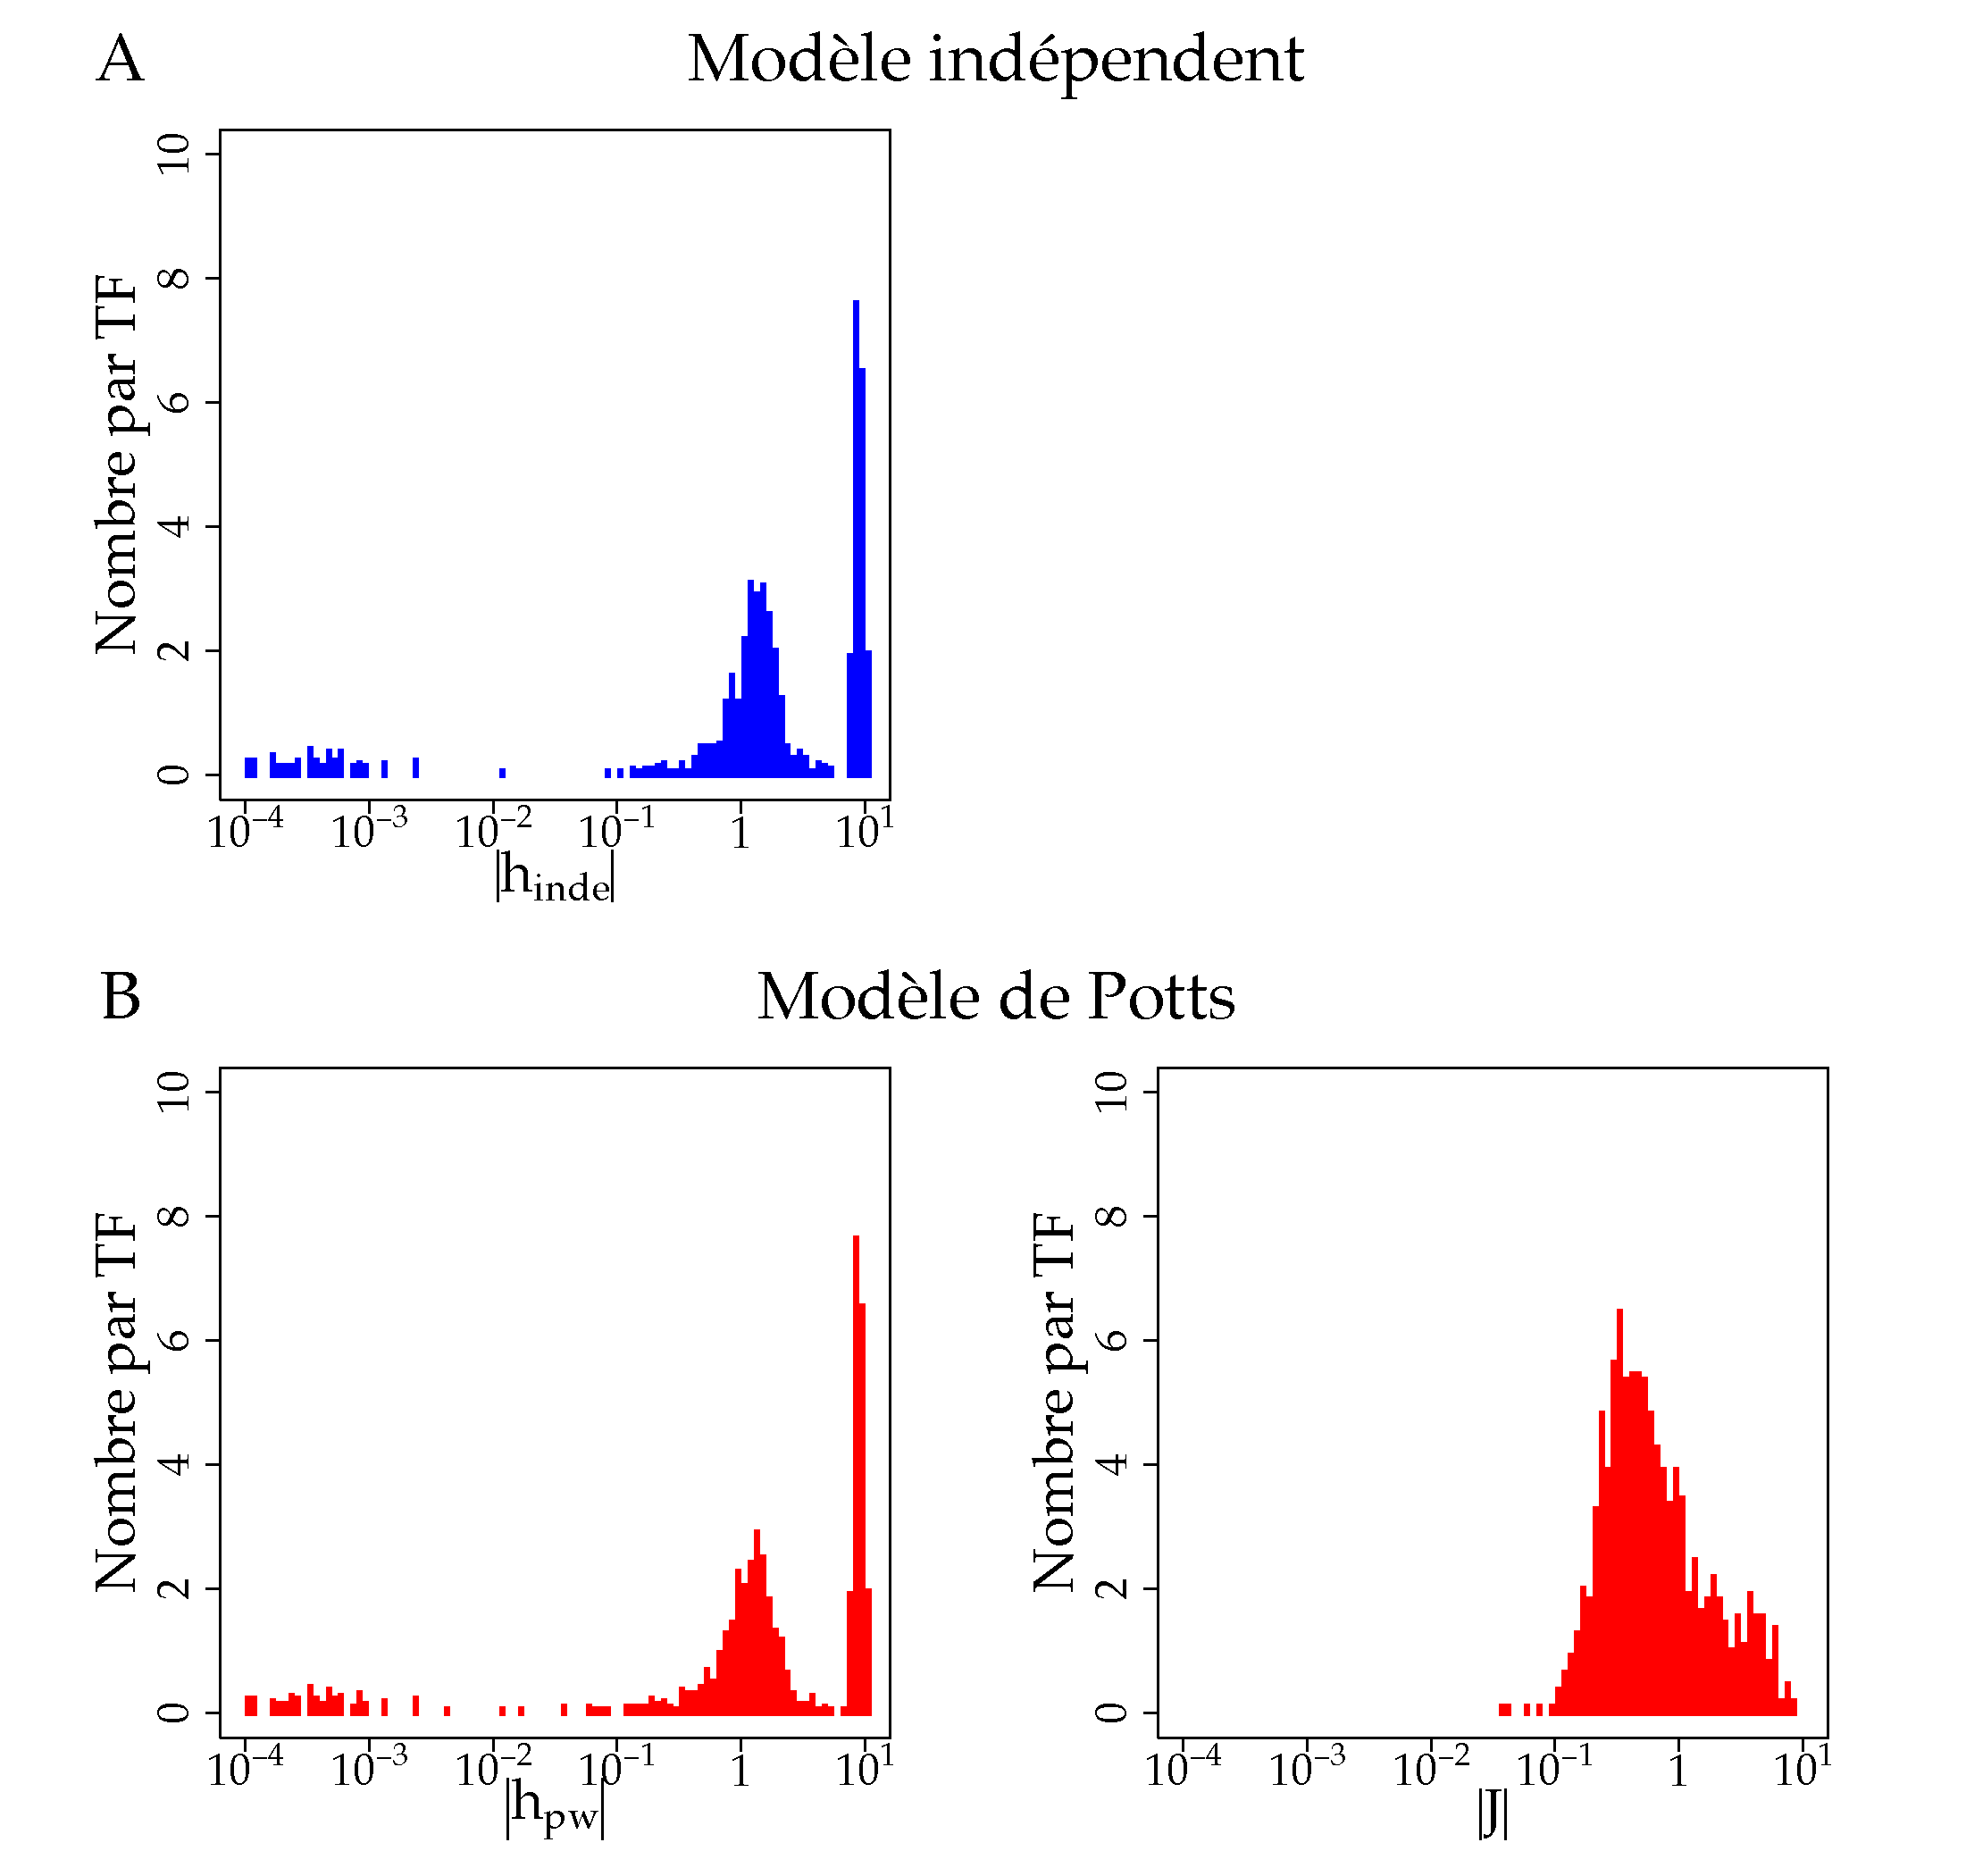
\includegraphics[width=1.\textwidth]{figures/maxent/histogrammes_champs.pdf}
\captionbf{Histogrammes des valeurs des champs $h$ et couplages $J$}{

    Histogrammes r�alis�s � partir des valeurs obtenues pour l'ensemble des
    TFs. Les champs et les couplages sont montr�s en valeur absolue sur une
    �chelle logarithmique d'espacement $0.05$, et les valeurs nulles ne sont
    pas repr�sent�es. (A) Champs $h_{inde}$ dans le mod�le ind�pendant. (B)
    Champs $h_{pw}$ et couplages $J$ dans le mod�le de Potts.

}
\label{fig:histogrammes_champs}
\efig


% subsection lien_avec_les_valeurs_des_champs_et_des_couplages (end)

% section analyse_thermodynamique_des_mod_les_ind_pendant_et_avec_couplages (end)
\section{Conclusion et perspectives}


Nous avons analys� les d�pendances au sein des sites de fixation li�s \invivo
pour diff�rents \tfs Drosophiles et mammif�res. Nous avons compar� les
performances d'un mod�le PWM, d'un mod�le de m�lange de PWMs, et d'un mod�le de
Potts, en utilisant un crit�re bay�sien (BIC) p�nalisant les mod�les � grand
nombre de param�tres. Nous avons exhib� l'existence de corr�lations faibles
dont la prise en compte permet de significativement am�liorer la description
des donn�es, le mod�le de Potts �tant significativement sup�rieur aux deux
autres mod�les dans la plupart des cas ($22/28$). Les interactions ont �t�
�tudi�es syst�matiquement, montrant notamment une pr�pond�rance des
interactions entre plus proches voisins. Nous avons �tabli une correspondance
entre les PWMs du mod�le de m�lange et les PWMs d�crivant les �tats
m�tastables du paysage �nerg�tique g�n�r� par le mod�le de Potts. Enfin, nous
avons montr� que les corr�lations pouvaient �tre group�es en patterns de
Hopfield ou \og m�moires \fg, et qu'un petit nombre �tait suffisant
� reconstruire le paysage d'interactions.  \\

Une perspective int�ressante de ce travail serait de conduire la m�me analyse
sur des donn�es grande �chelle obtenues \invitro par la m�thode
HT-SELEX~\cite{Jolma2013p3971}. Notamment, certains des facteurs que nous avons
�tudi�s \invivo sont repr�sent�s dans ces donn�es, et il serait int�ressant de
voir les diff�rences entre les mod�les obtenus. Notamment, retrouve-t-on les
m�mes corr�lations? Peut-on exhiber des sp�cificit�s de la fixation \invivo, o�
l'on s'attend � avoir des effets provenant de diverses sources (fixation de
nucl�osomes, superposition de sites de fixations, \ldots)? Ces questions feront
certainement l'objet d'un prochain travail.



\newpage

%%%%%%%%%%%%%%%%%%%%%%%%%%%%%%%%%%%%%%%%%%%%%%%%%%%%%%%%%%%%%%%%%%%%%%%%%%%%%%%%%%%%%%%%%%
\chapter{\ChImogene} 
\label{ch:imogene}
%\adjustmtc
\minitoc
\newpage
\section*{Introduction du chapitre \thechapter}

Dans le chapitre \ref{ch:maxent}, nous avons vu comment d�crire l'interaction
TF-ADN lorsque des sites de fixation sont connus. Dans ce chapitre, nous
adoptons une d�marche plus g�n�rale. Nous connaissons l'activit� de r�gulation
d'un certain nombre de CRMs, et nous souhaitons savoir quels TFs s'y fixent
(recherche de motifs), et si le g�nome contient d'autres CRMs avec la m�me
activit� (recherche de modules). Un algorithme permettant pr�cis�ment de
r�aliser ces �tapes a �t� d�velopp� pr�c�demment par Herv� Rouault et appliqu�
au cas de la diff�renciation des organes sensoriels de la
Drosophile~\cite{Rouault2010p327}. Nous pr�sentons ici Imogene, l'extension de
cet algorithme au cas des mammif�res, ainsi que son utilisation comme outil de
classification de CRMs associ�s � diff�rentes r�gulations.

Avant de rentrer dans le d�tail d'Imogene, nous pr�sentons les m�thodes
existantes de recherche de motifs dans des CRMs. Le probl�me g�n�ral est le
suivant : �tant donn�es des CRMs conduisant � une m�me r�gulation (l'ensemble
d'apprentissage), peut-on construire des mod�les de sites de fixation qui \og
expliquent \fg cette co-r�gulation, \cad qui pr�disent l'existence de sites sur
les CRMs mais pas sur des s�quences ne participant pas � la cor�gulation?



\section{Les approches existantes pour la recherche de motifs et de modules de r�gulation} 
\label{sec:approches_existantes}

Nous avons d�j� introduit diff�rentes m�thodes de pr�diction de motifs et
modules en introduction (section \ref{sec:prediction_crms}). Ici nous d�crivons
plus en avant certaines approches. Pour une revue plus exhaustive, le lecteur
int�ress� pourra se r�f�rer � \citet{Aerts2012p3868}.

\subsection{MEME : une approche de type Esp�rance-Maximisation}
\label{sub:meme_une_approche_de_type_esp_rance_maximisation}

L'une des premi�res approches pour la pr�diction \denovo de motifs � partir de
s�quences a �t� celle de MEME~\cite{Bailey1994fk}, un algorithme bas� sur la
m�thode d'esp�rance-maximisation ou EM (\textit{expectation maximization})
utilis�e pr�c�demment dans ce cadre par \citet{Lawrence1990uq}. Cet algorithme
se base sur une approche g�n�rative pour d�crire les processus probabilistes
qui ont permis la g�n�ration des s�quences CRMs
(fig.~\ref{fig:d_haeseleer-MEME}). 

\bfig
\includegraphics[width=0.8\textwidth]{figures/d_haeseleer-MEME.pdf}
\captionbf{Illustration de l'approche esp�rance-maximisation}{

Figure tir�e de \cite{Dhaeseleer2006kx} d�crivant l'approche EM. Un premier
mod�le de motif est construit � partir d'un site initial. Ce mod�le permet de
pond�rer l'ensemble de sites sur les s�quences (�tape E). En rouge sont montr�s
les meilleurs sites pour chaque s�quence. En utilisant ces poids, il est
possible de construire un mod�le de vraisemblance maximale (�tape M). La
m�thode originale de \citet{Lawrence1990uq} fait l'hypoth�se qu'il
y a exactement un site de fixation par s�quence, condition qui est rel�ch�e par
MEME. 

} \label{fig:d_haeseleer-MEME} \efig


\subsubsection{Vraisemblance d'une s�quence}
\label{ssub:vraisemblance_d_une_s_quence}


Notons $S=\{S_1,\cdots,S_L\}$ une s�quence de taille $L$.\footnote{On concat�ne
les deux brins d'ADN dans cette s�quence. On suppose en effet qu'ils
participent �quiprobablement � la fixation. Ainsi la s�quence g�nomique double
brins est de longueur $L/2$.} Supposons qu'il y a exactement un site de
r�gulation par CRM. C'est l'approche de \citet{Lawrence1990uq}, et cette
condition est rel�ch�e par MEME, qui autorise l'utilisateur � pr�ciser un
nombre moyen de sites par s�quence. La probabilit� que la s�quence poss�de un
site de taille $K$ � la position $i$ �tant donn� le mod�le $\mathcal{M}$
s'�crit 

\begin{equation}
    \label{eq:prob-sequence-oops}
    P(S|i,\mathcal{M}) = P_0(S_{1,i-1})\times P(S_{i,i+K-1} | \mathcal{M})\times P_0(S_{K,L})
\end{equation}

o� $S_{i,j}$ d�note la s�quence entre les positions $i$ et $j$ incluses,
$P(S_{i,i+K-1}|\mathcal{M})$ est la probabilit� de g�n�rer la s�quence de
taille $K$ d�butant � la position $i$ avec le mod�le $\mathcal{M}$ (voir
section \ref{sec:mod_les_pour_d_crire_les_corr_lations}), et $P_0(s)$ est la
probabilit� neutre ou \textit{background} de g�n�rer la s�quence $s$. Cette
derni�re est g�n�ralement prise comme �tant une cha�ne de Markov
$\mathcal{P}_k$ d'ordre $k$ petit ($0$ ou $1$) :

\begin{equation}
    P_0(S_{i,j}) = \prod_{l=i}^{j} \mathcal{P}_k(S_l | S_{l-k,l-1})
\end{equation}

Ainsi, l'�quation \ref{eq:prob-sequence-oops} d�crit la probabilit� de g�n�rer
la s�quence $S$ avec le mod�le \textit{background}, sauf � la position $i$ o�
un site est g�n�r� avec le mod�le de fixation $\mathcal{M}$. La probabilit� de g�n�rer la s�quence s'obtient finalement en sommant sur les positions pond�r�es par la probabilit� \apriori $P(i)$ que le site soit � la position $i$ :

\begin{equation}
    \label{eq:likelihood-sequence-model}
    P(S|\mathcal{M}) = \sum_{i=1}^{L-K+1} P(i) P(S|i,\mathcal{M})
\end{equation}

Cette probabilit� est g�n�ralement prise uniforme, mais on peut y incorporer
certaines informations \apriori, comme le nombre de \textit{reads} d'une
exp�rience de \chipseq par exemple.

% subsubsection vraisemblance_d_une_s_quence (end)

\subsubsection{Apprentissage du mod�le}
\label{ssub:apprentissage_du_mod_le}


Maintenant que nous savons exprimer la vraisemblance d'une s�quence r�gul�e par
le motif $\mathcal{M}$, nous pouvons apprendre le meilleur mod�le possible
l'ayant g�n�r�e : c'est la maximisation de la vraisemblance. Soit un ensemble
de s�quences $\mathcal{S}$ constitu� de $M$ s�quences co-r�gul�es
$S[1],\cdots,S[M]$.  Ces s�quences �tant suppos�es ind�pendantes, la
vraisemblance que ces donn�es soient g�n�r�es par un mod�le $\mathcal{M}$ est
le produit sur les s�quences de la quantit� $P(S[m]|\mathcal{M})$. Il est plus
utile dans ce cas de regarder la log-vraisemblance, s'�crivant alors comme une
somme :

\begin{equation}
    l(\mathcal{S} | \mathcal{M}) = \sum_{m=1}^M \log P(S[m] | \mathcal{M})
\end{equation}

Nous d�sirons obtenir le mod�le $\mathcal{M}$ maximisant cette quantit�
\footnote{ La distribution \textit{background} est suppos�e fix�e (par exemple
la cha�ne de Markov peut �tre apprise sur un grand nombre de s�quences
interg�niques non codantes).  }.  Cependant, nous ne connaissons pas les
positions exactes des sites, qui sont des \og variables cach�es \fg et il
n'existe pas de m�thode d'estimation simple permettant de r�soudre ce probl�me.
C'est � ce stade qu'intervient la m�thode Esp�rance-Maximisation
(EM)~\cite{dempster1977maximum}. L'algorithme EM est une m�thode it�rative qui
part d'un mod�le initial $\mathcal{M}^0$, permettant de calculer les poids des
positions dans les s�quences (�tape E d'esp�rance), puis estime le meilleur
mod�le $\mathcal{M}^1$ �tant donn�es ces poids (�tape M de maximisation).
L'it�ration a lieu jusqu'� convergence vers un maximum local. 


Notons $\mathcal{M}^t$ le mod�le � l'it�ration $t$. La probabilit� qu'un site
� la position $i$ dans la s�quence $S[i]$ soit un site de fixation s'�crit $P(i
| S[m], \mathcal{M}^t)$. On d�finit la log-vraisemblance moyenne d'un mod�le
$\mathcal{M}$ � l'it�ration $t$ par :

\begin{equation}
    \label{eq:loglikeli-full}
    Q(\mathcal{M}|\mathcal{M}_t,\mathcal{S}) = \sum_m \sum_i P(i | S[m],
    \mathcal{M}^t) \log P(\mathcal{S},i|\mathcal{M})
\end{equation}

Le mod�le suivant $\mathcal{M}^{t+1}$ est celui qui maximise cette quantit� :

\begin{equation}
    \mathcal{M}^{t+1} = \underset{\mathcal{M}}{\text{argmax}} Q(\mathcal{M}|\mathcal{M}_t,\mathcal{S})
\end{equation}


L'�quation \ref{eq:loglikeli-full} se scinde en une partie d�pend de
$\mathcal{M}$ et une partie \textit{background} qui n'en d�pend pas (eq.
\ref{eq:prob-sequence-oops}), que l'on peut dont ignorer pour ce qui est de la
maximisation. Ainsi, le mod�le $\mathcal{M}$ maximise la quantit� suivante :

\begin{equation}
    Q(\mathcal{M}|\mathcal{M}_t,\mathcal{S}) = \sum_m \sum_i P(i | S[m],
    \mathcal{M}^t) \log P(S_{i,i+K-1}|\mathcal{M})
\end{equation}

Chaque $K$-mer des s�quences de $\mathcal{S}$ est donc pris en compte dans
l'apprentissage en proportion de la croyance courante $P(i | S[m],
\mathcal{M}^t)$ que c'est un site de fixation. 

Pour r�sumer on a deux �tapes:

\begin{itemize}
        

    \item[$\bullet$] �tape E : utiliser $\mathcal{M}^t$ pour attribuer un poids � chaque
        $K$-mer des s�quences

    \item[$\bullet$] �tape M : apprendre $\mathcal{M}^{t+1}$ qui a la plus grande
        vraisemblance de g�n�rer les donn�es pond�r�es par $\mathcal{M}^t$.

\end{itemize}

Reste le probl�me de choisir un mod�le initial ad�quat pour ne pas converger
vers un maximum de vraisemblance local. MEME adopte pour cela une approche
semi-exhaustive. Les diff�rents $K$-mers possibles des s�quences
d'apprentissage sont successivement utilis�s pour g�n�rer un mod�le initial.
L'algorithme EM est it�r� une fois, et le mod�le de plus grande probabilit� est
finalement gard� come motif initial pour une it�ration compl�te.



% subsubsection apprentissage_du_mod_le (end)


% subsection algorithmes_de_type_esp_rance_maximisation (end)

\subsection{STUBB : une m�thode utilisant des corr�lations entre motifs et la phylog�nie}
\label{sub:stubb_une_m_thode_utilisant_des_motifs_connus}

L'algorithme STUBB \cite{Sinha2003p608} d�crit les s�quence par un processus
g�n�ratif d�crit par un mod�le de Markov cach� (HMM pour \textit{Hidden Markov
Model}). Il poss�de des similarit� avec MEME, mais permet d'ajouter certaines
information, comme les corr�lations entre motifs ou la phylog�nie. L'algorithme
utilise la connaissance pr�alable des PWMs de motifs connus pour �tre impliqu�s
dans la co-r�gulation �tudi�e.  Notons $W$ l'ensemble des motifs initiaux. Un
mod�le HMM d'ordre $0$ (HMM0) d�crit la g�n�ration d'une s�quence $S$ de la
mani�re suivante : � chaque pas, le processus choisit un motif $w_i\in W$ avec
une probabilit� $p_i$ ou le motif \textit{background} $w_b$ avec une
probabilit� $1-\sum_ip_i$. Une fois le motif $w$ choisi, une s�quence est
�chantillonn�e � partir de la PWM de $w$ et est ajout�e � la s�quence $S$. Le
processus est it�r� jusqu'� ce que la s�quence g�n�r�e atteigne une taille $L$.
La s�quence de motifs choisis au cours de la proc�dure d�finit une segmentation
$T$. La probabilit� que la s�quence observ�e soit g�n�r�e par ce processus de
param�tres $\theta = \{w_i,p_i\}$ est 

\begin{equation}
    P(S|\theta) = \sum_T P(S,T|\theta)
\end{equation}

et peut �tre calcul�e par programmation dynamique. Le score d'une s�quence est
en comparant cette probabilit� et la probabilit� $P(S|\theta_b)$ que la
s�quence soit g�n�r�e uniquement par le mod�le \textit{background} :

\begin{equation}
    F(S) = \underset{\theta}{\text{argmax}} \log \frac{P(S|\theta)}{P(S,\theta_b)}
\end{equation}

La maximisation du param�tre $\theta$ est r�alis�e gr�ce � un algorithme de
type EM.
\\

Dans STUBB, diff�rentes informations sont ajout�es au mod�le HMM0. Tout
d'abord, des informations sur les corr�lations entre motifs sont introduites
dans $\theta$ sous la forme de probabilit�s de transition $p_{ij}$ que le motif
choisi soit $j$ lorsque le premier motif pr�c�dent non-\textit{background} est
$i$. Parce que le nombre de param�tres devient grand, seules les corr�lations
importantes sont ajout�es. Ensuite, STUBB utilise des informations provenant de
la comparaison phylog�n�tique avec des s�quences provenant d'autres esp�ces. Apr�s alignement de s�quences homologues, 


% subsubsection stubb_une_m_thode_utilisant_des_motifs_connus (end)

\subsection{M�thodes utilisant des collections d'oligonucl�otides}
\label{sub:m_thodes_utilisant_des_collections_d_oligonucl_otides}



% subsection m_thodes_utilisant_des_collections_d_oligonucl_otides (end)

Alors que les m�thodes bas�es sur l'enrichissement en $k$-mers pr�sent�es en
\ref{sub:approches_motif-blind} s'int�ressent au contenu g�n�ral d'un CRM en
$k$-mers, d'autres m�thodes tentent de regrouper les $k$-mers en groupes
associ�s � un r�gulateur putatif. Par exemple, \citet{Cao2010p1805} ont
introduit un algorithme de recherche de motifs destin� � l'�tude de donn�es
\chipseq. Ici, un motif est simplement d�fini comme une collection de $k$-mers.
Le but est de trouver les motifs qui discriminent le mieux un ensemble de
s�quences positives (des pics de \chipseq) d'un ensemble de s�quences
\textit{background}. L'algorithme �num�re d'abord tous les $k$-mers, mesure
leurs fr�quences, et ajuste pour chacun un mod�le de r�gression logistique
mesurant la capacit� � classifier les s�quences. Le $k$-mer le plus important
est choisi comme graine. Puis toutes les variations � distance de Hamming de
$1$ et $2$ de cette graine sont �num�r�es, et sont ajout�es au motif si elles
permettent d'am�liorer la r�gression. Lorsqu'un motif final est obtenu, toutes
ses occurrences sont masqu�es et un nouveau motif est appris. Un algorithme
similaire, HOMER, a �t� d�velopp� par \citet{Heinz2010p3822}. La diff�rence
majeure est que HOMER utilise la collection de $k$-mers obtenue pour g�n�rer
une PWM qui est ensuite raffin�e sur les s�quences.


% subsubsection m_thodes_bas_es_sur_des_k_mers (end)

\subsection{Approches sans motifs ou \textit{motif-blind}}
\label{sub:approches_motif-blind}

L'algorithme MEME utilise en son c{\oe}ur un mod�le de motif $\mathcal{M}$
permettant d'attribuer une probabilit� $P(S|\mathcal{M})$ � une s�quence
donn�e. Ce mod�le peut �tre un mod�le PWM ou un mod�le plus complexe avec
interactions, cf \ref{sec:mod_les_pour_d_crire_les_corr_lations}. N�anmoins, il
existe certaines m�thodes cherchant � d�crire plus g�n�ralement la statistique
des mots au sein des CRMs sans chercher � associer ces statistiques � des
motifs ayant une caract�risation biochimique pr�cise. De telles approches sont
dites sans motifs (\textit{motif-blind}). Nous en recensons ici quelques-unes
(voir \citet{Kantorovitz2009p2937} pour plus de d�tails).


\subsubsection{Mod�les bas�s sur des cha�nes de Markov}
\label{ssub:mod_les_bas_s_sur_des_cha_nes_de_markov}

Plusieurs mod�les bas�s sur des cha�nes de Markov ont �t� propos�s. Ainsi,
l'algorithme PFRSampler de \citet{Grad2004vn} consiste en un apprentissage de
mod�les de Markov d'ordre $5$ sur des s�quences d'int�r�t et sur des s�quences
\textit{background}, ces s�quences �tant pr�alablement filtr�es par la
conservation phylog�n�tique. Il est ensuite possible de calculer la
vraisemblance qu'une s�quence donn�e soit g�n�r�e par l'un ou l'autre des
mod�les, de mani�re similaire � l'�q.\ref{eq:likelihood-sequence-model}. Le
score d'une s�quence $S$ de taille $L$ est alors d�fini comme �tant la
diff�rence des log-vraisemblances qu'elle soit g�n�r�e par le mod�le d'int�r�t
$\mathcal{M}_{\text{train}}$ et par le mod�le \textit{background}
$\mathcal{M}_{\text{back}}$ :

\begin{equation}
    \text{Score}(S) = \log \frac{P(S|\mathcal{M}_{\text{train}})}{P(S|\mathcal{M}_{\text{back}})} = \sum_{i=1}^L \log \frac{T_{\text{train}}(S_i | S_{i-k,i-1})}{T_{\text{back}}(S_i | S_{i-k,i-1})}
\end{equation}

o� $T_{\text{train}}$ et $T_{\text{back}}$ sont les probabilit�s de transition
associ�es au deux mod�les, $S_{i,j}$ est la s�quence entre les positions $i$ et
$j$ incluses, et $k$ est l'ordre de la cha�ne de Markov (ici $k=5$).  Cette
m�thode d�tecte donc la \textit{signature} globale d'un CRM plut�t que la
pr�sence de sites de fixation pour des TFs particuliers. Cette m�thode a aussi
�t� impl�ment�e par \citet{Ivan2008dz} sous le nom de \textit{Markov Chain
Discrimination} (MCD), avec la diff�rence notable que les auteurs n'utilisent
pas la phylog�nie.  Une g�n�ralisation de cette approche a �t� propos�e par
\cite{Kazemian2011fv} sous le nom d'\textit{Interpolated Markov Model}. Au lieu
d'utiliser une cha�ne de Markov � un ordre donn�, les auteurs r�alisent une
interpolation entre des cha�nes de Markov d'ordres $0$ � $5$, en ne gardant
pour chaque ordre que les transitions importantes. Ceci leur permet de capturer
les signatures pr�sentes � diff�rentes r�solutions.

% subsubsection mod_les_bas_s_sur_des_cha_nes_de_markov (end)

\subsubsection{Mod�les bas�s sur des enrichissements en $k$-mers}
\label{ssub:mod_les_bas_s_sur_des_enrichissements_en_k_mers}

D'autres mod�les sont bas�s sur la statistique des mots de $k$ nucl�otides
($k$-mers) dans les s�quences d'apprentissage. Par exemple,
\citet{Kantorovitz2007ys} ont introduit une mesure de similarit� entre
s�quences bas�e sur le nombre de $k$-mers qu'elles ont en commun. Les auteurs
d�finissent le score $D_2$ par 

\begin{equation}
    D_2(S_1,S_2) = \sum_{\{w\}} N_1(w) N_2(w)
\end{equation}

o� $S_i$ est la s�quence $i$, $\{w\}$ est l'ensemble des $k$-mers, et $N_i(w)$
est le nombre de $k$-mers $w$ dans la s�quence $i$. Ce score est grand si les
s�quences partagent de nombreux $k$-mers, ie si elles ont une r�gulation
commune. Ce score est normalis� pour produire le $z$-score de mesure de
similarit� $D2z$ :

\begin{equation}
    D2z(S_1,S_2) = \frac{D_2(S_1,S_2) - E(D_2)}{\sigma(D_2)}
\end{equation}

o� $E(D_2)$ et $\sigma(D_2)$ sont l'esp�rance et l'�cart-type de la
distribution de $D_2(S_1,S_2)$ calcul�es th�oriquement sous l'hypoth�se que les
s�quences $S_1$ et $S_2$ sont ind�pendantes et sont g�n�r�es par un mod�le
\textit{background} de type cha�ne de Markov.

D'autres m�thodes pour attribuer un score � une s�quence par similarit� � des
s�quences d'apprentissage ont �t� introduites par \citet{Kantorovitz2009p2937}.
�tant donn�es des s�quences d'apprentissage, les $200$ $k$-mers ($k=6$) les
plus repr�sent�s par rapport � un mod�le \textit{background} sont s�lectionn�s
selon leur $z$ score, \cad le nombre d'�carts-type s�parant le nombre $n(w)$ de
fois que le mots appara�t dans le training set du nombre de fois moyen $\lambda(W)$ qu'il
devrait appara�tre sous un mod�le \textit{background} \cite{Sinha2000zr}. �tant donn�s ces mots sur-repr�sent�s, il est possible de d�finir un score bas� sur la statistique de Poisson (mod�le PAC pour \textit{Poisson Additive Conditional}) :

\begin{equation}
    PAC(S) = \frac{1}{200} \sum_{w} F(\lambda(w), n(w) - 1)
\end{equation}

o� $F(\lambda,x)$ est la distribution de Poisson cumulative de param�tre
$\lambda$, donnant une valeur faible (proche de $0$) si $n(w) \simeq
\lambda(w)$ et maximale (proche de $1$) si $n(w) \gg \lambda(w)$. D'autres
scores sont d�finis par une approche de classification lin�aire pond�rant les comptes de $k$-mers (WSC pour \textit{Weighted Sum of Counts})

\begin{equation}
    WSC(S) = \sum_w \beta(w) n(w)
\end{equation}

o� $\beta(w)$ est un poids refl�tant l'association avec l'ensemble
d'apprentissage. Ce poids peut �tre le rapport de la fr�quence du mot dans
l'ensemble d'apprentissage et de sa fr�quence dans le \textit{background}
(mod�le HexDiff, \citet{Chan2005ly}), le logarithme de cette quantit�
\cite{Rouault2010p327}, ou encore le $z$ score introduit pr�c�demment mesurant
la sur-repr�sentation du $k$-mer dans l'ensemble d'apprentissage (m�thode
HexYMF, \citet{Kantorovitz2009p2937}). 



% subsection approches_utilisant_des_motifs (end)



\subsection{MONKEY : incorporation de l'information phylog�n�tique}
\label{sub:monkey_incorporation_de_l_information_phylog_n_tique}



% subsection incorporation_de_l_information_phylog_n_tique (end)
\section{Article} 
\label{sec:article}

\includepdf[pages=-]{articles/imogene-genomebiol.pdf}


% section article (end)




\section{Calcul de la moyenne de la post�rieure par une m�thode MCMC} 
\label{sec:calcul_de_la_moyenne_de_la_post_rieure_par_une_m_thode_mcmc}

Nous avons voulu savoir si l'approximation r�alis�e par Imogene lors du calcul
du maximum de l'estimateur de la post�rieure modifi�e donnait un r�sultat
effectivement proche du calcul de la moyenne de l'estimateur de la post�rieure
non modifi�e $\mathcal{P}(w_i|\{\mathcal{A}\})$, o� $w_i$ est le vecteur de
poids de la PWM � la position $i$ et $\{\mathcal{A}\}$ est l'ensemble des
alignements de nucl�otides observ�s � cette position dans les sites de
fixation. N�anmoins, l'estimation de la moyenne de cette distribution est
difficile, puisque nous n'avons pas de moyen simple de l'�chantillonner. Afin
de contourner ce probl�me, nous avons eu recours � une m�thode de Monte-Carlo
par cha�nes de Markov ou MCMC bas�e sur l'algorithme de
Metropolis-Hastings~\cite{krauth2006statistical}. 


\subsection{Principe de l'algorithme de Metropolis-Hastings}
\label{sub:principe_de_l_algorithme_de_metropolis_hastings}

L'algorithme de Metropolis-Hastings
\cite{metropolis1953equation,hastings1970monte} permet d'�chantillonner la
distribution de la distribution post�rieure en utilisant le parcours d'une
cha�ne de Markov ayant cette distribution pour loi stationnaire. Une tel
processus de Markov est d�fini par des probabilit�s de transition $P(w \to w')$
entre deux �tats $w$ et $w'$. Il converge vers une distribution stationnaire
$\pi(w)$ unique sous deux conditions : (1) les transitions sont r�versibles et
le processus satisfait le bilan d�taill� $\pi(w)P(w\to w') = \pi(w')P(w'\to
w)$, (2) le processus est ergodique, \cad que tout �tat est accessible et qu'il
n'y a pas de cycles.  L'algorithme de Metropolis-Hastings repose sur la
construction d'une cha�ne de Markov ayant ces propri�t�s et dont la
distribution d'�quilibre $\pi(w)$ est la probabilit� que l'on cherche
� �chantillonner $P(w)$. Pour cela, on part de l'�quation du bilan d�taill�,
que l'on peut �crire 

\begin{equation}
    \label{eq:bilan-detaille}
    \frac{P(w \to w')}{P(w' \to w)} = \frac{P(w')}{P(w)}
\end{equation}

La transition $P(w \to w')$ est ensuite d�compos�e en deux sous-�tapes, la
proposition (\textit{proposal}) et l'acceptation (\textit{acceptance}) : 

\begin{equation}
    P(w \to w') = \underbrace{g(w \to w')}_{\text{proposition}} \cdot \underbrace{A(w\to w')}_{\text{acceptation}}
\end{equation}

En ins�rant dans l'�q. \ref{eq:bilan-detaille} on obtient

\begin{equation}
    \frac{A(w \to w')}{A(w' \to w)} = \frac{P(w')}{g(w \to w')} \frac{g(w' \to w)}{P(w)}
\end{equation}

Plusieurs choix de la fonction d'acceptation sont possibles pour satisfaire
cette �quation \cite{hastings1970monte}. Un choix courant, dit choix de
Metropolis,  est :

\begin{equation}
    \label{eq:acceptance}
    A(w \to w') = \min\left(1, \frac{P(w')}{g(w \to w')} \frac{g(w' \to w)}{P(w)}\right)
\end{equation}

Un aspect tr�s pratique de cette quantit� est qu'elle est invariante sous
multiplication de la distribution $P(w)$ par un facteur non nul. Autrement dit,
la distribution n'a pas besoin d'�tre normalis�e. Dans un cadre bay�sien, cela
veut dire que l'on peut remplacer la post�rieure par le produit de la
vraisemblance et du \textit{prior}.\\

La m�thode de Metropolis-Hastings se
r�sume donc ainsi :

\begin{enumerate}
\item Initialiser $w$ � une valeur prise au hasard.
\item Choisir un nouvel �tat $w'$ tir� selon $g(w \to w')$
\item Accepter l'�tat avec une probabilit� donn�e par $A(w \to w')$. Si le nouvel �tat n'est pas accept�, alors $w'=w$.
\item It�rer jusqu'� convergence
\end{enumerate}

Au final, $w$ �tant tir� selon la distribution $P(w)$, sa moyenne est estim�e
en sommant les poids $w(t)$ obtenus au cours des $N$ it�rations r�alis�es :

\begin{equation}
    \langle w \rangle \simeq \hat{w}_N = \frac{1}{N} \sum_{t=1}^N w(t)
\end{equation}

Quant au crit�re de convergence, une possibilit� est d'utiliser le Th�or�me
Centrale Limite (TCL). Celui-ci stipule que la moyenne de $n$ variables
al�atoires ind�pendantes et identiquement distribu�es selon une loi de moyenne
$\mu$ et d'�cart-type $\sigma$ de valeurs finies suit, pour $n$ grand, une loi
normale de moyenne $\mu$ et d'�cart-type $\sigma/\sqrt{n}$. Dans l'approche
MCMC, les �chantillons successifs $w_i$ ne sont pas ind�pendants � cause du
fait qu'on les tire selon la loi $g(w\to w')$. Il faut donc calculer le temps
de d�corr�lation $T$ pour lequel $\langle w(t) w_i(t+T) \rangle \simeq 0$,
puis utiliser les �chantillons $w(t)$ obtenus toutes les $T$ it�rations comme
variables ind�pendantes.  L'application du TCL permet alors d'arr�ter les
it�rations lorsqu'une certaine pr�cision d�sir�e est atteinte, par exemple
lorsque $\sigma / \sqrt{n} < 0.05 \cdot \mu$, \cad lorsque les variations de
l'estimateur sont de l'ordre de $5\%$.  L'�cart-type $\sigma$ �tant lui m�me
estim� � partir des �chantillons de l'algorithme, il faut aussi s'assurer que
lui-m�me a converg� vers une valeur stable pour appliquer le TLC.

%Il est aussi possible, comme nous le verrons par la suite,
%d'utiliser une borne inf�rieure connue � cet �cart-type.



% subsection principe_de_l_algorithme_de_metropolis_hastings (end)

\subsection{Application au calcul de la post�rieure}
\label{sub:application_au_calcul_de_la_post_rieure}

Dans notre cas, nous souhaitons utiliser l'algorithme de Metropolis-Hastings
pour calculer la valeur moyenne du vecteur de poids $w_i$ en
position $i$ de la PWM selon la distribution post�rieure
$\mathcal{P}(w_i|\{\mathcal{A}\})$:

\begin{equation}
    \langle w_i \rangle = \int w_i \mathcal{P}(w_i|\{\mathcal{A}\}) \text{d}w  %\simeq \sum_{t=1}^N w_i(t)
\end{equation}

Il nous faut pour cela d�finir une loi de proposition $g(w_i \to w_i')$
pertinente. Dans notre cas, les poids $w_i$ doivent rester dans le simplexe de
dimension $3$ d�fini par $w_A, w_C, w_G >0$ et $w_A+w_C+w_G <1$, le poids $w_T$
�tant enti�rement d�termin� par la normalisation des probabilit�s
$w_T=1-w_A-w_C-w_G$.  La distribution naturelle poss�dant cette propri�t� est
la loi de Dirichlet $\text{Dir}(\al)$, de param�tres
$\al=\{\al_A,\al_C,\al_G,\al_T\}$ et de densit� de probabilit�

\begin{equation}
    f(w) = \frac{1}{B(\alpha)} \prod_{b\in \{A,C,G,T\}} w_{i,b}^{\al_b - 1}
\end{equation}

o� $B(\al)$ est la fonction b�ta multinomiale permettant la normalisation.
Cette distribution est la m�me que celle obtenue dans le cas d'observations
ind�pendantes (cf article). Afin d'acc�l�rer l'�chantillonnage MCMC, nous avons
cherch� � r�gler les param�tres $\al$ de mani�re � �tre au plus proche de la
distribution $\mathcal{P}(w_i|\{\mathcal{A}\})$. Dans le cas de $N$ sites
ind�pendants, celle-ci suit une loi de Dirichlet de param�tres $\al_p + N_i$,
o� $\al_p$ est le vecteur de pseudo-counts et $N_i$ le vecteur donnant les
nombres d'observations des nucl�otides � la position $i$ au sein des
diff�rentes s�quences. Dans le cas d'un arbre phylog�n�tique fini, le nombre
effectif d'observation est moins grand que le nombre total de s�quences du fait
des corr�lations entre sites.  Nous avons donc d�fini les param�tres de notre
\textit{proposition} comme �tant

\begin{equation}
    \al_b = \al_p + N_{\text{eff}}\cdot w_i
\end{equation}

o� $N_{\text{eff}}=N_{\text{sites}}\cdot N_{\text{spe}} /2$ avec
$N_{\text{sites}}$ le nombre d'alignements observ�s et $N_{\text{spe}}$ le
nombre d'esp�ces dans l'alignement ($12$ dans les deux cas, \droso et
mammif�res).  Grossi�rement, cela revient � dire que le mod�le d'�volution
r�duit d'un facteur $2$ le nombre de s�quences ind�pendantes. Nous avons
calcul� que le taux d'acceptation (proportion de mouvements propos�s qui sont
accept�s)  pour ce param�tre �tait de l'ordre de $50\%$, une valeur
g�n�ralement consid�r�e comme raisonnable~\cite{krauth2006statistical}. Nous
obtenons finalement l'expression pour la \textit{proposition} :


\begin{equation}
    \label{eq:proposal}
    g(w \to w') = \frac{1}{B(\alpha)} \prod_{b\in \{A,C,G,T\}} (w_{i,b}')^{\al_{p,b} + N_{\text{eff}}\cdot w_{i,b}  - 1}
\end{equation}

Le vecteur $w_i$ est initialis� � la valeur qu'il prendrait si toutes les
s�quences orthologues �taient des observations ind�pendantes  (cf article) :

\begin{equation}
    w_{i,b}(0) = w_{i,b}^\text{inde} = \frac{N_{i,b} + \al_b}{N_{\text{tot}} + \sum_b \al_b}
\end{equation}


Le poids $w_i(1)$ suivant est ensuite tir� selon la probabilit� de transition
$g(w_i(0) \to w_i(1))$. Les diff�rentes quantit�s de l'�quation
\ref{eq:acceptance} sont ensuite calcul�es et la transition est accept�e avec
probabilit� $A\left(w_i(0) \to w_i(1)\right)$. 
\\

%Reste le probl�me de la convergence. Nous avons vu dans la section pr�c�dente
%que l'on pouvait utiliser le th�or�me centrale limite pour d�cider de la
%convergence. 
%Dans notre cas, nous poss�dons une borne inf�rieure de
%l'�cart-type $\sigma$ de la post�rieure :  celui-ci est donn� par l'�cart-type
%$\sigma_{\text{inde}}$ du cas limite o� les s�quences sont des observations
%ind�pendantes. En effet, dans ce cas limite le nombre d'observations est plus
%grand qu'avec un mod�le d'�volution, et la d�viation standard est donc plus
%petite. Notant $\al_{i,b}^\text{inde}=N_{i,b}+\al_b$ et
%$\al_0=\sum_b\al_{i,b}^{\text{inde}}$, celle-ci s'�crit

%\begin{equation}
    %\sigma_{\text{inde}} = \sqrt{\frac{\al_{i,b}^\text{inde}(\al_0-\al_{i,b}^\text{inde}}{\al_0^2(\al_0+1)}} 
%\end{equation}
%Le TCL peut alors �tre appliqu� en utilisant des �chantillons ind�pendants de
%$w_i$ (voir paragraphe suivant
%\ref{sub:illustration_de_la_m_thode_mcmc_sur_un_exemple}). Notre crit�re de
%convergence est que l'�cart absolu maximum obtenu entre l'estimation de la
%moyenne � l'it�ration courante et les $10$ pr�c�dentes estimations doit �tre
%plus petit que $\sigma_{\text{inde}}/\sqrt{n}$, o� $n$ est le nombre
%d'�chantillons ind�pendants.



% subsection application_au_calcul_de_la_post_rieure (end)


\subsection{Illustration sur un exemple}
\label{sub:illustration_de_la_m_thode_mcmc_sur_un_exemple}

%\bfig
%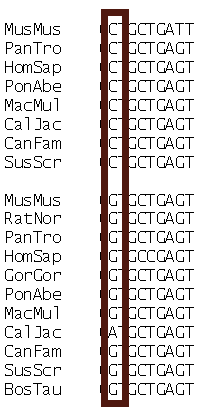
\includegraphics[width=0.2\textwidth]{figures/MCMC/TFBS.pdf}
%\captionbf{Sites utilis�s pour le MCMC}{

    %La position �tudi�e est celle encadr�e, contenant au total $10$ G, $8$ C et
    %$1$ A.

%}
%\label{fig:MCMC/TFBS}
%\efig

%\bfig
%\includegraphics[width=0.5\textwidth]{figures/MCMC/plotDirichlet.pdf}
%\captionbf{Distribution de la fonction de proposition $g(w_i^\text{inde} \to w)$}{

    %La distribution de Dirichlet est r�alis�e pour $50,000$ tirages al�atoires,
    %avec un bin de $0.02$. Les lignes verticales en pointill�s indiquent
    %l'estimation de la moyenne obtenue apr�s convergence (voir
    %fig.~\ref{fig:MCMC/plotConvergence}).

%}
%\label{fig:MCMC/plotDirichlet}
%\efig

\bfig
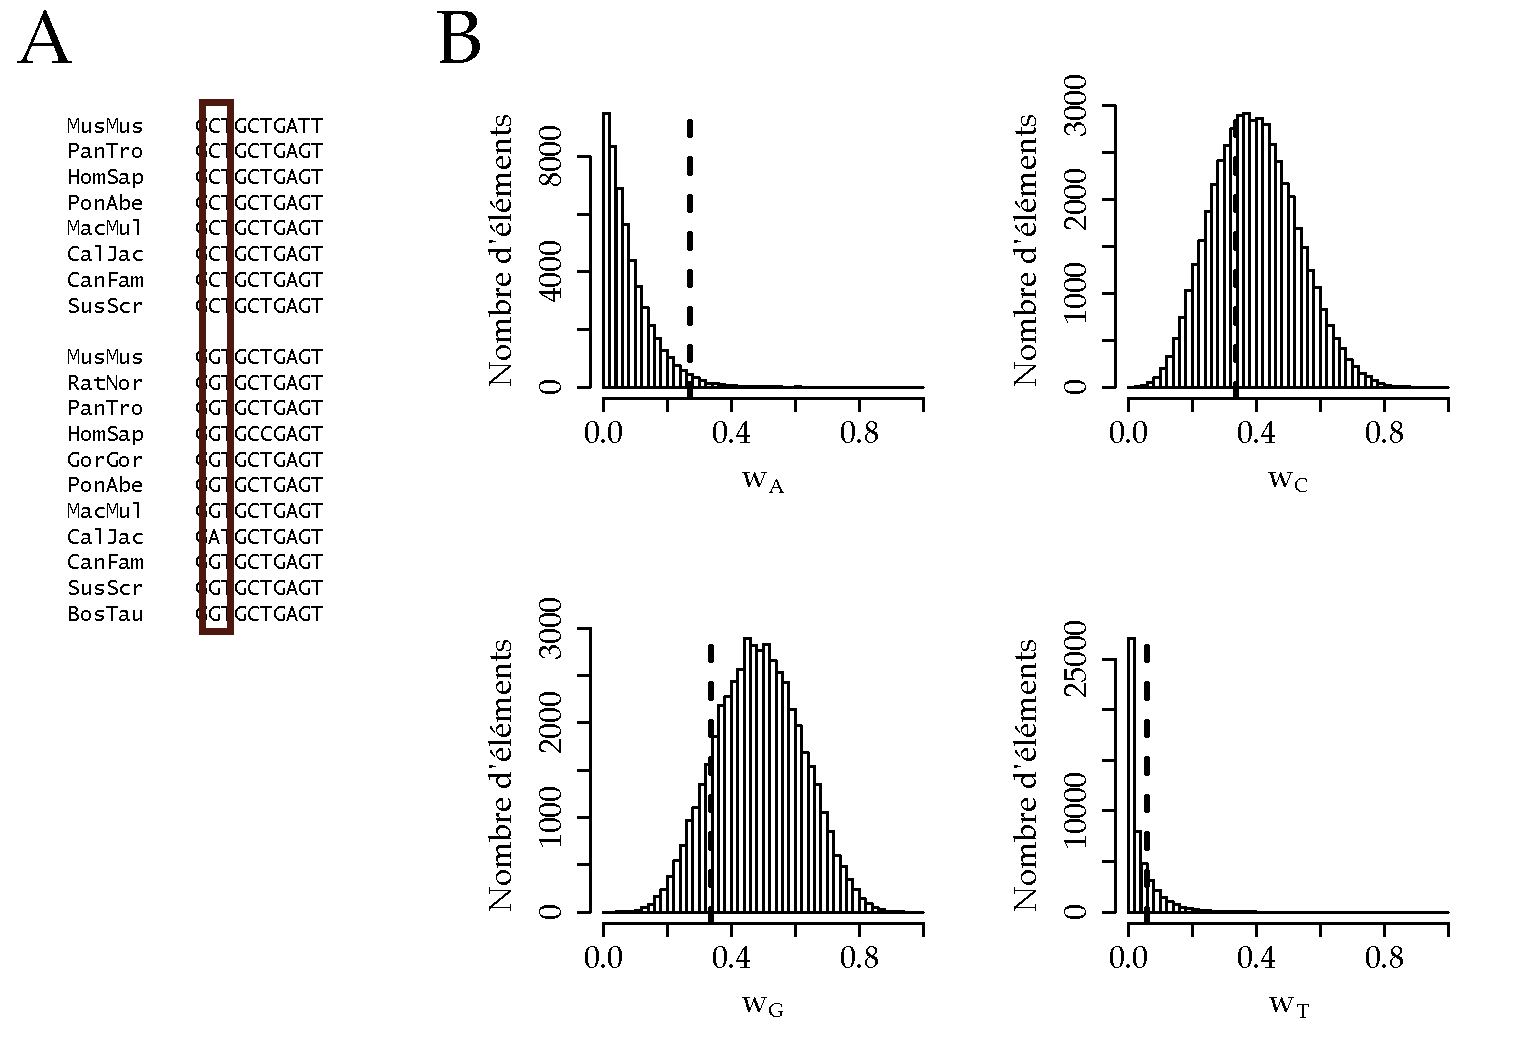
\includegraphics[width=1\textwidth]{figures/MCMC/sites-dirichlet.pdf}
\captionbf{Conditions initiales}{

    (A) Sites utilis�s pour le MCMC. On s'int�resse ici � la $2$�me position,
    contenant au total $10$ G, $8$ C et $1$ A.

    (B) Distribution de la distribution de Dirichlet correspondant � la
    proposition $g(w_i^\text{inde} \to w)$. L'�chantillonnage consiste en
    $50,000$ tirages al�atoires, et le bin est de $0.02$. Les lignes verticales
    en pointill�s indiquent l'estimation de la moyenne obtenue apr�s
    convergence (voir fig.~\ref{fig:MCMC/var_cv}).

}
\label{fig:MCMC/sites-dirichlet}
\efig

�tudions maintenant un exemple concret. Nous pr�sentons la m�thode sur le cas
pr�sent� en fig.~\ref{fig:MCMC/sites-dirichlet}A et nous utilisons le mod�le
d'�volution \textit{Felsenstein}. Le vecteur de poids $w_i$ est initialis� au
cas ind�pendant $w_i^\text{inde}$. La proposition $g(w_i^\text{inde} \to w)$
(�q.~\ref{eq:proposal})  est montr�e en fig.~\ref{fig:MCMC/sites-dirichlet}B.
On voit notamment comment la distribution de Dirichlet permet de rester dans le
simplexe dans les cas $w_A$ et $W_T$ proches de $0$. La valeur finale de
l'estimation de la moyenne de la post�rieure obtenue apr�s convergence de la
cha�ne (voir ci-dessous) est aussi montr�e : elle est relativement proche de la
moyenne de la distribution, indiquant que le choix de la valeur initiale est
effectivement judicieux.  \\


%\bfig
%\includegraphics[width=0.5\textwidth]{figures/MCMC/plotSampling.pdf}
%\captionbf{Extrait de l'�chantillonnage de $w_i$}{

%Les $500$ premiers �chantillons $w_i$ de la cha�ne MCMC sont montr�s.

%}
%\label{fig:MCMC/plotSampling}
%\efig

%\bfig
%\includegraphics[width=0.5\textwidth]{figures/MCMC/plotAutocorr.pdf}
%\captionbf{Fonction d'auto-corr�lation de la cha�ne MCMC}{

%Corr�lation entre des �chantillons s�par�s de $t-1$ it�rations. Une droite est
%ajust�e sur les $20$ premi�rs points, permettant de recueillir
%la pente $-T_b$ donnant le temps de d�corr�lation.

%}
%\label{fig:MCMC/plotAutocorr}
%\efig

\bfig
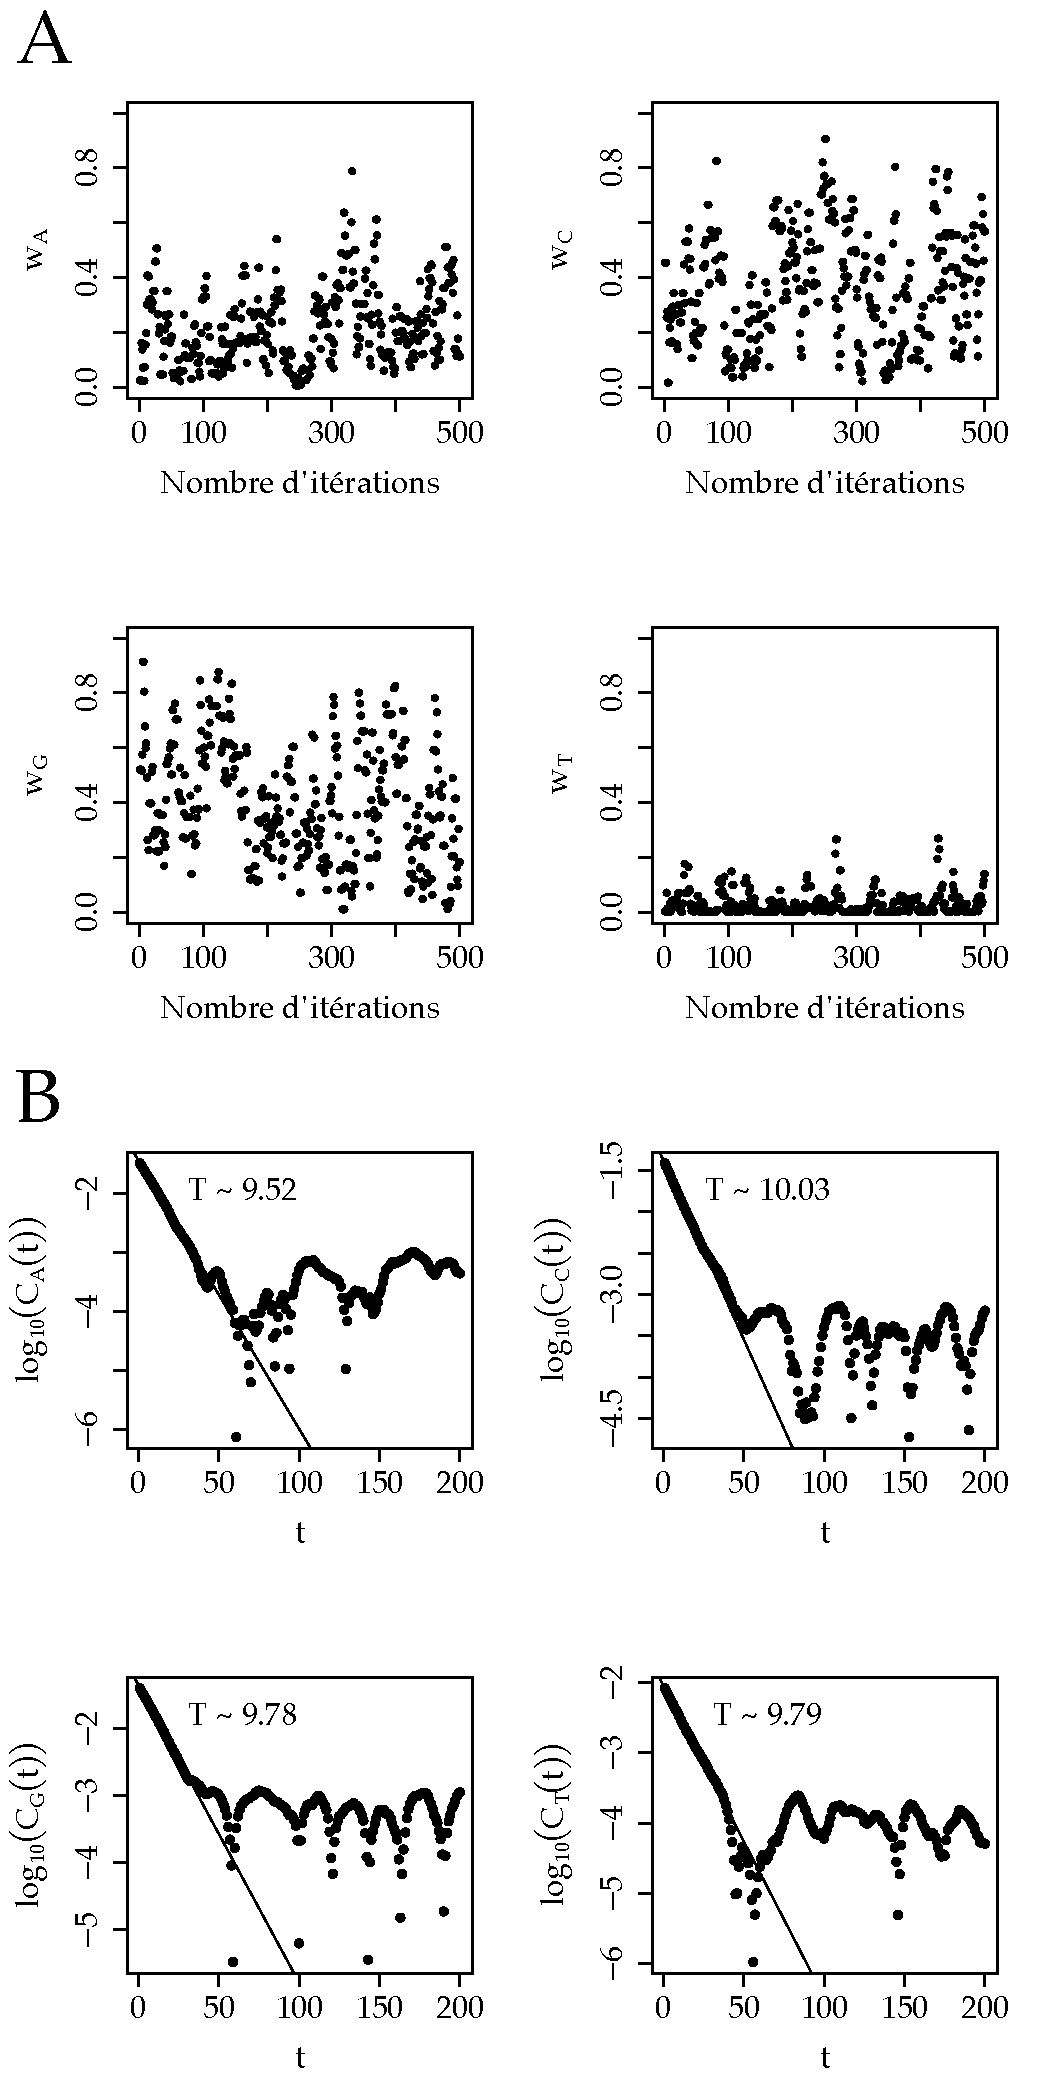
\includegraphics[width=0.6\textwidth]{figures/MCMC/sampling-autocorr.pdf}
\captionbf{Corr�lations entre les �chantillons}{

(A) Extrait de l'�chantillonnage de $w_i$. Les $500$ premiers �chantillons
$w_i$ de la cha�ne MCMC sont montr�s.

(B) Fonction d'auto-corr�lation de la cha�ne MCMC. La corr�lation $C_b(t)$ est
r�alis�e entre des �chantillons s�par�s de $t-1$ it�rations. Une droite est
ajust�e sur les $20$ premi�rs points, permettant d'obtenir la pente $-T_b$
donnant le temps de d�corr�lation.

}
\label{fig:MCMC/sampling-autocorr}
\efig

La cha�ne MCMC est ensuite lanc�e. Le taux d'acceptation est calcul� comme
valant $62\%$. Les $500$ premiers �chantillons de $w_i$ sont montr�s en figure
\ref{fig:MCMC/sampling-autocorr}A. On note que certains points semblent
corr�l�s : diminutions ou augmentations successives de la valeur courante
$w_i(t)$ sur plusieurs it�rations. Pour quantifier cet effet, nous avons mesur�
la corr�lation temporelle des �chantillons. Celle-ci est donn�e par

\begin{equation}
    C_b(\tau) = \frac{1}{N} \sum_{t=1}^{N-\tau} w_{i,b}(t) w_{i,b}(t+\tau) - \left(\frac{1}{N}\sum_{t=1}^N w_{i,b}(t)\right)^2
\end{equation}

avec dans ce cas $N=50,000$. Le logarithme de cette quantit� est montr�e en
figure \ref{fig:MCMC/sampling-autocorr}B. L'int�r�t du logarithme est de mettre
en exergue le caract�re exponentiel de la d�corr�lation
%\footnote{D'apr�s le
%th�or�me de Perron-Froebenius, le temps de d�correlation d'une cha�ne de Markov
%est donn� par $T=-1/\log(\mu)$, o� $\mu$ est la valeur propre de la cha�ne de
%Markov de plus grande valeur absolue} 
:

\begin{equation}
    C_b(\tau) \propto e^{-\tau/T_b}
\end{equation}

Les temps de d�correlation $T_b \sim 10$ sont estim�s en ajustant une droite
sur les $20$ premiers points de la courbe. Maintenant que l'on connait le temps
de corr�lation entre deux �chantillons, il est possible d'obtenir des
�chantillons ind�pendants en les choisissant � des intervalles grands devant
$T_b$. Dans notre cas, nous avons choisis un intervalle de $30$ it�rations.  \\

\bfig
%\includegraphics[width=0.5\textwidth]{figures/MCMC/plotCVvar.pdf}
%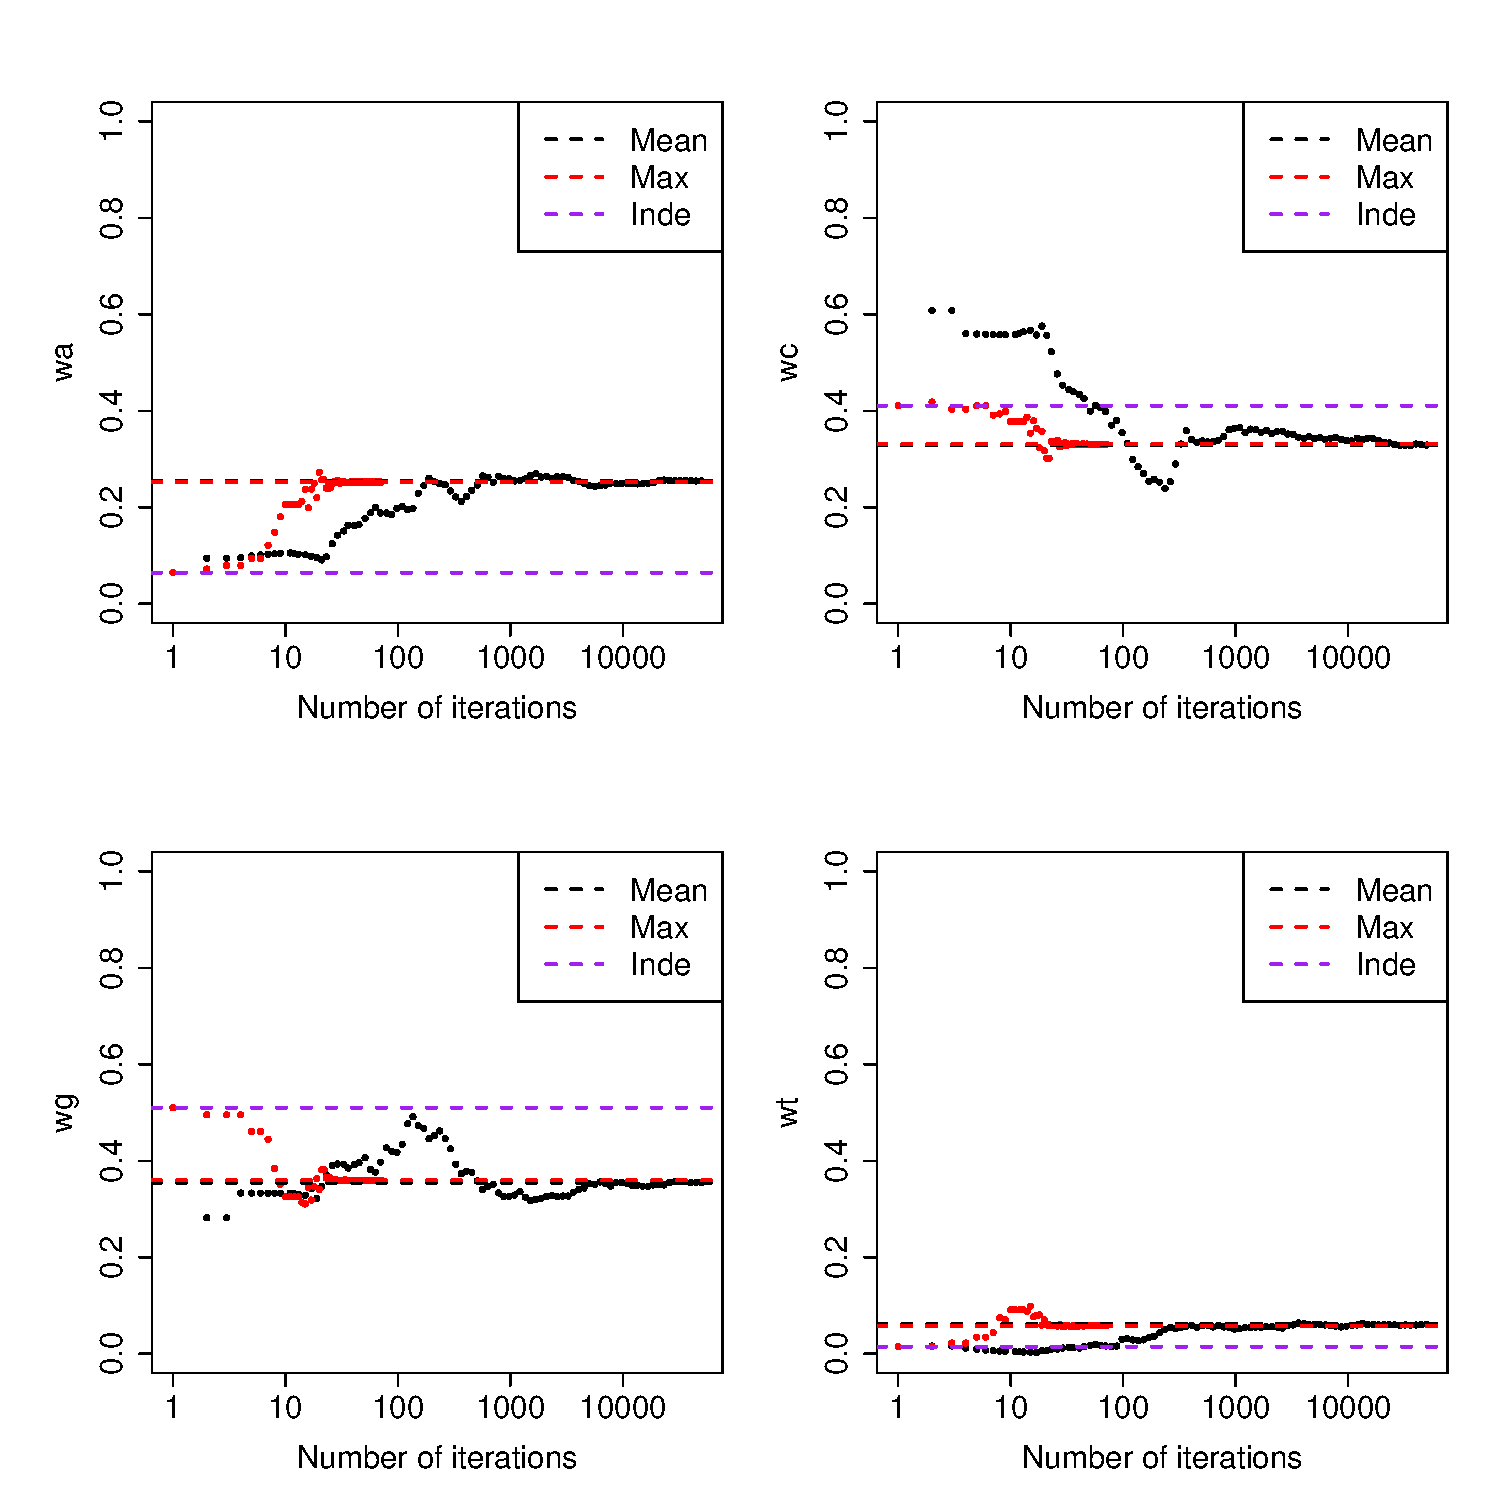
\includegraphics[width=0.5\textwidth]{figures/MCMC/plotConvergence.pdf}
\includegraphics[width=0.55\textwidth]{figures/MCMC/var-cv.pdf}
\captionbf{Estimation de la convergence}{

   
    
    (A) �cart-type $\sigma_b$ de la distribution $w_{i,b}$ estim� � partir de
    $n$ �chantillons ind�pendants. Ces �chantillons sont pris toutes les $30$
    it�rations au sein de la cha�ne MCMC, soit environ $3$ fois le temps de
    d�corr�lation. On observe qu'au bout de $100$ it�rations l'�cart-type est
    stabilis�. Par ailleurs les fluctuations sont relativement faibles, au plus
    de l'ordre de $\sim 10\%$ de la moyenne.

    (B) La convergence est estim�e gr�ce au Th�or�me Centrale Limite.
    L'�cart-type de l'estimateur de la moyenne se comporte comme  $\sigma_b
    / \sqrt{n}$. La pr�cision demand�e correspond � un �cart-type $\leq 5\%$ de
    la moyenne pour les $4$ bases, ce qui correspond � l'intersection la plus
    tardive entre les courbes noires et grises (dans notre cas le cadran du bas
    � droite).

}
\label{fig:MCMC/var_cv}
\efig

Nous souhaitons maintenant �tudier la convergence de la cha�ne MCMC. Pour cela,
nous utilisons le Th�or�me Central Limite (TCL, cf
\ref{sub:principe_de_l_algorithme_de_metropolis_hastings}).  Celui-ci stipule
que pour un  nombre $n$ suffisamment grand d'�chantillons ind�pendants,
l'�cart-type de la distribution de l'estimateur empirique de la moyenne
$\hat{w}_n$ se comporte comme $\sigma_b / \sqrt{n}$, o� $\sigma_b$ est
l'�cart-type de la distribution $\mathcal{P}(w_i|\mathcal{A})$. Ce dernier doit
lui-m�me �tre estim� � partir de la cha�ne MCMC. Nous pr�sentons en figure
\ref{fig:MCMC/var_cv}A la valeur de l'estimation $\sigma_b(n)$ obtenue pour $n$
it�rations ind�pendantes. On voit que cette valeur atteint rapidement en
$\sim100$ it�rations une valeur stable, et que dans tous les cas les
fluctuations sont faibles, de l'ordre de $10\%$ de $\hat{w}_n$. Il para�t donc
raisonnable d'utiliser cette valeur de $\sigma_b$ pour le TCL. Nous tra�ons en
figure \ref{fig:MCMC/var_cv}B la quantit� $\sigma_b(n)/\sqrt{n}$. La cha�ne est
consid�r�e comme converg�e lorsque cette valeur est inf�rieure ou �gale � $5\%$
de la valeur moyenne estim�e $\hat{w}_n$ (ligne grise) dans les $4$ cas.
Ce seuil est bien entendu arbitraire et d�pend de la pr�cision voulue par
l'utilisateur sur l'estimation. N�anmoins, une plus grande pr�cision implique
un plus long temps de calcul.  \\

Nous comparons finalement en figure \ref{fig:MCMC/plotConvergenceCompare} la
valeur de l'estimation du Maximum A Posteriori (MAP) de la post�rieure modifi�e
(voir article) obtenue avec la m�thode de descente de gradient et celle de la
moyenne de la post�rieure obtenue avec l'approche MCMC, en fonction du nombre
d'it�rations (toutes les it�rations, pas seulement les �chantillons
ind�pendants).  L'approche MCMC, bien que convergeant vers un �tat proche de
celui donn� par la descente de gradient, met beaucoup plus de temps � converger
: plus de $10,000$ it�rations, alors que la descente de gradient n'en requiert
que $100$. Au vu de la faible diff�rence entre les deux r�sultats, nous
utilisons dans Imogene l'approche de maximisation de la post�rieure modifi�e,
ce qui permet un gain de temps consid�rable pour l'algorithme (au minimum un
facteur $10$).


\bfig
\includegraphics[width=1\textwidth]{figures/MCMC/plotConvergenceCompare.pdf}
\captionbf{Comparaison des approches par MCMC et par descente de gradient}{

L'approche de maximisation de (l'oppos� de) la post�rieure modifi�e par
descente de gradient (rouge, cf article) est compar�e � l'approche de calcul de
la moyenne de la post�rieure par MCMC (noir). Les deux m�thodes sont
initialis�es au m�me $w_i^{\text{inde}}$. Alors que la descente de gradient
converge rapidement ($\sim100$ it�rations), l'approche MCMC converge plus
lentement, dans ce cas plus de $10,000$ it�rations. Au final les deux approches
convergent vers des quantit�s proches (lignes pointill�es rouges et noires). 

}
\label{fig:MCMC/plotConvergenceCompare}
\efig

% subsection illustration_de_la_m_thode_mcmc_sur_un_exemple (end)


% section calcul_de_la_moyenne_de_la_post_rieure_par_une_m_thode_mcmc (end)

\newpage

%%%%%%%%%%%%%%%%%%%%%%%%%%%%%%%%%%%%%%%%%%%%%%%%%%%%%%%%%%%%%%%%%%%%%%%%%%%%%%%%%%%%%%%%%%%
\chapter{\ChTrichomes}
\ifthenelse{\FaitMinitocs > 0}{\adjustmtc \minitoc}{Minitoc}
\newpage
\section*{Introduction du chapitre \thechapter}

%\includepdf[pages=-]{articles/trichomes-plosbiol-merged.pdf}

%%%%%%%%%%%%%%%%%%%%%%%%%%%%%%%%%%%%%%%%%%%%%%%%%%%%%%%%%%%%%%%%%%%%%%%%%%%%%%%%%%%%%%%%%%%%%%%%%%%	%%%%%%%%%%%%%%%%%%%%%%%%%%%%%%%%%%%%%%%%%%%%%%%%%%%%%%%%%%%%%%%%%%%%%%%%%%%%%%%%%%%%%%%%%%%%%%%%%%%	
\newpage
\section{}

			
%%%%%%%%%%%%%%%%%%%%%%%%%%%%%%%%%%%%%%%%%%%%%%%%%%%%%%%%%%%%%%%%%%%%%%%%%%%%%%%%%%%%%%%%%%%%%%%%%%%	%%%%%%%%%%%%%%%%%%%%%%%%%%%%%%%%%%%%%%%%%%%%%%%%%%%%%%%%%%%%%%%%%%%%%%%%%%%%%%%%%%%%%%%%%%%%%%%%%%%	
\newpage	
			
\section*{Conclusion du chapitre \thechapter}

%\includepdf[pages=-]{articles/trichomes-plosbiol-merged.pdf}
\newpage
%%%%%%%%%%%%%%%%%%%%%%%%%%%%%%%%%%%%%%%%%%%%%%%%%%%%%%%%%%%%%%%%%%%%%%%%%%%%%%%%%%%%%%%%%%%
%\chapter{\ChMuscle}
%\label{chap:muscle}
%\ifthenelse{\FaitMinitocs > 0}{\adjustmtc \minitoc}{Minitoc}
%\newpage
%\section*{Introduction du chapitre \thechapter}

Cette derni�re partie est consacr�e � l'�tude de la diff�renciation musculaire.
Ce travail a �t� effectu� en collaboration avec l'�quipe de Pascal Maire
� l'Institut Cochin, qui m'a accueilli et m'a permis de r�aliser une partie des
exp�riences pr�sent�es, avec l'aide de Iori Sakakibara. Nous nous int�ressons
ici particuli�rement aux hom�oprot�ines Six$1$ et Six$4$ (r�f�r�es dans la
suite par \sixd) qui sont des \tfs impliqu�s dans la r�gulation des stades
successifs de la myogen�se. Ils activent en effet les TFs n�cessaires
� l'engagement de cellules pluripotentes dans la voie myog�nique et � leur
diff�rentiation : Pax3 ainsi que les Facteurs de R�gulation Myog�nique Myf5,
Mrf4, Myod et Myog. Cette r�gulation passe par la fixation des prot�ines Six
sur un site \mef d'environ $10$bp. 

Nous nous sommes d'abord int�ress� aux cibles transcriptionnelles de \sixd
� l'�chelle du g�nome, ainsi qu'� leurs cor�gulateurs. Pour cela, nous avons
d'abord r�alis� un mod�le PWM des sites \mef, que nous avons utilis� pour la
pr�diction de sites. Nous avons par ailleurs r�cup�r� de nombreuses donn�es
relatives � la diff�renciation musculaire : \chipseq de TFs et des marques
�pig�n�tiques des histones, donn�es d'expression de type RNAseq, sites de
fixation conserv�s que nous avons obtenus par analyse bioinformatique, etc. Ces
donn�es ont �t� regroup�es sur le visualiseur de UCSC, permettant d'envisager
facilement le contexte de r�gulation de certains g�nes d'int�r�t. Nous
pr�sentons plusieurs validations de pr�dictions obtenues par analyse
bioinformatique avec ces donn�es.

Par ailleurs, nous nous sommes int�ress� � l'action concert�e ou
\textit{synergie} entre \sixd et le TF ma�tre MyoD au cours de la
diff�renciation musculaire. Nous avons trouv� un certain nombre de CRMs fix�s
par MyoD et poss�dant un site \mef conserv� chez les mammif�res, et dont le
g�ne le plus proche n'est activ� qu'en pr�sence de MyoD et de \sixd. Parmi les
g�nes en question figurent \myog, TF requis pour la diff�renciation terminale,
et des g�nes structuraux comme \textit{Tnnc1} ou \textit{Ttn}. Nous avons test�
l'activit� des CRMs pr�dits et en avons trouv� $72\%$ qui r�capitulent
l'expression du g�ne le plus proche lorsqu'ils sont test�s par transfection
avec un rapporteur Lucif�rase. Nous avons par ailleurs utilis� Imogene pour
pr�dire des cor�gulateurs et avons test� l'importance des sites par mutagen�se.

%%%%%%%%%%%%%%%%%%%%%%%%%%%%%%%%%%%%%%%%%%%%%%%%%%%%%%%%%%%%%%%%%%%%%%%%%%%%%%%%%%%%%%%%%%%%%%%%%%%	%%%%%%%%%%%%%%%%%%%%%%%%%%%%%%%%%%%%%%%%%%%%%%%%%%%%%%%%%%%%%%%%%%%%%%%%%%%%%%%%%%%%%%%%%%%%%%%%%%%	
\newpage

\section{Introduction � la myogen�se squelettique} 
\label{sec:introduction_la_myogen_se}

\subsection{Les diff�rentes �tapes de la myogen�se}
\label{sub:les_diff_rentes_tapes}

La myogen�se correspond � la formation des tissus musculaires, ceux-ci �tant
regroup�s en trois types majeurs : les muscles cardiaques, les muscle lisses et
les muscles squelettiques. C'est la formation de ces derniers qui nous
int�resse ici. Les muscles squelettiques sont compos�s de fibres musculaires polynucl�es
provenant de la fusion de prog�niteurs musculaires appel�s myoblastes. Ils sont
sous le contr�le du syst�me nerveux central, et composent l'un des organe
majeur des vert�br�s, concentrant $\sim40\%$  du poids corporel. La
myogen�se squelettique d�bute relativement t�t au cours de l'embryogen�se : � $8.5$
jours\footnote{La mi-journ�e correspondant au fait que la f�condation a lieu la
nuit.} apr�s f�condation (ou E$8.5$ pour \textit{Embryonic day} $8.5$) chez
l'embryon de souris sur un total de $18$ jours embryonnaires. Elle a lieu au
niveau des somites, structures p�riodiques situ�es au niveau des futures
vert�bres (fig.~\ref{fig:buckingham-myogenesis}a). Les �tapes de fusion des
myoblastes et de maturation des fibres s'�talent ensuite sur toute
l'embryogen�se (fig.~\ref{fig:buckingham-myogenesis}b), ainsi que dans le
muscle adulte lors de la r�g�n�ration musculaire \cite{Parker2003p761}.

\bfigp
\includegraphics[width=.9\textwidth]{figures/buckingham-myogenesis.pdf}
\captionbf{Formation du muscle squelettique chez l'embryon de souris}{

    Figure tir�e de \citet{Buckingham2007p776} illustrant les diff�rentes
    �tapes de la myogen�se. (a) Le dermomyotome �pith�lial d'un somite (vert)
    ainsi que le muscle squelettique du myotome (beige) sont d'abord form�s par
    la d�lamination des cellules provenant des extr�mit�s du dermomyotome
    (fl�ches bleues) : c'est la premi�re vague de la myogen�se. Ensuite, lors
    d'une deuxi�me vague, le dermomyotome central perd sa structure �pith�liale
    et des cellules musculaires prog�nitrices s'int�grent au myotome
    (fl�ches rouges). Les TFs pr�curseurs de ces �v�nements sont indiqu�s en
    rouge. (b) Sch�ma montrant les �tapes de diff�renciation des prog�niteurs
    musculaires, ainsi que les temps de d�veloppement associ�s (E : jour
    embryonnaire).

}
\label{fig:buckingham-myogenesis}
\efigp


% subsection les_diff_rentes_tapes (end)

\subsection{Les Facteurs de R�gulation Myog�nique et leurs cofacteurs}
\label{sub:la_r_gulation_g_n_tique_les_facteurs_de_r_gulation_myog_nique_ou_mrfs}

D'un point de vue g�n�tique, la myogen�se des vert�br�s est coordonn�e en
partie par l'action de $4$ Facteurs de R�gulation Myog�nique (MRF pour
\textit{Myogenic Regulatory Factors}) : MyoD, Myf5, Mrf4 et Myog, qui font
partie de la famille de prot�ines \textit{basic Helix-Loop-Helix} (bHLH) et se
fixent sur les bo�tes E (ou E-box) du type CANNTG.  Ces MRFs sont activ�s
successivement � travers une cascade de r�gulation g�n�tique, et se r�gulent les
uns les autres. Par exemple, Myf5, MRF4 et MyoD peuvent activer MyoD ; Myf5,
MyoD et Mrf4 r�gulent l'expression de Myog ; et Myog peut activer l'expression
de Mrf4 \cite{Naidu1995uq}. En outre, MyoD et Myog peuvent s'auto-activer
\cite{Thayer1989kx}. Enfin, un certain degr� de redondance a �t� observ� entre
Myf5, Mrf4 et MyoD au cours du d�veloppement embryonnaire de la souris, et
l'analyse des embryons KO pour ces g�nes a conduit � la conclusion qu'ils ont
tous la capacit� d'activer la myogen�se � partir de cellules embryonnaires
pluripotentes et d'agir comme des g�nes de d�termination
\cite{KassarDuchossoy2004p823}. 


Ces MRFs sont la cl� de vo�te de la diff�renciation myog�nique. Cependant, la
r�gulation pr�cise du r�seau de g�nes activ�s par les MRFs n�cessite leur
coop�ration avec d'autres facteurs de transcription. En particulier, la liaison
de MyoD � l'ADN n'est pas pr�dictive d'une activit� enhancer
\cite{Cao2010p1805}. Ainsi, \citet{Molkentin1996p646} ont montr� que
l'activation transcriptionnelle par les MRFs est renforc�e par la fonction des
TFs � bo�te MADS MEF$2$. Leur importance a ult�rieurement �t� confirm�e par les
travaux de \citet{Blais2005p809} : en utilisant un grand nombre de g�nes cibles
des MRFs, les auteurs ont cherch� dans leur r�gion promotrice des sites de
liaison sur-repr�sent�s pour les TFs issus de la base de donn�es Transfac. Ils
ont ainsi constat� que l'�l�ment riche en A/T reconnu par MEF2 �tait parmi eux,
et ont confirm� son recrutement � plusieurs de ces sites.  Par ailleurs, un
autre motif d'ADN trouv� comme sp�cifiquement enrichi parmi les promoteurs
cibles des MRFs �tait l'�l�ment \mef (consensus GAAACCTGA), le site de liaison
des hom�oprot�ines Six. Cette s�quence \mef �tait particuli�rement abondante au
sein des promoteurs des g�nes dont l'expression �tait induite de mani�re
significative au cours de la diff�renciation.
% subsection
% la_r_gulation_g_n_tique_les_facteurs_de_r_gulation_myog_nique_ou_mrfs (end)



\subsection{Les hom�oprot�ines Six}
\label{sub:les_hom_oprot_ines_six}

Les hom�oprot�ines Six associ�es aux sites MEF$3$ poss�dent un r�le �tendu au
cours de la myogen�se, et nous en pr�sentons maintenant les d�tails.  Parmi les
6 g�nes appartenant � la famille des hom�oprot�ines Six
  (fig.~\ref{fig:kawakami-six-expression}), \textit{Six$1$} et \textit{Six$4$}
  ont re�u une attention particuli�re dans le contexte de la myogen�se
  squelettique, bien que d'autres membres comme \textit{Six$2$} ou
  \textit{Six$5$} semblent �tre en mesure de compenser partiellement leur perte
  \cite{Relaix2013ve}. Ces deux g�nes se trouvent � proximit� l'un de l'autre
  sur le chromosome $12$ de la souris et sont s�par�s par $100$kb de s�quence
  interg�nique. L'�quipe de Pascal Maire a d�j� identifi� plusieurs fonctions
  cl�s de \textit{Six$1$} dans le lignage musculaire au cours de
  l'embryogen�se, par l'analyse de mod�les de souris d�pourvues de
  \textit{Six$1$} (Six$1$KO) et de Six$1$ et Six$4$ (\sixdko), et par des
  exp�riences de \chip.  L'analyse des embryons \sixdko \cite{Grifone2005vn}
  � E$10$ \cite{Niro2010p3444} et E$18$ \cite{Richard2011ys} a permis
  d'identifier des cibles g�n�tiques directes et indirectes de Six$1,4$, et
  a d�voil� plusieurs fonctions des hom�oprot�ines Six pendant le d�veloppement
  musculaire et la sp�cialisation des fibres musculaires.  

\bfig
\includegraphics[width=1\textwidth]{figures/kawakami-six-expression.pdf}
\captionbf{Motifs d'expression et localisation g�nomique des g�nes de la famille Six}{

    Figure tir�e de \cite{Kawakami2000bh}, montrant les motifs d'expression des
    g�nes de la famille Six chez l'embryon (A) et dans l'oeil (B) � E$13.5$.
    Les couleurs similaires refl�tent des motifs d'expression similaires. La
    localisation chromosomique des g�nes est aussi montr�e en (C). 

}
\label{fig:kawakami-six-expression}
\efig


Les principaux points sont les suivants (fig.~\ref{fig:muscle/myogenese_six})
: Six$1$ et Six$4$ sont requis pour la gen�se des prog�niteurs myog�niques
hypaxiaux (\cad ventraux).  En l'absence de Six$1$ et Six$4$, les cellules
ventrales pluripotentes du dermomyotome somitique ne parviennent pas � adopter
un destin de prog�niteur myog�nique et elles n'expriment ni \textit{Pax3} ni
les MRFs. Six$1$ et Six$4$ contr�lent directement l'expression de
\textit{Pax$3$} \cite{Grifone2007p728}, et donc l'engagement des cellules
pluripotentes dermomyotomales dans un destin de prog�niteur myog�nique.  Plus
tardivement, l'expression de \textit{Myf$5$} dans le membre est contr�l�e par
un enhancer \og membre \fg li� par les prot�ines Six$1$ et Six$4$, et cette
liaison est n�cessaire pour permettre l'expression de Myf$5$
\cite{Giordani2007p473}. Par ailleurs, deux enhancers contr�lent sp�cifiquement
l'expression de MyoD au cours de l'embryogen�se et au cours de la r�g�n�ration
du muscle adulte: le \textit{Distal Regulatory Region} ou DRR
\cite{Asakura1995ly} et le \textit{Core Enhancer} ou CE
\cite{Kucharczuk1999zr}. La liaison de ces �l�ments par Six$1$ et Six$4$ a �t�
confirm�e par \chip au cours de l'embryogen�se (\citet{Relaix2013ve}, voir
section \ref{sub:r_gulation_de_myod1_par_les_prot_ines_six}) ainsi que dans des
cultures de cellules satellites \cite{Le-Grand2012qf}, qui sont des cellules
souches du muscle adulte activ�es lors de la r�g�n�ration musculaire.
L'expression de Mrf$4$ n'est pas d�tect�e chez les embryons \sixdko � E$10$
\cite{Grifone2007p728}. Myog est aussi sous le contr�le direct des prot�ines
Six \cite{Spitz1998p3285}. Enfin, les prot�ines Six r�gulent des g�nes
sp�cifiques des fibres glycolytiques de type rapide (voir section
\ref{sub:r_gulation_d_un_lincrna_par_six_dans_le_muscle_adulte}). Par exemple,
la mutation du site MEF$3$ au sein du promoteur de \textit{Aldoa}, g�ne codant
pour une enzyme impliqu�e dans la glycolyse, entra�ne l'abolition de
l'expression d'un transg�ne rapporteur dans des myofibres adultes
\cite{Spitz1997p455}.

\bfig
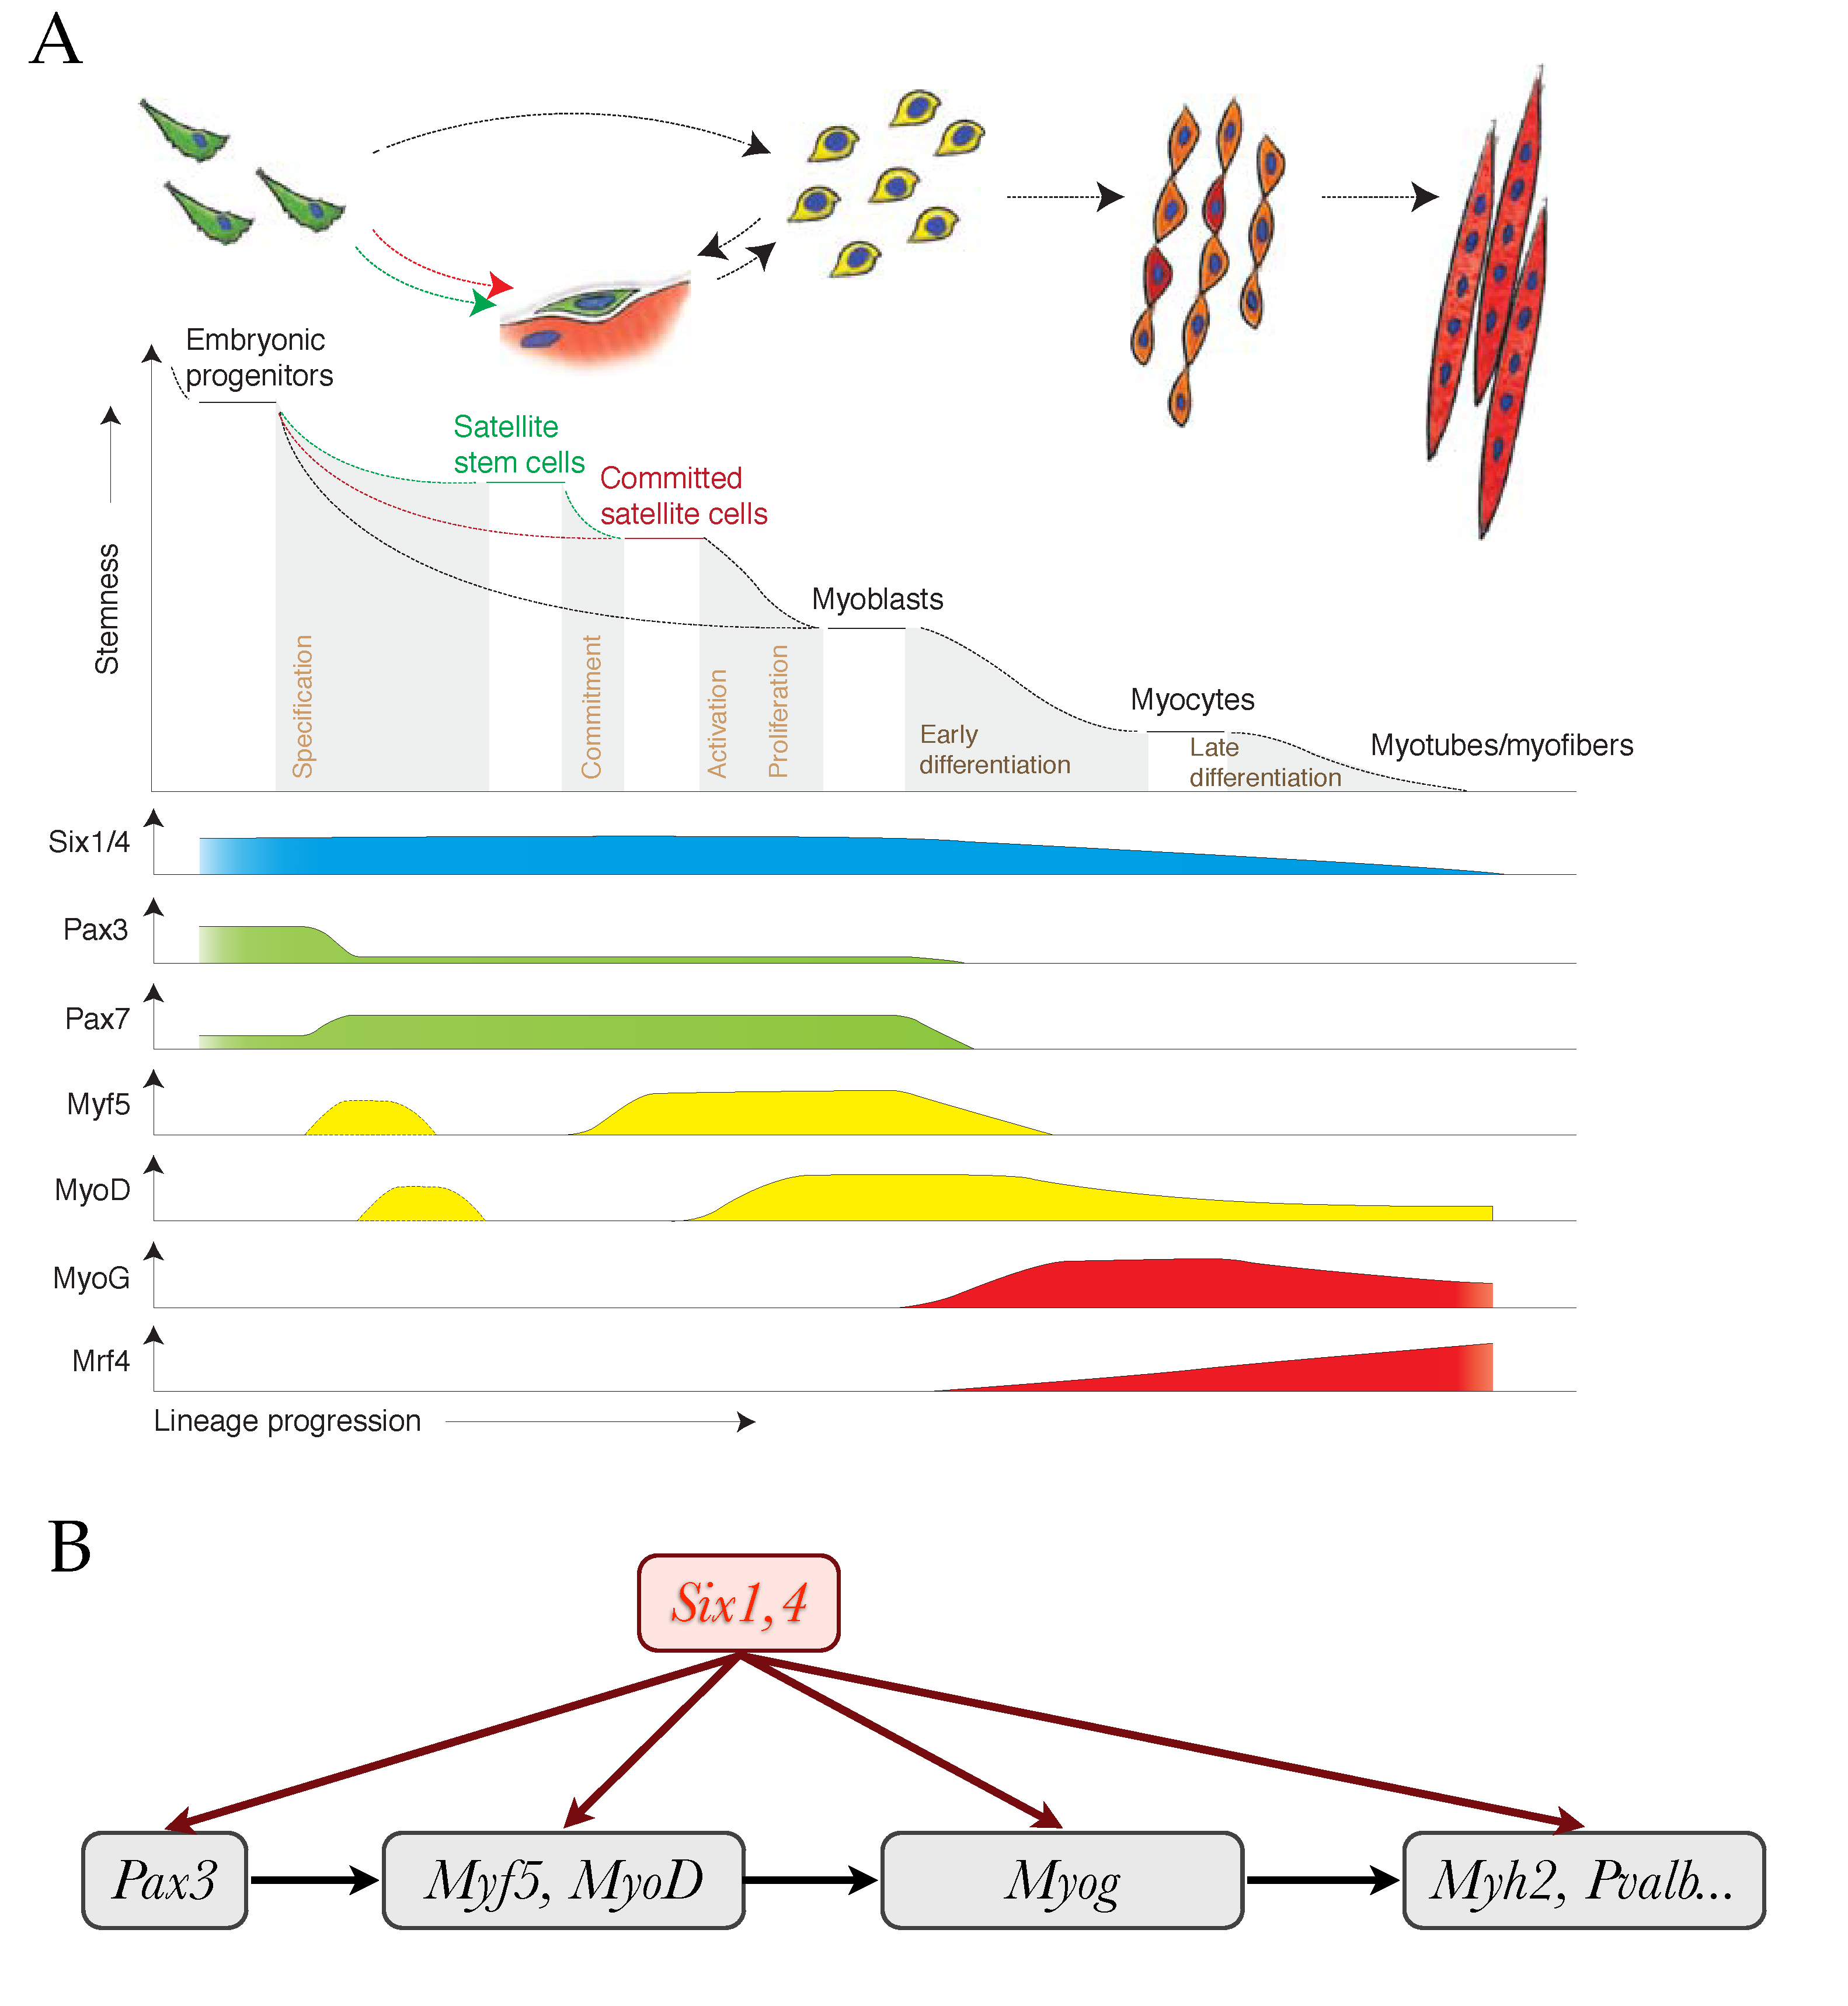
\includegraphics[width=1\textwidth]{figures/muscle/myogenese_six.pdf}
\captionbf{R�le des prot�ines Six au cours de la myogen�se}{

La myogen�se embryonnaire consiste en plusieurs �tapes de diff�renciation
musculaire : la gen�se des prog�niteurs myog�niques ou myoblastes, exprimant
\textit{Pax3}, l'induction des g�nes de d�termination myog�nique comme
\textit{Myf5} et \textit{Myod1}, la diff�renciation des myoblastes et leur
fusion en myotubes avec l'expression de \textit{Myog}. Les myotubes se
sp�cialisent plus tardivement en fibres de type lentes (oxydatives) ou rapides
(glycolytiques). Les hom�oprot�ines Six interviennent dans la r�gulation de ces
diff�rentes �tapes en r�gulant les TFs indiqu�s. Des cor�gulateurs peuvent
intervenir dans la r�gulation (disque jaune).

}
\label{fig:muscle/myogenese_six}
\efig

%Ainsi, Six$1$ et Six$4$ contr�lent directement Pax$3$ et tous les MRF, mais ce
%contr�le est spatialement (axe dorso-ventral et axe ant�ro-post�rieur)
%h�t�rog�ne dans l'embryon.




%Par analyse
%bioinformatique, j'ai trouv� deux MEF3 sites dans le noyau activateur et un
%MEF3 site du RRC.  Mutation de ces trois MEF3 des sites aboli par plus de 95%
%l'expression d'un journaliste du transg�ne MyoD dans une souris transg�nique
%essai transitoire � E11.5 dans toutes les lign�es myog�niques (tronc, membres,
%t�te) (Relaix
%2012). 


%Mutations introduites dans le site MEF3 pr�sente dans le
%promoteur myog�nine abolies expression d'une �-galactosidase transg�ne
%rapporteur myog�nine cours de l'embryogen�se (Spitz,1998), et les mutations
%introduites dans le site MEF3 pr�sente dans le promoteur AldolaseA abolis
%l'expression d'un transg�ne rapporteur dans myofibres adultes (Spitz, 1997).
%Par cons�quent, six prot�ines apparaissent comme de bons candidats pour MFR de
%modulation de la r�gulation transcriptionnelle.  N�anmoins, la coop�ration des
%centres de tri et TFS associ�s est loin d'�tre enti�rement comprise, et la
%coop�ration des centres de tri avec non pas un, mais une vari�t� de facteurs de
%transcription, par exemple � diff�rents moments au cours de l'embryogen�se,
%afficher une croissance musculaire natale et pendant la r�g�n�ration du muscle
%adulte est susceptible de se produire sur diff�rents activateurs de g�nes
%cibles.



% subsection les_hom_oprot_ines_six (end)



\FloatBarrier
% section introduction_la_myogen_se (end)

\section{Int�gration de donn�es bioinformatiques et exp�rimentales sur le muscle} 
\label{sec:integration_de_donn_es_bioinformatiques_et_exp_rimentales_sur_le_muscle}

La premi�re �tape de notre collaboration avec l'�quipe de P. Maire a �t� de
construire un mod�le de motif pour les sites de fixation \mef associ�s aux
prot�ines \sixd chez la souris. Un tel motif, qui n'existait jusqu'alors pas,
permet de r�aliser des pr�dictions pr�cises, et nous discuterons apr�s de leur
v�rification.  Par ailleurs, nous avons r�cup�r� de nombreuses donn�es
exp�rimentales dans la litt�rature sur la diff�renciation musculaire (\chipseq,
RNAseq, donn�es �pig�n�tiques\ldots) et les avons int�gr�es au syst�me de
visualisation de UCSC (pr�sent� en introduction, section
\ref{sub:outils_visualisation}).  L'int�gration de ces multiples donn�es permet
d'appr�hender facilement et rapidement les ph�nom�nes de r�gulation ayant lieu
lors de la diff�renciation musculaire � l'�chelle locale de g�nes d'int�r�t
comme � l'�chelle globale g�nomique en croisant les donn�es. 


\subsection{Obtention d'une PWM optimale pour MEF3}
\label{sub:obtention_d_une_pwm_optimale_pour_mef3}

\begin{table}[!t]
\centering
%\resizebox{8cm}{!} {
\begin{tabular}{|l|l|}
\hline
myog-spitz-pascal & \texttt{GAAACCTGA} \\
pax3-pascal & \texttt{GAAATCTAA} \\
myf5-pascal & \texttt{GTAACTGGA} \\
myod-DRR-lhonore-pascal & \texttt{GAAACCGGA} \\
Mlc-hox-pascal & \texttt{GTAATTTAA} \\
atp2a1-1-niro-pascal & \texttt{GTAACTGGA} \\
atp2a1-2-niro & \texttt{GTAACCTGA} \\
tnnc2-niro & \texttt{GAAATTTAA} \\
Nrk-pascal & \texttt{GCAAGGCGA} \\
sarcalumenin-pascal & \texttt{GGAACTTGA} \\
myl1-2-niro & \texttt{GAAATTGAA} \\
ifitm3-niro & \texttt{GTAATTTGA} \\
mybph-2-niro & \texttt{GAAATCTGA} \\
myeov2-niro & \texttt{GAAACTTGA} \\
\hline
\end{tabular}
\begin{tabular}{|l|l|}
\hline
aldo-spitz-pascal & \texttt{GAAACCTGA} \\
ato-pascal & \texttt{GTCATTTGA} \\
kcne1l-niro & \texttt{GATAACGGA} \\
myf5-personal-josiane & \texttt{GAAATTTAA} \\
pax3-1-personal-josiane & \texttt{GAAATGTAA} \\
pax3-2-personal-josiane & \texttt{GTTACTGGA} \\
pvalb-personal-iori & \texttt{GTAACCTGA} \\
Utrophine-pascal & \texttt{GTCACCTGA} \\
Na-K-ATPase-pascal & \texttt{GCAACCTGA} \\
myf5-2-pascal & \texttt{GCAACCTGA} \\
myf5-sat-pascal & \texttt{GAAATCTGA} \\
lbx1-pascal & \texttt{GCCACCTGA} \\
MCK-pascal & \texttt{GACACCCGA} \\
IgfBp5-pascal & \texttt{GCAATTTGA} \\
troponine-C-low-pascal & \texttt{GTAACCTGA} \\
sarcalumenin-pascal & \texttt{GGAACTTGA} \\
Nrk-pascal & \texttt{GCAAGGCGA} \\
Tp4-pascal & \texttt{GCAAGCAGA} \\
\hline
\end{tabular}
%}
\captionbf{Sites \mef positifs}{ 
    
    Le tableau de gauche correspond aux $14$ sites conserv�s chez les
    mammif�res que nous avons utilis�s pour l'apprentissage de la PWM \mef, et
    le tableau de droite aux sites utilis�s comme un ensemble test ind�pendant
    de Vrais Positifs dans la courbe ROC de la figure
    \ref{fig:muscle/roc-mef3}.

}
\label{tab:mef3_pos}
\end{table}

\begin{table}[!t]
\centering
%\resizebox{8cm}{!} {
\begin{tabular}{|l|l|}
\hline
myf5-1-personal & \texttt{GACAGTGGA} \\
myf5-2-personal & \texttt{GTAACCTCA} \\
myf5-mut & \texttt{GTAACTGGG} \\
pax3-1-pascal & \texttt{GGAACTTGA} \\
pax3-2-pascal & \texttt{GTATTAATA} \\
pax3-3-pascal & \texttt{GGATAAAGA} \\
pax3-4-pascal & \texttt{GCTAATTGA} \\
pax3-5-pascal & \texttt{GAAAGATTA} \\
pax3-6-pascal & \texttt{GCTCTCTGA} \\
pax3-7-pascal & \texttt{GAGCCCTGA} \\
pvalb-1-personal & \texttt{GCACAATGA} \\
pvalb-2-personal & \texttt{GCAGGCTGA} \\
unknown-1 & \texttt{GCAATCTGA} \\
unknown-2 & \texttt{GAGTCCTGA} \\
\hline
\end{tabular}
%}
\captionbf{Sites \mef n�gatifs}{ 
    
    Sites n�gatifs utilis�s comme Faux Positifs dans la courbe ROC de la figure
    \ref{fig:muscle/roc-mef3}.

}
\label{tab:mef3_neg}
\end{table}

Avant notre arriv�e au laboratoire de P. Maire, il n'existait pas de PWM pour
\mef, et les pr�dictions �taient faites sur la base de la proximit� au
consensus GAAACCTGA issu du promoteur de Myog. Nous avons donc d�cid� de
construire un motif pour les sites de fixation \mef associ�s aux prot�ines
\sixd. Pour ce faire, nous avons utilis� le fait qu'un certain nombre de sites
de fixation avaient d�j� �t� test�s par retard sur gel (EMSA ou
\textit{Electrophoretic Mobility Shift Assay}), exp�rience permettant de
d�tecter une interaction entre une prot�ine et de l'ADN, que ce soit dans la
litt�rature ou au sein du laboratoire de P.  Maire. Ces exp�riences ont permis
de d�finir $32$ sites positifs (table \ref{tab:mef3_pos}) et $14$ sites
n�gatifs (table \ref{tab:mef3_neg}). Les
sites positifs ont ensuite �t� partag�s en un ensemble d'apprentissage compos� de $14$
s�quences pour lesquelles les s�quences orthologues chez les autres mammif�res
�taient disponibles, et en un ensemble \og test \fg ind�pendant de $18$ sites.

\bfig
\includegraphics[width=0.8\textwidth]{figures/muscle/MEF3-roc-on-posnotlearned/roc.pdf}
\captionbf{Courbe ROC de MEF3}{

Nous comparons la capacit� de classification de sites MEF3 positifs ou n�gatifs
(par EMSA) pour diff�rentes PWMs : chaque point repr�sente le taux de Vrais
Positifs et de Faux Positifs pr�dits au-dessus d'un seuil de d�tection donn�.
Les PWMs ont �t� obtenues � partir de $14$ sites positifs diff�rents des sites
utilis�s dans la classification, soit en utilisant les sites orthologues chez
d'autres mammif�res et un mod�le d'�volution (courbe rouge) ou en utilisant
juste les sites de l'esp�ce de r�f�rence (courbe noire). Dans chaque cas, les
param�tres (seuil de g�n�ration fixant la valeur du pseudo-count, mod�le
d'�volution) ont �t� vari�s et seule la meilleure courbe ROC est montr�e. Le
cas avec �volution est meilleur � haut seuil (inflexion initiale pour
$S_s>6.5$bits) que le mod�le sans �volution. Les param�tres associ�s sont
: $S_g=8.7$ bits et mod�le Halpern-Bruno pour le cas avec �volution, $S_g=12$
bits pour le cas r�f�rence.

}
\label{fig:muscle/roc-mef3}
\efig


 Nous avons alors cherch� la PWM apprise sur l'ensemble d'apprentissage qui
 distinguait le mieux les sites positifs de l'ensemble test des sites n�gatifs.
 Ces derniers ayant �t� choisis en fonction de leur resemblance avec le site
 consensus de \mef sur le promoteur de \textit{Myog}, le fait de trouver une
 PWM distinguant sites positifs des n�gatifs permet v�ritablement d'am�liorer
 l'approche heuristique.  Nous avons g�n�r� deux types de PWMs : une PWM \og
 r�f�rence \fg apprise sur les $14$ s�quences d'apprentissage, et une PWM \og
 avec �volution \fg apprise avec Imogene � partir des alignements des s�quences
 d'apprentissage avec leurs orthologues.  Le seuil de g�n�ration des PWMs a �t�
 vari� entre $7$ et $12$ bits, et les deux mod�les d'�volution
 (\textit{Felsenstein} et \textit{Halpern-Bruno}) ont �t� utilis�s. Pour chaque
 PWM, une courbe ROC (pour \textit{Receiver Operating Characteristic}) peut
 �tre construite indiquant pour diff�rents seuils de d�tection $S_s$ la
 proportion de s�quences positives d�tect�es dans l'ensemble test (Vrais
 Positifs
 %ou TPs pour \textit{True Positives}
 ) et la proportion de s�quences n�gatives d�tect�es (Faux Positifs ou FPs).
 Nous montrons en figure \ref{fig:muscle/roc-mef3} les meilleures courbes ROC
 obtenues pour les cas r�f�rence et avec �volution. Les deux courbes sont
 relativement similaires et permettent de d�tecter $45\%$ des sites positifs
 sans d�tecter aucun n�gatif pour un seuil de l'ordre de $S_g=7$ bits. La PWM
 avec �volution (fig.~\ref{fig:muscle/mef3evolh6})
 %, nomm�e MEF3evolh$6$, 
 montre une l�g�re am�lioration du signal � haut seuil (petits FPs) par rapport
 � la PWM r�f�rence, et nous avons donc utilis� celle-ci dans la suite de notre
 travail. 

 \bfig
 \includegraphics[width=1\textwidth]{figures/muscle/mef3evolh6.pdf}
 \captionbf{PWM \mef obtenue avec le mod�le d'�volution}{
 
 
 }
 \label{fig:muscle/mef3evolh6}
 \efig


% subsection obtention_d_une_pwm_optimale_pour_mef3 (end)


\subsection{Obtention de donn�es � partir de la litt�rature et int�gration au visualisateur de UCSC}
\label{sub:obtention_de_donn_es_partir_de_la_litt_rature_et_int_gration_ucsc}

La litt�rature regorge de donn�es publi�es obtenues dans diff�rents mod�les
musculaires, que ce soit des cultures de cellules \cd,  lign�e cellulaire de
myoblastes de souris couramment utilis�e pour mod�liser la diff�renciation
musculaire, ou dans des tissus provenant de la dissection de muscles
squelettiques chez l'embryon ou chez l'adulte. N�anmoins, il n'existe pas
d'outil centralisant ces donn�es sp�cifiques au muscle. Nous avons donc
r�cup�r� ces donn�es et les avons int�gr�es sur l'outil de visualisation Genome
Browser de UCSC afin de faciliter l'analyse des �v�nements de r�gulation au
cours de la diff�renciation musculaire (fig.~\ref{fig:muscle/UCSC_myod1}).


\bfigp
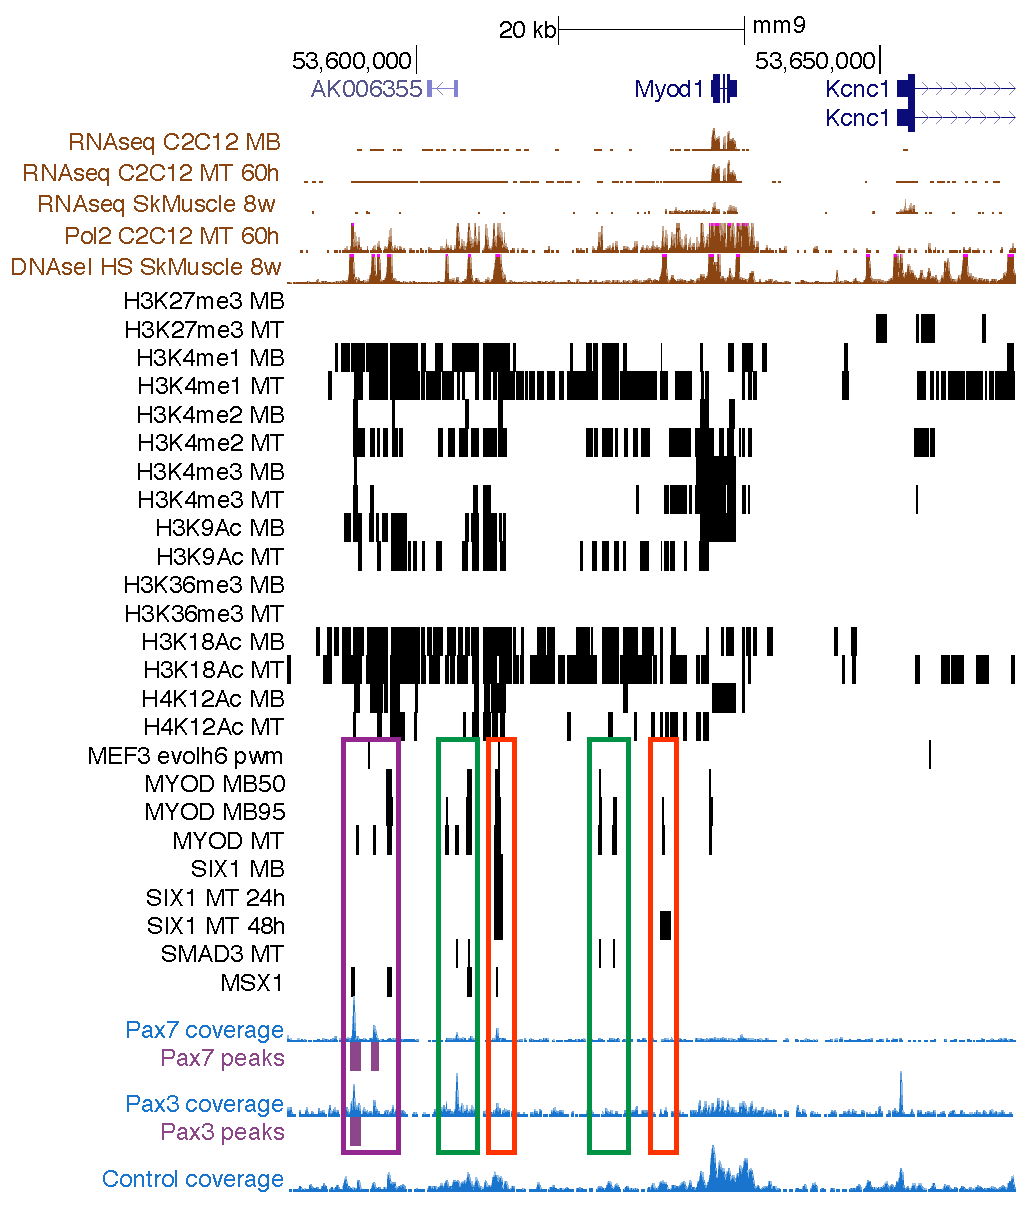
\includegraphics[width=1\textwidth]{figures/muscle/UCSC_myod1.pdf}
\captionbf{Visualisation de donn�es musculaires sur UCSC}{

    Capture d'�cran du navigateur de UCSC (UCSC Genome Browser,
    \url{http://genome.ucsc.edu}) montrant le locus de \textit{Myod1} et
    incluant un certain nombre des donn�es que nous avons recueillies.
    L'int�gration des donn�es permet de conduire rapidement plusieurs analyses
    sur la r�gulation g�n�tique (voir texte principal). Les cadres color�s
    indiquent des r�gions de r�gulation potentielles fix�es par MyoD (cadre
    pourpre avec Pax$3$ et Pax$7$, vert avec Smad3), ainsi que le \textit{Core
    Enhancer} CE (cadre rouge de gauche) et le \textit{Distal Regulatory
    Region} DRR (cadre rouge de droite). L'ensemble de ces enhancers constitue
    un \textit{super enhancer} (voir \ref{sub:les_super_enhancers} et
    \citet{Whyte2013tg}).

}
\label{fig:muscle/UCSC_myod1}
\efigp


Parmi ces donn�es figurent d'abord des exp�riences issues du projet ENCODE
(pr�sent� dans l'introduction en section \ref{sub:projet_encode}). Celles-ci
sont de plusieurs types et ont �t� obtenues par des laboratoires diff�rents. Il
y a notamment des donn�s RNAseq, quantifiant pr�cis�ment la transcription d'ARN
dans diff�rentes conditions (\cd � Caltech, muscle squelettique � University of
Washington ou UW), des donn�es d'hypersensibilit� � la digestion par DNAseI
(voir \ref{sub:chip_DNAseI}) en muscle adulte (UW) ainsi que diverses donn�es
de \chipseq de TFs en \cd (Caltech).  Parall�lement, nous avons obtenu
plusieurs donn�es � partir de la litt�rature. Par exemple, nous avons recueilli
les donn�es \chipseq de \citet{Asp2011p2370} pour $10$ marques �pig�n�tiques
sur les histones de cellules \cd cultiv�es en milieu de prolif�ration (MB pour
myoblastes) et en milieu de diff�renciation (MT pour myotubes). Nous avons
aussi recueilli des donn�es \chipseq pour divers TFs impliqu�s dans la
diff�renciation musculaire : le TF ma�tre MyoD en \cd MB et MT
\cite{Cao2010p1805}, les TFs Pax$3$ et Pax$7$ marquant respectivement les
prog�niteurs embryonnaires et les cellules satellites, ou prog�niteurs adultes,
obtenus dans des myoblastes primaires \cite{Soleimani2012p3753}, le TF Smad$3$
associ� � la voie TGF-$\beta$ en MT \cite{Mullen2011p3259}, le TF Msx$1$
permettant le recrutement du groupe Polycomb associ� aux marques r�pressives
H$3$K$27$me$3$ en \cd MB \cite{Wang2011p2929}, ou encore le TF Sox$6$ impliqu�
dans l'inhibition des g�nes sp�cifiques des fibres lentes lors de la
diff�renciation terminale en myoblastes primaires � E$18$ \cite{An2011p2926}.
Par ailleurs, certains TFs n'ont pour le moment �t� �tudi�s que par des
exp�riences de \chipchip � la r�solution et l'�tendue limit�e : le TF Gli
associ� � la voie de signalisation \textit{Sonic hedgehog} (SHH), dont les
donn�es ont �t� obtenues dans le bourgeon de membre d'embryons � E$11.5$
\cite{Vokes2008p1808}, ou encore le TF Six$1$ en \cd MB et MT
\cite{Liu2010p588}. Dans ce dernier cas, les donn�es ne couvrent que $17\%$ du
g�nome et poss�dent une faible r�solution ($\sim 1$kb) : elles sont donc
seulement compl�mentaires aux pr�dictions obtenues en utilisant la PWM MEF$3$
introduite pr�c�demment, car elles confirment la fixation de Six$1$ sur
certains des sites pr�dits (mais n'infirme pas l'absence de fixation des
prot�ines de la famille Six sur les autres sites).\\

Nous pr�sentons en figure \ref{fig:muscle/UCSC_myod1} un exemple montrant la
visualisation d'une partie des donn�es recueillies dans le cas du locus de
\textit{Myod$1$}, g�ne associ� aux prot�ines MyoD. Des informations sur la
position g�nomique et les transcrits pr�sents au sein du locus sont d'abord
donn�es dans la partie sup�rieure. Puis les pistes suivantes indiquent diverses
exp�riences, avec la nomenclature suivante : MB pour myoblaste (avec parfois le
pourcentage de confluence des cellules en culture), MT pour myotube (avec
parfois le temps pass� en milieu de diff�renciation), SkMuscle $8$w pour muscle
squelettique adulte � $8$ semaines post-natales et GM pour \textit{Growth
Medium}.  Les premi�res pistes de donn�es (en brun) sont issues du projet
ENCODE, les pistes suivantes (en noir) indiquent les coordonn�es des pics
\chipseq des marques �pig�n�tiques des histones ainsi que de divers TFs.  Les
pistes bleues pour Pax$3$ et Pax$7$ indiquent les donn�es brutes du nombre de
s�quences de \chipseq par nucl�otide, les segments pourpres indiquant les pics.
On montre aussi le contr�le de cette exp�rience (input) auquel les donn�es sont
compar�es pour d�finir les pics. Ainsi, le pic des donn�es brutes de Pax$3$
dans la partie droite de la piste n'est pas d�tect� comme un pic authentique
car les donn�es contr�le y poss�dent aussi un pic.

Prises ensemble, ces donn�es permettent d'appr�hender la r�gulation du g�ne
\textit{Myod$1$} au cours de la diff�renciation musculaire. D'abord,
\textit{Myod$1$} est transcrit au cours de la diff�renciation des cellules \cd
(d�tection d'ARN par RNAseq, traces de PolII marquant la transcription) mais
son expression est plus faible en muscle adulte, soit longtemps apr�s la
diff�renciation. Le g�ne est dans une r�gion de chromatine ouverte (DNAseI HS),
et c'est aussi le cas pour plusieurs r�gions alentour. Les pics de DNAseI HS
sont notamment corr�l�s aux pics de PolII ainsi qu'� d'autres TFs comme
MyoD\footnote{Il est effectivement connu que \textit{Myod1}
s'autor�gule~\cite{Thayer1989kx}}, Six$1$, Msx$1$, Pax$3$ ou encore Pax$7$, et
� des marques epig�n�tiques \og activatrices \fg comme les m�thylation
d'histone H$3$K$4$me$1$, H$3$K$4$me$2$ et H$3$K$4$me$3$ ou l'ac�tylation
H$3$K$9$Ac, qui sont toutes renforc�es au cours de la diff�renciation (passage
de MB � MT).  Le fait que l'on observe des pics de PolII hors des r�gions
transcrites est d� � l'interaction entre des r�gions de r�gulation contenant
plusieurs TFs et le promoteur du g�ne r�gul� (ici \textit{Myod1}) fixant la
polym�rase. Ces donn�es pointent donc vers l'existence de multiples r�gions de
r�gulation � la chromatine ouverte et interagissant avec le promoteur de
\textit{Myod$1$}. Plus pr�cis�ment, on trouve de gauche � droite : une r�gion
fixant Pax$3$, Pax$7$, Msx$1$ et MyoD en diff�renciation tardive qui pourrait
par exemple �tre impliqu�e dans la diff�renciation des cellules satellites
(cadre pourpre), plusieurs r�gions fixant Smad$3$ et MyoD pouvant peut-�tre
servir � int�grer des signaux TGF-$\beta$ (cadres verts), ainsi que deux
r�gions r�gulatrices connues (cadres rouges), l'une \cite{Kucharczuk1999zr}
fixant MyoD, Six$1$ et Msx$1$ tout au long de la diff�renciation et poss�dant
un site MEF$3$ conserv� (le CE de MyoD, impliqu� dans la diff�renciation des
prog�niteurs embryonnaires), et l'autre \cite{Asakura1995ly} fixant Six$1$ et
MyoD en MT (le DRR, impliqu� chez l'embryon ainsi que dans le muscle adulte).
Ces enhancers semblent donc avoir diff�rent r�les dans l'activation de
\textit{Myod$1$} et la mise en place de la myogen�se. On notera pour finir que
l'ensemble de ces r�gions de r�gulation, � forte densit� de \chipseq pour le TF
ma�tre MyoD et associ�es � des marques �pig�n�tiques extensives, a �t� d�fini
ailleurs comme un \textit{super-enhancer} (voir \ref{sub:les_super_enhancers}
et \citet{Whyte2013tg}).\\


L'int�gration des donn�es exp�rimentales et bioinformatiques li�es � la
r�gulation du ph�notype musculaire permet ainsi de visualiser rapidement la
r�gulation possible d'un g�ne et de proposer des hypoth�ses de m�canismes
sous-jacents, qu'il s'agit ensuite de valider exp�rimentalement. Nous avons pu
partager la session UCSC contenant ces diff�rentes donn�es avec nos
collaborateurs au sein de l'�quipe de P. Maire, qui ont maintenant la
possibilit� de croiser et interpr�ter rapidement un grand nombre de donn�es
publi�es ainsi que de donn�es obtenues au cours de cette th�se.

% subsection obtention_de_donn_es_partir_de_la_litt_rature_et_int_gration_ucsc (end)

\section{Pr�dictions et validations de la r�gulation par Six} 
\label{sec:pr_dictions_et_validations_de_la_r_gulation_par_six}

Plusieurs pr�dictions r�alis�es gr�ce � la PWM \mef ont �t� r�alis�es et
valid�es exp�rimentalement, nous en pr�sentons ici deux majeures.

\subsection{R�gulation de \textit{Myod1} par les prot�ines Six chez l'embryon de souris}
\label{sub:r_gulation_de_myod1_par_les_prot_ines_six}

\bfig
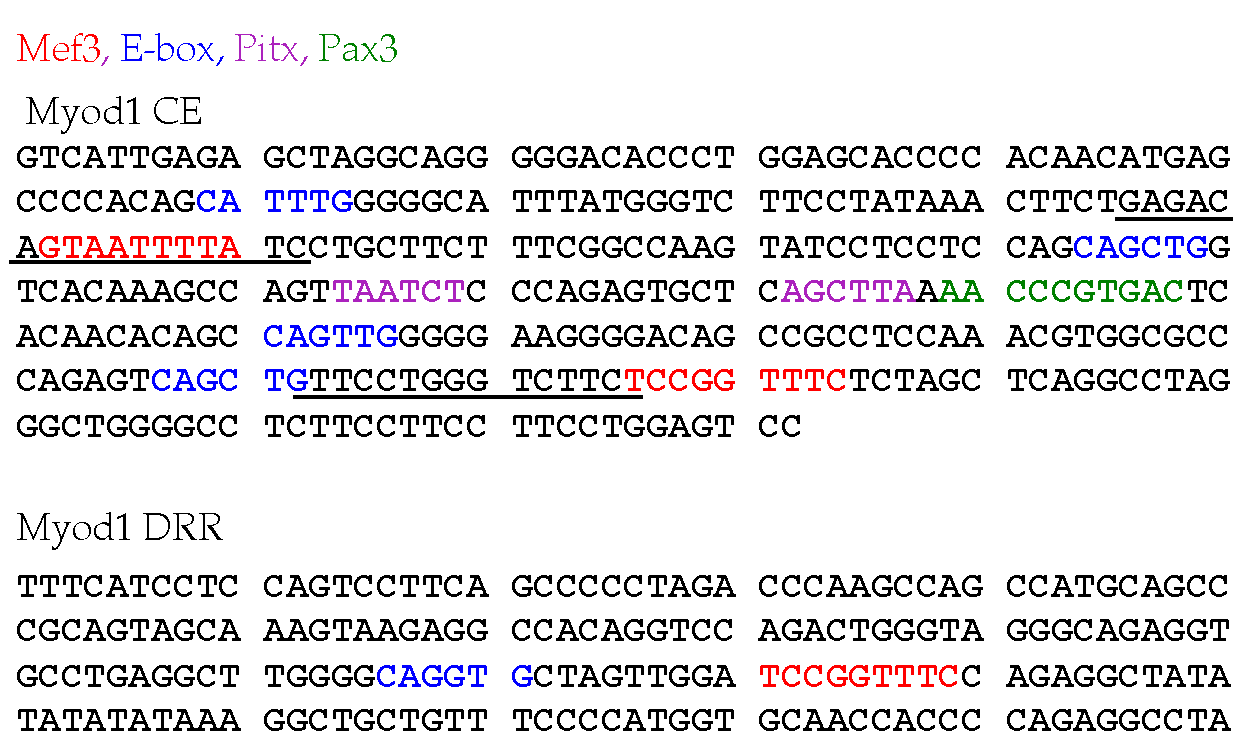
\includegraphics[width=1\textwidth]{figures/muscle/myod_ce_drr_sequences.pdf}
\captionbf{Pr�diction de sites \mef sur les s�quences r�gulatrices CE et DRR de \textit{Myod1}}{

    S�quences correspondant aux r�gions r�gulatrices CE et DRR de
    \textit{Myod1}.  Trois sites \mef ont �t� pr�dits � des scores respectifs
    de $7$ bits pour le premier du CE (CE$1$) et $11.1$ bits pour le deuxi�me
    du CE (CE$2$) et celui du DRR. Le seuil de $7$ bits correspond au seuil
    minimal trouv� en fig. \ref{fig:muscle/roc-mef3} comme discernant positifs
    de n�gatifs. Les sites E-Box, Pitx et Pax3 indiqu�s correspondent � des
    sites d�j� valid�s. Les s�quences soulign�es correspondent aux bo�tes LS$4$
    et LS$15$ de l'exp�rience de \textit{Linker-Scanner Mutagenesis} du CE
    humain r�alis�e par \citet{Kucharczuk1999zr} et sont requises pour
    l'expression dans les lign�es musculaires.

}
\label{fig:muscle/myod_ce_drr_sequences}
\efig

Nous avons d'abord r�alis� des pr�dictions de sites \mef sur deux enhancers
connus de \textit{Myod1}, le \textit{Core Enhancer} CE et le \textit{Distal
Regulatory Region} DRR, qui ont �t� publi�es dans l'article
\citet{Relaix2013ve} paru dans \textit{Plos Genetics}. Les pr�dictions ont �t�
r�alis�es avec un seuil de $7$ bits\footnote{Il faut noter que le seuil utilis�
    pour afficher les sites \mef conserv�s dans le navigateur de UCSC en figure
    \ref{fig:muscle/UCSC_myod1} est plus �lev� ($10.5$ bits). En effet,
    � l'�chelle g�nomique, il y a une tr�s grande quantit� de sites n�gatifs,
    et il faut donc aller vers les petits taux de Faux Positifs (ou les hauts
    seuils de d�tection) pour assurer un filtrage du bruit suffisant : par
    exemple, on trouve un site non conserv� tous les $2^7 \sim 128$ bp pour un
    seuil de $7$ bits, contre $2^{10.5} \sim 1500$ pour un seuil de $10.5$
    bits. En ajoutant le crit�re de conservation, ces quantit�s sont plus
petites, et le seuil de $7$ bits para�t raisonnable pour des pr�dictions sur
des s�quences de petite taille $\sim200$ bp.  } correspondant au seuil de
distinction optimal de sites \mef positifs et n�gatifs introduit en figure
\ref{fig:muscle/roc-mef3}.  Nous avons ainsi d�tect� $2$ sites \mef sur le CE
et $1$ sur le DRR que nous montrons en figure
\ref{fig:muscle/myod_ce_drr_sequences}. Sur le CE, les deux sites recoupent en
partie des �l�ments essentiels � l'expression \invivo du CE humain dans les
cellules musculaires myotomales de la souris \cite{Kucharczuk1999zr}. Nous
montrons par ailleurs d'autres sites d�tect�s dans des travaux pr�c�dents
\cite{Lhonore2010p3969,Kucharczuk1999zr}  : les sites Pitx$2$ et Pax$3$ dans le
CE, ou encore les E-box dans le CE et le DRR.\\


\bfigp
\includegraphics[width=1\textwidth]{figures/muscle/myod_ce_drr_mutations_relaix.pdf}
\captionbf{Validation des sites \mef pr�dits dans les �l�ments r�gulateurs de \textit{Myod1}}{

    Figure pr�sent�e dans l'article \citet{Relaix2013ve}. Plus de d�tails sont
    donn�s dans le texte principal. (A) Exp�rience de \chip montrant que les
    prot�ines Eya, cofacteurs de Six$1$ et Six$4$, sont recrut�es au niveau du
    CE et du DRR. (B) Exp�riences de retard sur gel (EMSA) montrant  que Six$1$
    et Six$4$ interagissent avec les sites pr�dits sur les enhancers.  (C)
    Sch�ma des transg�nes wild-type et mut�s en sites \mef. (D) Coloration au
    X-Gal d'embryons � E$12.5$ porteurs de transg�nes des s�quences wild-type
    (a, b, c) et mutantes (d, e, f), montrant l'abolition du g�ne rapporteur
    lorsque les sites \mef sont mut�s.  (E) Analyse de l'expression de MyoD par
    immunohistochimie et du rapporteur LacZ par coloration X-Gal dans les
    coupes indiqu�es par un trait noir chez les embryons c, d, e et f au niveau
    du thorax (Th) et des yeux (Eye). On note l'absence d'expression du
    transg�ne mut� dans les cellules exprimant MyoD.

}
\label{fig:muscle/myod_ce_drr_mutations_relaix}
\efigp

La validation de ces pr�dictions est pr�sent�e en figure
\ref{fig:muscle/myod_ce_drr_mutations_relaix}. Tout d'abord, il est montr� par
retard sur gel que les prot�ines Six$1$ et Six$4$ se fixent effectivement sur
les s�quences pr�dites (fig.~\ref{fig:muscle/myod_ce_drr_mutations_relaix}B).
Dans cette exp�rience, des oligonucl�otides marqu�s par la radioactivit�
contenant le site \mef consensus GAAACCTGA du promoteur de Myog sont incub�s
avec les prot�ines Six$1$ et Six$4$ synth�tis�es \invitro (colonne $1$). On
ajoute ensuite des oligonucl�otides non marqu�s en exc�s d'un facteur $60$ ou
$300$ et contenant le site \mef de Myog (contr�le positif, colonnes $2$ et
$3$), les sites \mef du DRR (colonnes $4$ et $5$) et du CE (site $1$ : colonnes
$6$ et $7$, site $2$ : colonnes $8$ et $9$), ou le site NFI  du promoteur de
Myog (contr�le n�gatif, colonne $10$, exc�s de $300$). Ensuite, il est montr�
que la mutation des sites \mef abolit l'expression d'un rapporteur \invivo de
l'activit� des enhancers par transgen�se. Pour cela, deux constructions ont �t�
r�alis�es, contenant le CE, le DRR ainsi que le promoteur PRR (\textit{Proximal
Regulatory Region}) de \textit{Myod1} en amont du g�ne rapporteur LacZ, avec ou
sans mutations au niveau des $3$ sites \mef pr�dits
(fig.~\ref{fig:muscle/myod_ce_drr_mutations_relaix}C). Ces constructions ont
�t� introduites dans des embryons par transgen�se transitoire, et ceux-ci sont
pr�lev�s � E$12.5$ puis l'expression de LacZ est r�v�l�e par coloration au
X-Gal (fig.~\ref{fig:muscle/myod_ce_drr_mutations_relaix}D). Au total, $6$
transg�nes \textit{wild-type} sur $10$ expriment le rapporteur
LacZ\footnote{Cette variation d'expression est notamment due au fait qu'il est
difficile de contr�ler le nombre de transg�nes ins�r�s dans le g�nome.} avec un
motif d'expression st�r�otyp� (les $3$ plus forts d'entre eux sont montr�s sur
la figure). Dans le cas des transg�nes mut�s, $3$ sur $8$ expriment tr�s
l�g�rement LacZ, ils sont tous montr�s sur la figure. Enfin, des sections
r�alis�es au niveau de la t�te et du thorax montre que l'expression du
rapporteur du transg�ne \textit{wild-type} r�capitule le motif d'expression du
g�ne \textit{Myod1} endog�ne, alors que pour les transg�nes mut�s l'expression
est tr�s rare : ainsi, MyoD seul ne peut activer le rapporteur \textit{via} les
E-Box.
  
  %Ainsi, le nombre de transg�nes ins�r�s dans les embryons positifs
  %(X-Gal+) varie entre $3$ et $34$, alors que pour les n�gatifs il varie entre
  %$1$ et $14$. 
%The number of transgenes inserted was 23 (f), 39
%(d) and 40 (e) for X-Gal+ embryos, and from 1 to 51 for X-Gal2 embryos. F-

% subsection r_gulation_de_myod1_par_les_prot_ines_six (end)

\subsection{R�gulation d'un lincRNA par Six dans le muscle adulte}
\label{sub:r_gulation_d_un_lincrna_par_six_dans_le_muscle_adulte}

Nous pr�sentons maintenant un travail r�alis� en collaboration avec Iori
Sakakibara de l'�quipe de P. Maire.

\subsubsection{Contexte g�n�ral}

\bfigp
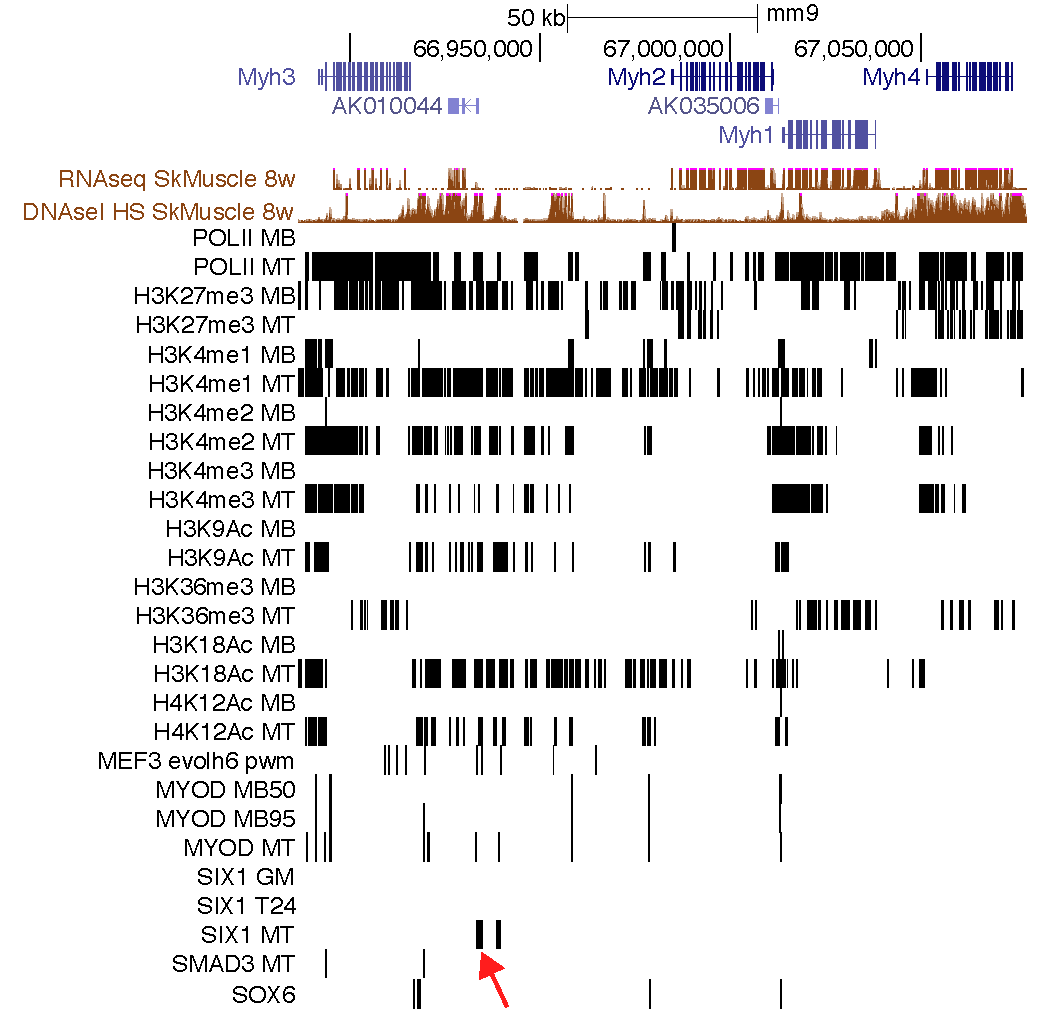
\includegraphics[width=1\textwidth]{figures/muscle/UCSC_lincMYH.pdf}
\captionbf{Visualisation du locus des myosines sur UCSC}{

    Le locus des myosines s'�tend sur $300$ kb sur le chromosome $11$ de la
    souris. Au sein de ce locus ce trouve un long ARN non codant (linc-RNA),
    AK$010044$ ou linc-MYH. Ce lincRNA est transcrit dans le muscle
    squelettique (RNAseq), o� il se trouve au sein d'un r�gion de chromatine
    ouverte (DNAseI HS). La r�gion est marqu�e par une forte r�gulation
    �pig�n�tique lors de la diff�renciation des \cd : apparition de marques
    d'activation (H$3$K$4$me et diverses ac�tylations) et disparition de marque
    inhibitrices (H$3$K$27$me$3$), ces changements �tant corr�l�s avec des
    traces �tendues sur le locus de PolII.  Linc-MYH est entour� de r�gions de
    r�gulation putatives contenant les TFs MyoD, Six$1$, Smad$3$ et Sox$6$.
    Ici, nous nous sommes concentr�s sur la r�gion directement en amont du TSS
    de lincMYH (indiqu�e par une fl�che rouge), contenant des traces \chipseq
    pour MyoD et Six$1$ en MT, ainsi que plusieurs sites MEF$3$ conserv�s
    � haut score.

}
\label{fig:muscle/UCSC_lincMYH}
\efigp

Les prot�ines Six poss�dent un r�le important dans la sp�cialisation des fibres
musculaires de type rapide (ou glycolytiques) lors de la diff�renciation
tardive~\cite{Niro2010p3444}. De plus, dans le muscle adulte, Six$1$ est
exprim� de mani�re plus importante dans les noyaux des fibres adultes que dans
ceux des fibres lentes. Le ph�notype rapide est marqu� par l'expression de
g�nes \og rapides \fg, dont les troponines \textit{Tnnt$3$}, \textit{Tnni$2$}
et \textit{Tnnc$2$} ou les myosines \textit{Myh$2$}, \textit{Myh$1$} et
\textit{Myh$4$}. La question concernant le r�le exact des prot�ines Six lors de
cette sp�cialisation est encore ouverte .\\

Nous avons concentr� notre �tude sur le \og cluster myosines \fg s'�tendant sur
$300$ kb dans le chromosome $11$ de la souris, et contenant les myosines
\textit{Myh$3$} (embryonnaire), \textit{Myh$2$} (rapide de type $2$A),
\textit{Myh$1$} (rapide de type $2$X), \textit{Myh$4$} (rapide de type $2$B),
\textit{Myh$8$} (p�rinatale) et \textit{Myh$13$} (extra-oculaire). Nous
montrons en fig.~\ref{fig:muscle/UCSC_lincMYH} une partie de ce locus. Nous
nous sommes demand�s si les prot�ines Six pouvaient r�guler directement les
myosines de type rapide au niveau de ce locus. La concentration des g�nes de
myosine en un m�me locus est r�miniscente du cluster des g�nes de la
$\beta$-globine. Dans ce cluster, les diff�rents g�nes de la $\beta$-globine
sont r�gul�s par une m�me r�gion r�gulatrice, appel�e \og Locus Control Region
\fg ou LCR~\cite{Palstra2008dq}. Nous avons donc cherch� � savoir si un tel LCR
pouvait exister dans le cas du cluster myosine.\\

Nous avons ainsi centr� notre attention sur une r�gion de chromatine ouverte
fix�e par Six$1$ et MyoD en cellules \cd et contenant plusieurs sites \mef
(indiqu�e par une fl�che rouge dans la figure \ref{fig:muscle/UCSC_lincMYH}).
Cette r�gion est situ�e � proximit� des myosines de type rapide, et se trouve
en amont du TSS d'un long ARN non codant ou lincRNA (pour \textit{long
intergenic non-coding RNA}) que nous avons nomm� linc-MYH.  Les linc-RNAs ont
re�u beaucoup d'attention ces derni�res ann�es du fait des r�les vari�s qu'on
leur a d�couverts, notamment au niveau de la r�gulation de la
chromatine~\cite{Rinn2012cr}. Nous nous sommes donc pos�s deux questions
: est-ce que cette r�gion de r�gulation peut servir de LCR aux myosines de type
rapide? Et peut-elle servir � activer linc-MYH, qui pourrait alors avoir un
r�le dans le processus de sp�cialisation?

\subsubsection{Article}

Dans l'article qui suit, il est d'abord montr� que cette r�gion r�gulatrice
fix�e par Six$1$ sert de LCR aux myosines rapides. Ainsi, elle interagit
\invivo avec les promoteurs des myosines rapides. Elle active par ailleurs des
g�nes rapporteurs sous le contr�le des promoteurs de \textit{Myh$2$},
\textit{Myh$1$}, \textit{Myh$4$}, et cette activit� est abolie lors de la
mutation des sites \mef. Par ailleurs, il est montr� que ce LCR est capable
d'activer linc-MYH. Le r�le de linc-MYH est �tudi� par KO dans un muscle adulte
de type rapide par �lectroporation d'un shRNA. Ce KO r�sulte en une
augmentation significative de l'expression des g�nes associ�s au ph�notype
lent, comme \textit{Tnnt$1$}, \textit{Tnni$1$} et \textit{Tnnc$1$}. Ainsi, en
se fixant sur le LCR, Six$1$ jour un double r�le : localement, il permet
l'activation les myosines de type rapide, et � l'�chelle du g�nome, il bloque
le programme d'expression de g�nes lents \textit{via} l'activation de linc-MYH,
permettant \textit{in fine} la mise en place du programme rapide.

\newpage

%\includepdf[pages=-]{articles/muscle-lincMYH/manuscript.pdf}
%%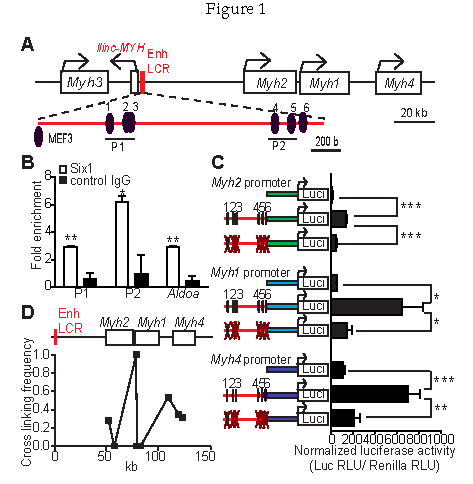
\includepdf[pages=-]{articles/muscle-lincMYH/Sakakibara_figure_1.pdf}
%%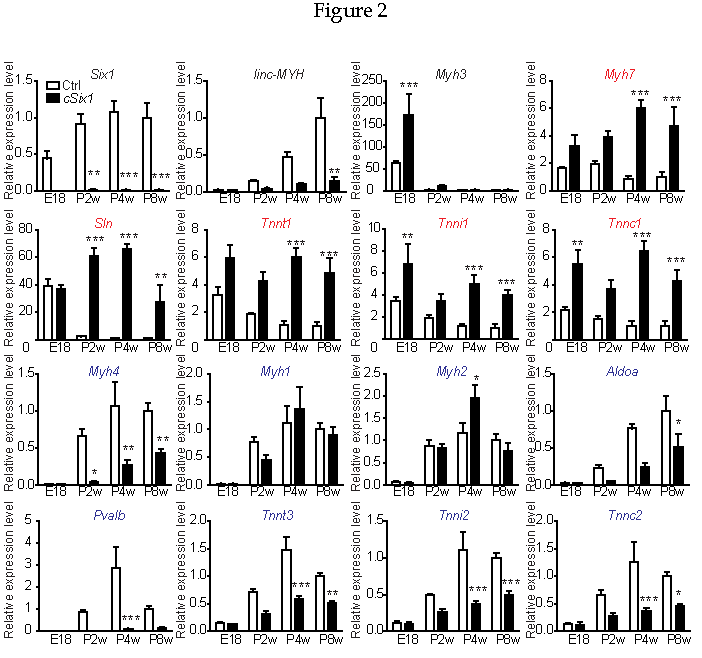
\includepdf[pages=-]{articles/muscle-lincMYH/Sakakibara_figure_2.pdf}
%%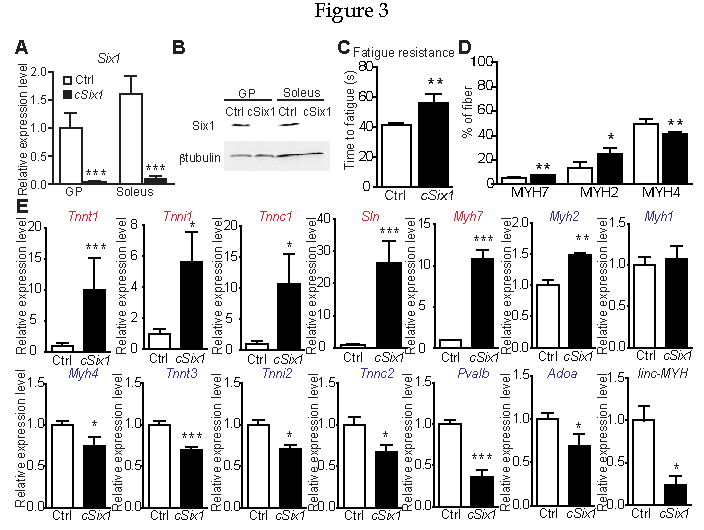
\includepdf[pages=-]{articles/muscle-lincMYH/Sakakibara_figure_3.pdf}
%%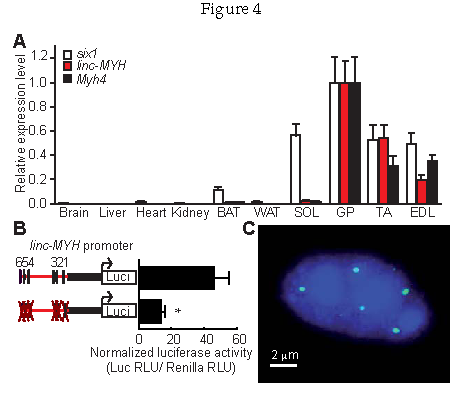
\includepdf[pages=-]{articles/muscle-lincMYH/Sakakibara_figure_4.pdf}
%%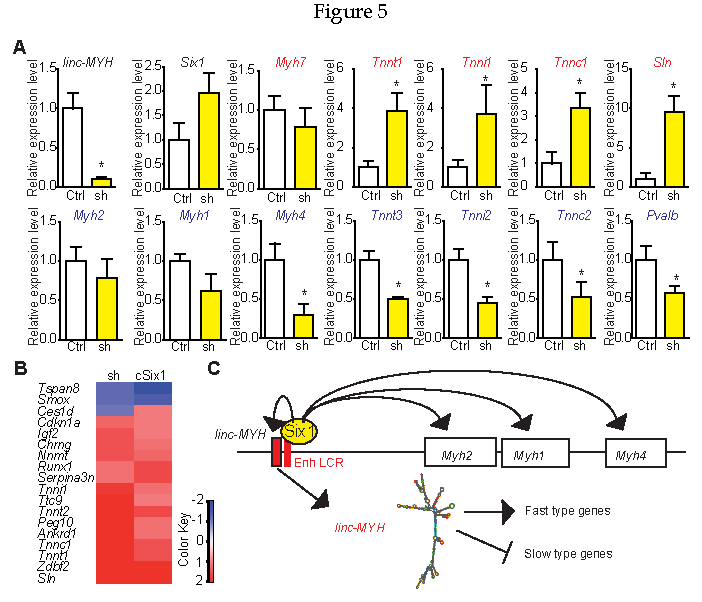
\includepdf[pages=-]{articles/muscle-lincMYH/Sakakibara_figure_5.pdf}
%%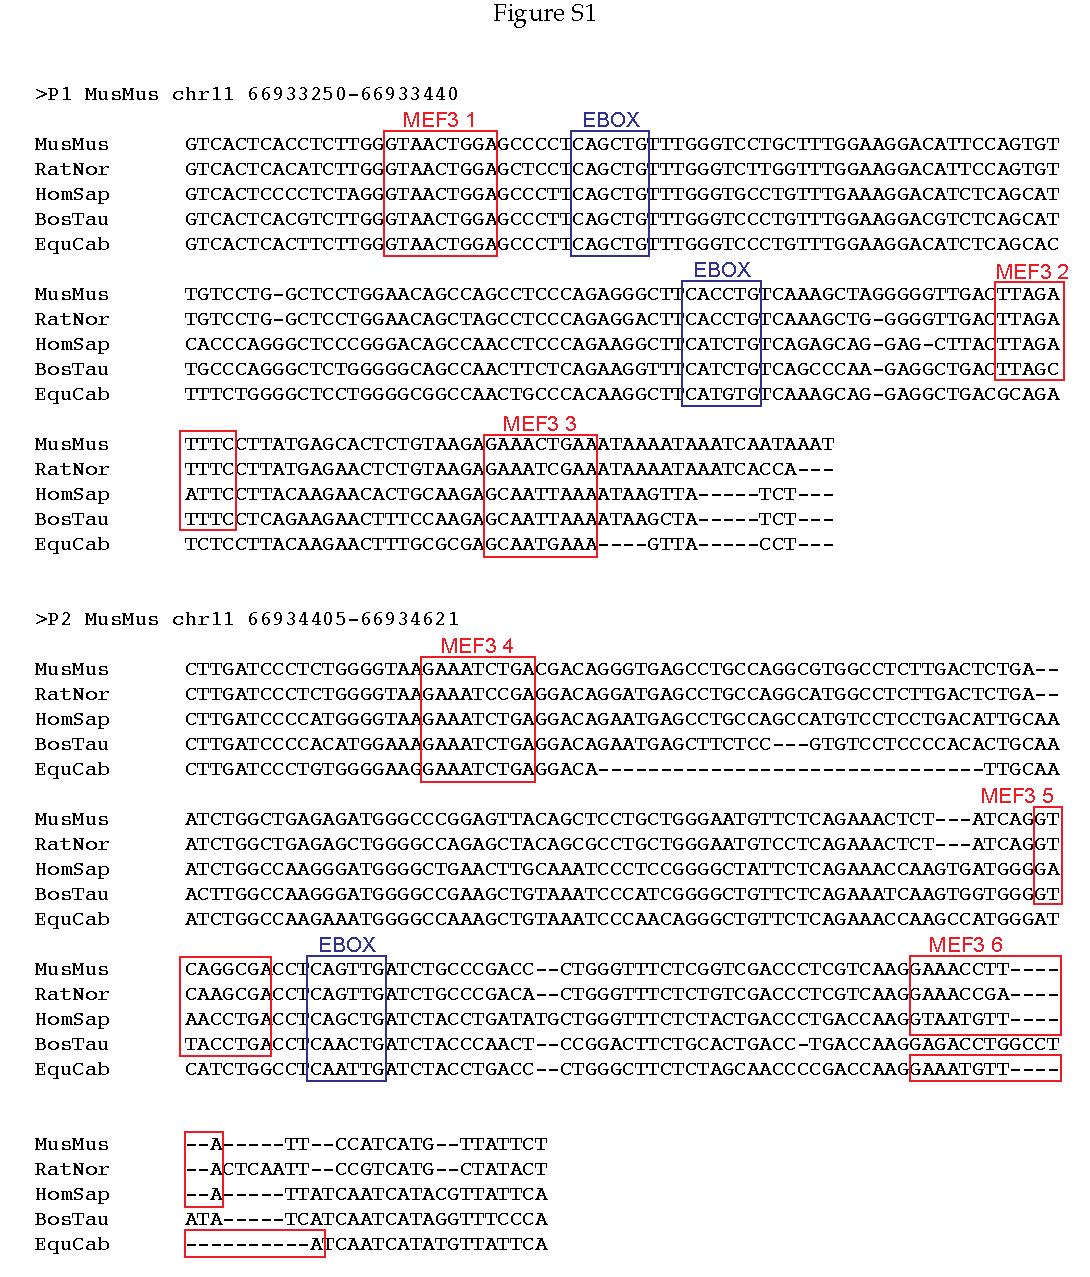
\includepdf[pages=-]{articles/muscle-lincMYH/Sakakibara_supplemental_figure_1.pdf}
%%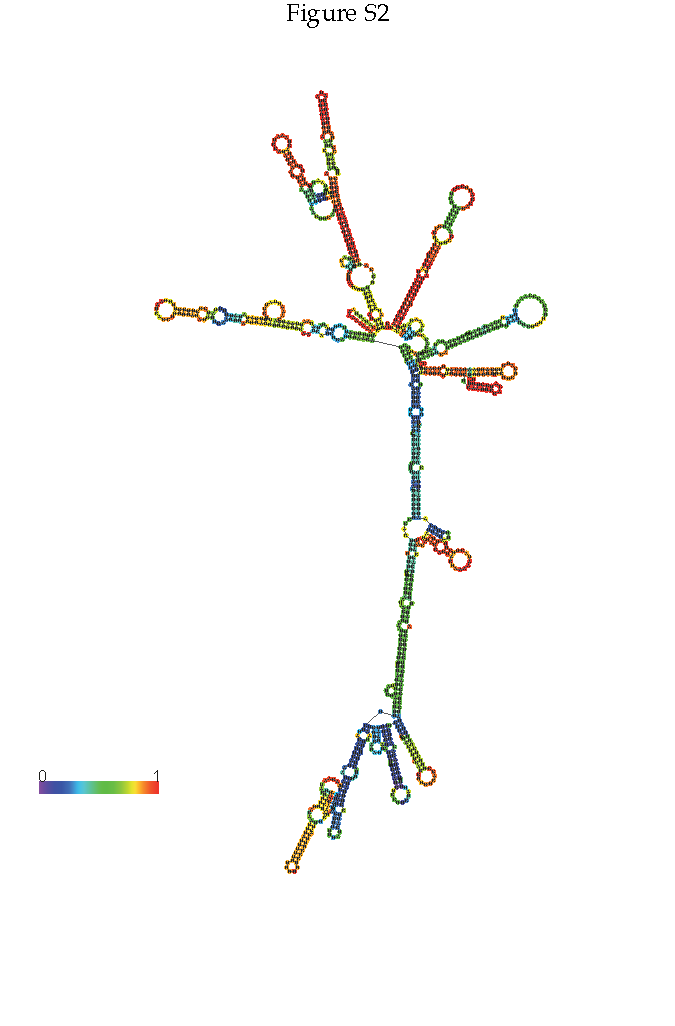
\includepdf[pages=-]{articles/muscle-lincMYH/Sakakibara_supplemental_figure_2.pdf}
%%\includepdf[pages=-]{articles/muscle-lincMYH/Sakakibara_supplemental_figure_3.pdf}
%%\includepdf[pages=-]{articles/muscle-lincMYH/Sakakibara_supplemental_figure_4.pdf}
%%\includepdf[pages=-]{articles/muscle-lincMYH/Sakakibara_supplemental_figure_5.pdf}
%%\includepdf[pages=-]{articles/muscle-lincMYH/Table_S3.pdf}
%%\includepdf[pages=-]{articles/muscle-lincMYH/Table_S4.pdf}

% subsection r_gulation_d_un_lincrna_par_six_dans_le_muscle_adulte (end)


% section pr_dictions_et_validations_de_la_r_gulation_par_six (end)
			


%%%%%%%%%%%%%%%%%%%%%%%%%%%%%%%%%%%%%%%%%%%%%%%%%%%%%%%%%%%%%%%%%%%%%%%%%%%%%%%%%%%%%%%%%%%%%%%%%%%	%%%%%%%%%%%%%%%%%%%%%%%%%%%%%%%%%%%%%%%%%%%%%%%%%%%%%%%%%%%%%%%%%%%%%%%%%%%%%%%%%%%%%%%%%%%%%%%%%%%	
\newpage	
			
\section*{Conclusion du chapitre \thechapter}

%\newpage

%%%%%%%%%%%%%%%%%%%%%%%%%%%%%%%%%%%%%%%%%%%%%%%%%%%%%%%%%%%%%%%%%%%%%%%%%%%%%%%%%%%%%%%%%%
%\chapter{\ChTest}\ifthenelse{\FaitMinitocs > 0}{\minitoc}{Minitoc}
%\newpage
%\input{chapters/Chapter-test}
%\newpage
%%%%%%%%%%%%%%%%%%%%%%%%%%%%%%%%%%%%%%%%%%%%%%%%%%%%%%%%%%%%%%%%%%%%%%%%%%%%%%%%%%%%%%%%%%

%\newpage
\WriteThisInToc\addstarredchapter{Conclusion}\chapter*{Conclusion}\markboth{\slshape Conclusion\hfil}{\slshape Conclusion\hfil}


\vskip7mm

\noindent\textbf{\LARGE\sffamily\scshape R�sum�}

\medskip


\bs~\medskip

\noindent\textbf{\LARGE\sffamily\scshape Perspectives}

\medskip


%%%%%%%%%%%%%%%%%%%%%%%%%%%%%%%%%%%%%%%%%%%%%%%%%%%%%%%%%%%%%%%%%%%%%%%%%%%%%%%%%%%%%%%
%%%%%%%%%%%%%%%%%%%%%%%%%%%%%%%%%%%%%%%%%%%%%%%%%%%%%%%%%%%%%%%%%%%%%%%%%%%%%%%%%%%%%%%%%%
%\ifthenelse{\IncludeAnnexes > 0}{ 
%
\Annexes
\addtocontents{lof}{\protect\addvspace{10pt}}
\renewcommand{\thechapter}{A}
\setcounter{figure}{0}
\renewcommand{\leftmark}{Annexes}
\renewcommand{\rightmark}{Annexes}
 %\hrule
  \vspace{15pt}%
  {\Huge \fontfamily{ppl}\selectfont \textbf{Liste des Annexes}}
   \par\nobreak
    \vspace{15pt}
       \hrule
   \vskip20pt
	\normalsize

\begin{tabular}{lp{11.5cm}r}
	Annexe A & \hyperref[annexe-tableoptique]{Titre annexe}  \dotfill& \textbf{\pageref{annexe-tableoptique}}\\
	Annexe B & \hyperref[annex-freqpm]{Titre annexe}  \dotfill& \textbf{\pageref{annex-freqpm}}\\
	Annexe C & \hyperref[annexe-PRL]{Titre annexe}  \dotfill& \textbf{\pageref{annexe-PRL}}\\
	Annexe D & \hyperref[annexe-EPL]{Titre annexe}  \dotfill& \textbf{\pageref{annexe-EPL}}\\
	Annexe E & \hyperref[annexe-seqexptot]{Titre annexe} \dotfill& \textbf{\pageref{annexe-seqexptot}}\\
\end{tabular}

  \EmptyNewPage


%%%%%%%%%%%%%%%%%%%%%%%%%%%%%%%%%%%%%%%%%%%%%%%%%%%%%%%%%%%%%%%%%%%%%%%%%%%%%%%%%%%%%%%%%%%%%%%%%%	
%%%%%%%%%%%%%%%%%%%%%%%%%%%%%%%%%%%%%%%%%%%%%%%%%%%%%%%%%%%%%%%%%%%%%%%%%%%%%%%%%%%%%%%%%%%%%%%%%%	
\AnnexTitreCed{A}{Titre annexe}{annexe-tableoptique}
{
}

%%%%%%%%%%%%%%%%%%%%%%%%%%%%%%%%%%%%%%%%%%%%%%%%%%%%%%%%%%%%%%%%%%%%%%%%%%%%%%%%%%%%%%%%%%%%%%%%%%	
\AnnexTitreCed{B}{Titre annexe}{annex-freqpm}
{
}			 			 


%%%%%%%%%%%%%%%%%%%%%%%%%%%%%%%%%%%%%%%%%%%%%%%%%%%%%%%%%%%%%%%%%%%%%%%%%%%%%%%%%%%%%%%%%%%%%%%%%%	
\AnnexTitreCed{C}{Titre annexe}{annexe-PRL}
{
}

%%%%%%%%%%%%%%%%%%%%%%%%%%%%%%%%%%%%%%%%%%%%%%%%%%%%%%%%%%%%%%%%%%%%%%%%%%%%%%%%%%%%%%%%%%%%%%%%%%	
\AnnexTitreCed{D}{Titre annexe}{annexe-EPL}
{

%\includepdf[pages=-]{annexes/epl}  %% pour inclure un article directement en pdf!
}

%%%%%%%%%%%%%%%%%%%%%%%%%%%%%%%%%%%%%%%%%%%%%%%%%%%%%%%%%%%%%%%%%%%%%%%%%%%%%%%%%%%%%%%%%%%%%%%%%%	
\AnnexTitreCed{E}{Titre annexe}{annexe-seqexptot}
{

} 
%\Annexes
%\Annex{Statistiques g�nomique}
\begin{appendices}
\chapter{Statistiques g�nomique}
\label{ann:statistiques}

\begin{figure}
    \centering
    \includegraphics[width=1.0\textwidth]{figures/intergenic-intronic.pdf}
    \captionbf{Distribution des tailles interg�niques et introniques chez diff�rentes esp�ces}{

        
        Distributions log-log de la taille des r�gions interg�niques (A) et
        introniques (B) chez diff�rentes esp�ces. Les histogrammes sont
        r�alis�s avec un intervalle de $0.05$ puis liss�s avec l'estimateur local
        LOESS de param�tre $span = 0.3$ (logiciel R).
        (A)  Les r�gions interg�niques sont d�finies comme les
        r�gions compl�mentaires aux r�gions transcrites (donn�es UCSC),
        celles-ci �tant pr�alablement fusionn�es pour �viter les redondances
        li�es aux multiples transcrits d'un m�me g�ne. De la bact�rie
        � l'homme, on observe une inflation de la quantit� de g�nome non
        codant.  
        (B) Les r�gions introniques sont d�finies par le fait qu'elles sont
        entour�es par deux exons d'un m�me g�ne. Pour pouvoir �tre �piss�s lors
        de la maturation des preARNm, les introns doivent poss�der des sites
        d'�pissage, imposant une borne inf�rieure � leur taille pour que l'ARNm
        final soit fonctionnel.

    }
    \label{fig:intergenic-intronic}
\end{figure}

En guise d'exemple, nous montrons en figure \ref{fig:intergenic-intronic} des
statistiques obtenues ais�ment � partir d'annotations g�n�tiques pr�sentes sur
UCSC et trait�es avec Galaxy. Ces statistiques sont les distribution de tailles
des r�gions interg�niques et introniques chez plusieurs esp�ces : la bact�rie
\ecoli, la levure \textit{Saccharomyces cerevisiae}, le ver \celegans, la
mouche \dmel, la souris, le poulet et l'homme.
 
\end{appendices}
%}{}
%%%%%%%%%%%%%%%%%%%%%%%%%%%%%%%%%%%%%%%%%%%%%%%%%%%%%%%%%%%%%%%%%%%%%%%%%%%%%%%%%%%%%%%%%%%%%%

\EmptyNewPage 
\appendix 
\renewcommand{\leftmark}{Bibliographie}
\renewcommand{\rightmark}{Bibliographie} 
\bibliographystyle{custom}%biblio/paolostyle}
\BeginBibWith{\vskip7mm\noindent 
   Dans la version pdf, les num�ros de page sont
   des liens qui renvoient � l'occurence de la citation dans le texte.
}
\addcontentsline{toc}{chapter}{\bibname}
\bibliography{biblio/papers}

%%%%%%%%%%%%%%%%%%%%%%%%%%%%%%%%%%%%%%%%%%%%%%%%%%%%%%%%%%%%%%%%%%%%%%%%%%%%%%%%%%%%%%%%%%%%%%
%%%%%%%%%%%%%%%%%%%%%%%%%%%%%%%%%%%%%%%%%%%%%%%%%%%%%%%%%%%%%%%%%%%%%%%%%%%%%%%%%%%%%%%%%%%%%%
%\begin{ThesisAbstract}

	\begin{FrenchAbstract}
	
			Le r�sum� FR

	
			\KeyWords{Atomes froids, condensat de Bose-Einstein, puce � atomes, supraconductivit�, interactions atomes-surfaces.}
	\end{FrenchAbstract}
	
	\begin{EnglishAbstract}
	
		Le r�sum� EN
	
			\KeyWords{Cold atoms, Bose-Einstein condensate, atom chip, superconductivity, atom-surface interactions.}
	\end{EnglishAbstract}
	
\end{ThesisAbstract}

%%%%%%%%%%%%%%%%%%%%%%%%%%%%%%%%%%%%%%%%%%%%%%%%%%%%%%%%%%%%%%%%%%%%%%%%%%%%%%%%%%%%%%%%%%%%%%
%%%%%%%%%%%%%%%%%%%%%%%%%%%%%%%%%%%%%%%%%%%%%%%%%%%%%%%%%%%%%%%%%%%%%%%%%%%%%%%%%%%%%%%%%%%%%%
\end{document}
